% ****************************************************************************************** %
% Princeton University PhD Thesis template with CMake build system.
% The details are as follows:
%   Dissertation template and document class for Princeton University
%   Author  : Jeffrey Scott Dwoskin <jdwoskin@princeton.edu>
%   Adapted from:
%   http://www.math.princeton.edu/graduate/tex/puthesis.html
%   In git: https://github.com/zbeekman/PU-thesis-template
%   Minor edits and CMake based build system by:
%   Izaak Beekman
% Compilation of the LaTeX files is handled by CMake (CMake.org) and
% UseLATEX (https://github.com/kmorel/UseLATEX)
% ****************************************************************************************** %


%%% For print copies
%% set 'singlespace' option to set entire thesis to single space, and
%% define "\printmode" to remove all hyperlinks for printed copies of
%% the thesis. Delete all output files before changing this mode -- it
%% will turn hyperref package on and off

% CMake will turn this on if needed. This will override the digital
% and proquest options if they are set.

% @PRINTMODE_CTRL@\providecommand{\chooselayout}{\documentclass[@PUTHESIS_FONT_SIZE@@DRAFT@@LOT@@LOF@,singlespace]{puthesis}}
% @PRINTMODE_CTRL@\providecommand{\modifyoutput}{\newcommand{\printmode}{}}
% @PRINTMODE_CTRL@\providecommand{\fixupmargins}{\usepackage[hmarginratio=2:1]{geometry}}

% @DIGITALMODE_CTRL@\providecommand{\chooselayout}{\documentclass[@PUTHESIS_FONT_SIZE@@DRAFT@@LOT@@LOF@,twoside]{puthesis}}
% @DIGITALMODE_CTRL@\providecommand{\modifyoutput}{}
% @DIGITALMODE_CTRL@\providecommand{\fixupmargins}{\usepackage[hmarginratio=1:1]{geometry}}

%%% For the electronic copy, use double spacing
%%%%%%%%%%%%%%%%%%%%%
%%%%%  DEFAULT  %%%%%
%%%%%%%%%%%%%%%%%%%%%
\providecommand{\chooselayout}{\documentclass[12pt, lot,lof%,twoside
]{lib/puthesis}}
\PassOptionsToPackage{final}{hyperref}
\setlength{\marginparwidth}{2cm}
\providecommand{\modifyoutput}{}
\providecommand{\fixupmargins}{\usepackage[hmarginratio=2:1]{geometry}}

\chooselayout % Whatever is provided first as the definition will be
              % used
\modifyoutput


% define "\proquestmode"  to use outlined links, instead of colored
% links.

% Cmake will control this

% @PROQUESTMODE_CTRL@ \newcommand{\proquestmode}{}

% @DRAFTMODE_CTRL@ \providecommand{\maybefrontmatter}{}
\providecommand{\maybefrontmatter}{\makefrontmatter}

\fixupmargins

\setlength{\topmargin}{-.5in}
\setlength{\footskip}{.25in}
\setlength{\textheight}{9in}
\setlength{\textwidth}{6in}

% I prefer proquestmode to be off for electronic copies for normal use, since the colored links are less distracting. However when printed in black and white, the colored links are difficult to read.

%%% For early drafts without some of the frontmatter
% Also see the "ifodd" command below to disable more frontmatter
%\documentclass[12pt]{puthesis}

%%%%%%%%%%%%%%%%%%%%%%%%%%%%%%%%%%%%%%%%%%%%%%%%%%%%%%%%%%%%%\
%%%% Author & title page info

\title{ Concurrent Permission Machine for modular proofs of optimizing compilers 
with shared memory concurrency. }

\submitted{subm. Date}  % degree conferral date (January, April, June, September, or November)
\copyrightyear{tbd copyright}  % year in which the copyright is secured by publication of the dissertation.
\author{Santiago Cuellar}
\adviser{Andrew Appel}  %replace with the full name of your adviser
%\departmentprefix{Program in}  % defaults to "Department of", but programs need to change this.
\department{Computer Science}

%%%%%%%%%%%%%%%%%%%%%%%%%%%%%%%%%%%%%%%%%%%%%%%%%%%%%%%%%%%%%\
%%%% Tweak float placements
% From: http://mintaka.sdsu.edu/GF/bibliog/latex/floats.html "Controlling LaTeX Floats"
% and based on: http://www.tex.ac.uk/cgi-bin/texfaq2html?label=floats
% LaTeX defaults listed at: http://people.cs.uu.nl/piet/floats/node1.html

% Alter some LaTeX defaults for better treatment of figures:
    % See p.105 of "TeX Unbound" for suggested values.
    % See pp. 199-200 of Lamport's "LaTeX" book for details.
    %   General parameters, for ALL pages:
    \renewcommand{\topfraction}{0.85}	% max fraction of floats at top
    \renewcommand{\bottomfraction}{0.6}	% max fraction of floats at bottom
    %   Parameters for TEXT pages (not float pages):
    \setcounter{topnumber}{2}
    \setcounter{bottomnumber}{2}
    \setcounter{totalnumber}{4}     % 2 may work better
    \setcounter{dbltopnumber}{2}    % for 2-column pages
    \renewcommand{\dbltopfraction}{0.66}	% fit big float above 2-col. text
    \renewcommand{\textfraction}{0.15}	% allow minimal text w. figs
    %   Parameters for FLOAT pages (not text pages):
    \renewcommand{\floatpagefraction}{0.66}	% require fuller float pages
	% N.B.: floatpagefraction MUST be less than topfraction !!
    \renewcommand{\dblfloatpagefraction}{0.66}	% require fuller float pages

% The documentclass already sets parameters to make a high penalty for widows and orphans.

%%%%%%%%%%%%%%%%%%%%%%%%%%%%%%%%%%%%%%%%%%%%%%%%%%%%%%%%%%%%%\
%%%% Use packages

%\usepackage{amsfonts}

%%% For figures
\usepackage{graphicx}
%\usepackage{subfig,rotate}
%Verticall align tabular
\usepackage{array}

%Nicer footnotes
\usepackage{cprotect} %replace \footnote with \cprotect\footnote
%\usepackage{bigfoot}

%%% for comments
\usepackage{verbatim}


%%% For tables
\usepackage{multirow}
% Longtable lets you have tables that span multiple pages.
\usepackage{longtable}
%multicol allows multiple columns (we use this in tables)
\usepackage{multicol}

%For aligning enumerations and labels
\usepackage{calc}
\usepackage[shortlabels]{enumitem}  

% Booktabs produces far nicer tables than the standard LaTeX tables.
%   see: http://en.wikibooks.org/wiki/LaTeX/Tables
\usepackage{booktabs}

%Code highlight + specific highlights for coq
%\usepackage{minted}
\usepackage{listings}
\usepackage{xcolor}
\usepackage{lib/lstlangcoq}
% Several coq and C language settings


\lstdefinestyle{DecorateC}
{
language=C,
frame=tb,
mathescape=true,columns=fullflexible,
basicstyle=\ttfamily\footnotesize,
keywordstyle=\ttfamily\footnotesize\bfseries
}
\lstdefinestyle{C-inline}
{
language=C,
mathescape=true,columns=fullflexible,
basicstyle=\ttfamily,
keywordstyle=\ttfamily
}
\lstdefinestyle{C-inline-footnote}
{
language=C,
mathescape=true,columns=fullflexible,
basicstyle=\ttfamily\scriptsize,
keywordstyle=\ttfamily\scriptsize
}
\lstdefinestyle{C-list}
{
language=C,
mathescape=true,columns=fullflexible,
basicstyle=\ttfamily\small,
keywordstyle=\ttfamily\small\bfseries
}
\lstdefinestyle{Ltac-inline}
{
language=Coq,
mathescape=true,columns=fullflexible,
basicstyle=\sffamily,
keywordstyle=\sffamily
}
\lstdefinestyle{CoqGoal-list}
{
language=Coq,
mathescape=true,columns=fullflexible,
basicstyle=\sffamily,
keywordstyle=\sffamily\bfseries
}
\lstdefinestyle{CoqTheorem-inline}
{
language=Coq,
mathescape=true,columns=fullflexible,
basicstyle=\sffamily,
keywordstyle=\sffamily
}
\lstdefinestyle{CoqTheorem-list}
{
language=Coq,
mathescape=true,columns=fullflexible,
basicstyle=\sffamily,
keywordstyle=\sffamily\bfseries
}
\lstdefinestyle{CoqFootnote}
{
language=Coq,
mathescape=true,columns=fullflexible,
basicstyle=\sffamily\scriptsize,
keywordstyle=\sffamily\scriptsize
}


%%% Shortcuts for common language commands

%Inlined C code
\newcommand{\Ccode}[1]{\lstinline[language=C]{#1}}
\newcommand{\Coqcode}[1]{\lstinline[style=CoqTheorem-inline]{#1}}

% Set coq as default
\lstset{language=Coq,basicstyle=\sffamily,mathescape=true,columns=fullflexible}

%To draw stackframes.
\usepackage{lib/drawstack}


%set parameters for longtable:
% default caption width is 4in for longtable, but wider for normal tables
\setlength{\LTcapwidth}{\textwidth}


%Math letters like |P
\usepackage{ dsfont }
\usepackage{amsfonts} 
%Math stuff
\usepackage{amsmath}
\usepackage{amsthm}
\usepackage{aliascnt}
%for semantics [| and |]
\usepackage{stmaryrd}
% To add nice arrows for diagrams
\usepackage{tikz-cd}
% arranging formulas:
\usepackage{mathpartir} 
\usepackage{semantic}
%To make inference rules
\usepackage{lib/infrule}

%Has to go after amsmath
\ifdefined\boxdotright
\else
\usepackage{newtxmath} % Need this on Santiago's computer to get \boxdotright
\fi

%%For TODO's (HAS TO GO AFTER HYPERREF to get links working on drafts)
\usepackage[obeyDraft]{todonotes}
\usepackage{ifdraft}

%%%%%%%%%%%%%%%%%%%%%%%%%%%%%%%%%%%%%%%%%%%%%%%%%%%%%%%%%%
%%% Printed vs. online formatting
\ifdefined\printmode

% Printed copy
% url package understands urls (with proper line-breaks) without hyperlinking them
\usepackage{url}


\else

\ifdefined\proquestmode
%ProQuest copy -- http://www.princeton.edu/~mudd/thesis/Submissionguide.pdf

% ProQuest requires a double spaced version (set previously). They will take an electronic copy, so we want links in the pdf, but also copies may be printed or made into microfilm in black and white, so we want outlined links instead of colored links.
\usepackage[draft=false,final]{hyperref}
\hypersetup{final}
\PassOptionsToPackage{final}{hyperref}
\hypersetup{bookmarksnumbered}



% copy the already-set title and author to use in the pdf properties
\makeatletter
\hypersetup{pdftitle=\@title,
        pdfauthor=\@author}
\makeatother

\else
% Online copy

% adds internal linked references, pdf bookmarks, etc

% turn all references and citations into hyperlinks:
%  -- not for printed copies
% -- automatically includes url package
% options:
%   colorlinks makes links by coloring the text instead of putting a rectangle around the text.
\usepackage{hyperref}
\hypersetup{colorlinks,bookmarksnumbered}

% copy the already-set title and author to use in the pdf properties
\makeatletter
\hypersetup{pdftitle=\@title,
        pdfauthor=\@author}
\makeatother

% make the page number rather than the text be the link for ToC entries
%\hypersetup{linktocpage}
\fi % proquest or online formatting
\fi % printed or online formatting


%Clever references, better than autoref, prints lemma instead of theorem (even thout they share counter)
%HAS TO BE LOADED AFTER HYPERREF
\usepackage[nameinlink]{cleveref} 
\usepackage[shortlabels]{enumitem}


%Personal and group macros:

%%%%%%%%%%%%%%%%%%%%%%%%%%%%%%%%%%%%%%%%%%%%%%%%%%%%%%%%%%%%%%%%%%%%%%%
%% Rustan wants the letters in his math formulas to be spaced
%% as in running italic text.  So we here redefine each letter,
%% in its role as a MathSymbol, to come from the symbol font
%% named "italics", rather than from the one named "letters".

% The following line is needed to make this file work with certain
% fonts, include the standard Computer Modern fonts.
\DeclareSymbolFont{italics}{OT1}{cmr}{m}{it}

\DeclareMathSymbol{a}{\mathalpha}{italics}{"61}
\DeclareMathSymbol{b}{\mathalpha}{italics}{"62}
\DeclareMathSymbol{c}{\mathalpha}{italics}{"63}
\DeclareMathSymbol{d}{\mathalpha}{italics}{"64}
\DeclareMathSymbol{e}{\mathalpha}{italics}{"65}
\DeclareMathSymbol{f}{\mathalpha}{italics}{"66}
\DeclareMathSymbol{g}{\mathalpha}{italics}{"67}
\DeclareMathSymbol{h}{\mathalpha}{italics}{"68}
\DeclareMathSymbol{i}{\mathalpha}{italics}{"69}
\DeclareMathSymbol{j}{\mathalpha}{italics}{"6A}
\DeclareMathSymbol{k}{\mathalpha}{italics}{"6B}
\DeclareMathSymbol{l}{\mathalpha}{italics}{"6C}
\DeclareMathSymbol{m}{\mathalpha}{italics}{"6D}
\DeclareMathSymbol{n}{\mathalpha}{italics}{"6E}
\DeclareMathSymbol{o}{\mathalpha}{italics}{"6F}
\DeclareMathSymbol{p}{\mathalpha}{italics}{"70}
\DeclareMathSymbol{q}{\mathalpha}{italics}{"71}
\DeclareMathSymbol{r}{\mathalpha}{italics}{"72}
\DeclareMathSymbol{s}{\mathalpha}{italics}{"73}
\DeclareMathSymbol{t}{\mathalpha}{italics}{"74}
\DeclareMathSymbol{u}{\mathalpha}{italics}{"75}
\DeclareMathSymbol{v}{\mathalpha}{italics}{"76}
\DeclareMathSymbol{w}{\mathalpha}{italics}{"77}
\DeclareMathSymbol{x}{\mathalpha}{italics}{"78}
\DeclareMathSymbol{y}{\mathalpha}{italics}{"79}
\DeclareMathSymbol{z}{\mathalpha}{italics}{"7A}

\DeclareMathSymbol{A}{\mathalpha}{italics}{"41}
\DeclareMathSymbol{B}{\mathalpha}{italics}{"42}
\DeclareMathSymbol{C}{\mathalpha}{italics}{"43}
\DeclareMathSymbol{D}{\mathalpha}{italics}{"44}
\DeclareMathSymbol{E}{\mathalpha}{italics}{"45}
\DeclareMathSymbol{F}{\mathalpha}{italics}{"46}
\DeclareMathSymbol{G}{\mathalpha}{italics}{"47}
\DeclareMathSymbol{H}{\mathalpha}{italics}{"48}
\DeclareMathSymbol{I}{\mathalpha}{italics}{"49}
\DeclareMathSymbol{J}{\mathalpha}{italics}{"4A}
\DeclareMathSymbol{K}{\mathalpha}{italics}{"4B}
\DeclareMathSymbol{L}{\mathalpha}{italics}{"4C}
\DeclareMathSymbol{M}{\mathalpha}{italics}{"4D}
\DeclareMathSymbol{N}{\mathalpha}{italics}{"4E}
\DeclareMathSymbol{O}{\mathalpha}{italics}{"4F}
\DeclareMathSymbol{P}{\mathalpha}{italics}{"50}
\DeclareMathSymbol{Q}{\mathalpha}{italics}{"51}
\DeclareMathSymbol{R}{\mathalpha}{italics}{"52}
\DeclareMathSymbol{S}{\mathalpha}{italics}{"53}
\DeclareMathSymbol{T}{\mathalpha}{italics}{"54}
\DeclareMathSymbol{U}{\mathalpha}{italics}{"55}
\DeclareMathSymbol{V}{\mathalpha}{italics}{"56}
\DeclareMathSymbol{W}{\mathalpha}{italics}{"57}
\DeclareMathSymbol{X}{\mathalpha}{italics}{"58}
\DeclareMathSymbol{Y}{\mathalpha}{italics}{"59}
\DeclareMathSymbol{Z}{\mathalpha}{italics}{"5A}
%% end Rustan's math fonts

%-----------------compact itemization ------------------------------------
\newenvironment{ditemize}{%   itemized lists w/o interline space
\begin{list}{$\bullet$}{%
\setlength{\itemsep}{0pt}\setlength{\rightmargin}{0pt}%
\setlength{\leftmargin}{1em}\setlength{\parsep}{0ex}}}{
\end{list}}
%-------------------------------------------------------------------------

%%% Bold math alphabet
\DeclareMathAlphabet{\mathbfsf}{\encodingdefault}{\sfdefault}{bx}{n}

%%% Basic macros

\newcommand{\etc}{\emph{etc.}}
\newcommand{\etal}{\emph{et al.}}
\newcommand{\eg}{\emph{e.g.}}
\newcommand{\ie}{\emph{i.e.}}

\newcommand{\keyw}[1]{\ensuremath{\mathsf{#1}}\xspace}
\newcommand{\option}[1]{\keyw{option}\;#1}
\newcommand{\List}[1]{\keyw{list}\;#1}
\newcommand{\Set}[1]{\keyw{set}\;#1}
\newcommand{\Type}{\keyw{Type}}
\newcommand{\Prop}{\keyw{Prop}}
\newcommand{\Some}[1]{\keyw{Some}\ #1}
\newcommand{\None}{\keyw{None}}

\newcommand{\blueboldkeyw}[1]{{\color{MidnightBlue} \mathbfsf{{#1}}}}
\newcommand{\blackboldkeyw}[1]{{\color{Black} \mathbfsf{{#1}}}}

\newcommand{\myif}[0]{\blackboldkeyw{if}}
\newcommand{\mythen}[0]{\blackboldkeyw{then}}
\newcommand{\myelse}[0]{\blackboldkeyw{else}}
\newcommand{\mycase}[0]{\blackboldkeyw{case}}
\newcommand{\myof}[0]{\blackboldkeyw{of}}
\newcommand{\myis}[0]{\blackboldkeyw{is}}
\newcommand{\mywith}[0]{\blackboldkeyw{with}}
\newcommand{\mylet}[0]{\blackboldkeyw{let}}
\newcommand{\myin}[0]{\blackboldkeyw{in}}
\newcommand{\myfieldupd}[3]{#1\ \mywith\ \{#2:=#3\}}
\newcommand{\mydo}[0]{\blackboldkeyw{do}}
\newcommand{\myreturn}[0]{\blackboldkeyw{return}}
\newcommand{\mydefault}[0]{\_\!\_\!\_}

\newcommand{\codecomment}[1]{
  \textrm{/\!/}\textrm{\ #1}
}

\newcommand\pair[2]{\left<#1,#2\right>}
\newcommand{\boxdotrightxx}{\!\mathrel\boxdot\joinrel\rightarrow\!}
\newcommand{\islock}{\boxdotright}
\newcommand{\islocksh}[1]{\stackrel{#1}\boxdotright}
\newcommand{\nxt}[2]{\mathsf{next}\,#1\,#2}
\newcommand{\lseg}[2]{#1\!\! \leadsto \!\!#2}

\renewcommand{\to}{\rightarrow}
\newcommand{\topart}{\rightharpoonup}
\newcommand{\defeq}{\triangleq}

\newcommand{\upd}[3]{#1[#2\mapsto #3]}
%\newcommand{\eval}[6]{#1 \vdash #5 \Downarrow_{#2, #3, #4} #6}
\newcommand{\step}[5]{#1 \vdash #2, #3 \longmapsto #4, #5}
%%% \estep: #6 is effect set
\newcommand{\estep}[6]{#1 \vdash #2, #3\ \overset{#6}{\longmapsto} #4, #5}
\newcommand{\tightoverset}[2]{%
  \mathop{#2}\limits^{\vbox to -.5ex{\kern-0.6ex\hbox{$\hspace{-7pt}\scriptstyle{#1}$}\vss}}}
\newcommand{\estepplus}[6]{#1 \vdash #2, #3\ \tightoverset{#6}{\longmapsto^{\!+}} #4, #5}
\newcommand{\estepnoge}[5]{#1, #2\ \overset{#5}{\longmapsto} #3, #4}
\newcommand{\estepplusnoge}[5]{#1, #2\ \tightoverset{#5}{\longmapsto^{\!+}} #3, #4}
%%% \rcstep: same args as \estep
\newcommand{\rcstep}[6]{#1 \vdash #2, #3\ \overset{#6}{\longmapsto}_{\keyw{rc}} #4, #5}

\newcommand{\RelatedText}[5][0.425\textwidth]{%
\begin{math}%
  \left.% 
  \parbox{#1}{#4}\vphantom{\parbox{#1}{#5}}%
  \right#3%
  \parbox{#2}{#5}\vphantom{\parbox{#2}{#4}}%
\end{math}
}%

\newcommand{\interp}[1]{\llbracket #1 \rrbracket}

%%% Core semantics syntax

\newcommand{\valtype}{\mathcal{V}}
\newcommand{\eftype}{\mathcal{F}}
\newcommand{\initCore}{\keyw{initial\_core}}
\newcommand{\atExt}{\keyw{at\_external}}
\newcommand{\aftExt}{\keyw{after\_external}}
\newcommand{\halted}{\keyw{halted}}
\newcommand{\corestep}{\keyw{corestep}}

%%% Linking macros

\newcommand{\link}[1]{\mathcal{L}(#1)}
\newcommand{\concur}[1]{\mathcal{C}(#1)}
\newcommand{\context}[2]{\link{#1, #2}}

%%% CompCert macros

\newcommand{\Vptr}{\keyw{Vptr}}
\newcommand{\mem}{\keyw{mem}}
\newcommand{\Genv}{\keyw{Genv}}
\newcommand{\val}{\keyw{val}}

%%% Structured injection macros

\newcommand{\Ownership}{\keyw{Ownership}}
\newcommand{\Own}{\keyw{own}}
\newcommand{\StrInj}{\keyw{StructuredInjection}}
\newcommand{\us}{\keyw{f_{us}}}
\newcommand{\them}{\keyw{f_{them}}}
\newcommand{\all}{\keyw{f_{all}}}
\newcommand{\vis}{\keyw{vis}}
\newcommand{\internIncr}{\sqsubseteq_{\keyw{us}}}
\newcommand{\externIncr}{\sqsubseteq_{\keyw{them}}}
\newcommand{\owned}{\keyw{owned}\xspace}
\newcommand{\shared}{\keyw{shared}\xspace}
\newcommand{\foreign}{\keyw{foreign}\xspace}
\newcommand{\public}{\keyw{public}\xspace}
\newcommand{\publicize}{\keyw{export}\xspace}
\newcommand{\syndicate}{\keyw{import}\xspace}
\newcommand{\inject}{\keyw{inject}}
\newcommand{\presglobs}{\keyw{preserves\_globals}}

%%% Structured simulation macros

\newcommand{\injects}[3]{#2 \rightarrowtail_{#1} #3}
\newcommand{\ssim}{\preceq}
%%% \match parameters:
%%% 1. \mu 
%%% 2. c_src, 3. m_src
%%% 4. c_tgt, 5. m_tgt
\newcommand{\match}[5]{
  \langle #2, #3\rangle \sim_{#1} \langle #4, #5\rangle }

\newcommand{\leakout}{\keyw{leak\_out}}
\newcommand{\boldleakout}{\blackboldkeyw{leak\_out}}

\newcommand{\leakin}{\keyw{leak\_in}}
\newcommand{\boldleakin}{\blackboldkeyw{leak\_in}}

\newcommand{\unchon}{\keyw{unchanged\_on}}
\newcommand{\boldunchon}{\blackboldkeyw{unchanged\_on}}

\newcommand{\blocksOf}{\keyw{blocksOf}}

%%% Reach-closed macros
\newcommand{\RC}[1]{#1_{\keyw{rc}}}

\newcommand{\restrict}[2]{\ensuremath{{#1}\!\downharpoonright_{#2}}}

%%% CompComp macros
\newcommand{\phase}[1]{#1}


\newcommand{\later}{\triangleright}
\newcommand\lockpool{L}
\newcommand\setcur[2]{#1 |_{#2}}
\newcommand\decay[3]{#1 \stackrel{#2}{\leadsto} #3}

%%% Concurrent CompCert Macros
\newcommand\oracle\omega
\newcommand\OracleIs[1]{\mathrm{Oracle}= #1}
\newcommand\event[3]{\left< #1, #3, [#2] \right>}
\newcommand\pdata[1]{#1^1}
\newcommand\plock[1]{#1^2}


%%% COMMENTS

%\RequirePackage{\ifdraft}
%\newcommand{\todo}[1]{\ifdraft{ {\color{blue} TODO:#1}}\fi}
%\newcommand{\done}[1]{\ifdraft{{\color{green} DONE:#1}}\fi}

%\newcommand{\todo}[1]{ }
%\newcommand{\done}[1]{ }
%% This file contains macros and notation proper to this thesis that I don't want to include in 
%% the macros.tex file. Since that file was copied from other projects and I don't want to pollute it.
%% I might want to merge the two in the future, but for now this separation works.

\newcommand{\compcert}{CompCert}


 %% Environments for definitions theorems
\newtheorem{theorem}{Theorem}[section] %restarts every section
\newtheorem{corollary}[theorem]{Corollary} %same counter as theorems
\newtheorem{lemma}[theorem]{Lemma} %same counter as theorems
\newtheorem{definition}{Definition} %same counter as theorems

%%%%%%%%%%%%%%%%%%%%%%%%%%%%%%%%%%%%%%%%%%%%%%%%%%%%%%%%%%%%%\
%%%% Define commands

% Define any custom commands that you want to use.
% For example, highlight notes for future edits to the thesis
%\newcommand{\todo}[1]{\textbf{\emph{TODO:}#1}}


% create an environment that will indent text
% see: http://latex.computersci.org/Reference/ListEnvironments
% 	\raggedright makes them left aligned instead of justified
\newenvironment{indenttext}{
    \begin{list}{}{ \itemsep 0in \itemindent 0in
    \labelsep 0in \labelwidth 0in
    \listparindent 0in
    \topsep 0in \partopsep 0in \parskip 0in \parsep 0in
    \leftmargin 1em \rightmargin 0in
    \raggedright
    }
    \item
  }
  {\end{list}}

% another environment that's an indented list, with no spaces between items -- if we want multiple items/lines. Useful in tables. Use \item inside the environment.
% 	\raggedright makes them left aligned instead of justified
\newenvironment{indentlist}{
    \begin{list}{}{ \itemsep 0in \itemindent 0in
    \labelsep 0in \labelwidth 0in
    \listparindent 0in
    \topsep 0in \partopsep 0in \parskip 0in \parsep 0in
    \leftmargin 1em \rightmargin 0in
    \raggedright
    }

  }
  {\end{list}}



%%%%%%%%%%%%%%%%%%%%%%%%%%%%%%%%%%%%%%%%%%%%%%%%%%%%%%%%%%%%%\
%%%% Front-matter

% For early drafts, you may want to disable some of the frontmatter. Simply change this to "\ifodd 1" to do so.
\ifodd 0
% front-matter disabled while writing chapters
\renewcommand{\maketitlepage}{}
\renewcommand*{\makecopyrightpage}{}
\renewcommand*{\makeabstract}{}

% you can just skip the \acknowledgements and \dedication commands to leave out these sections.

\else


\abstract{
% Abstract can be any length, but should be max 350 words for a Dissertation for ProQuest's print indicies (150 words for a Master's Thesis) or it will be truncated for those uses.
Optimizing compilers change a program based on a formal analysis of its code and
modern processors further rearrange the program order. It is hard to reason about such 
transformations, which makes them a source of bugs, particularly for concurrent 
shared-memory programs where the order of execution is critical. On the other hand, 
programmers should reason about their program in the source language, which abstracts 
such low level details. 

We present the Concurrent Permission Machine (CPM), �a semantic model for
shared-memory concurrent programs, which is: (1) sound for high-order Concurrent 
Separation Logic, (2) convenient to reason about compiler correctness, and (3) useful 
for proving reduction theorems on weak memory models. The key feature of the CPM
is that it exploits the fact that correct shared-memory programs are permission coherent: 
threads have (at any given time) noncompeting permission to access memory, and their
load/store operations respect those permissions.

Compilers are often written with sequential code in mind, and proving the correctness of
those compilers is hard enough without concurrency. Indeed, the machine-checked 
proof of correctness for the CompCert C compiler was a major advance in the field. 
Using the CPM to conveniently distinguish sequential execution from concurrent 
interactions, I show how to reuse the (sequential) CompCert proof, without major changes, 
to guarantee a stronger concurrent-permission-aware notion of correctness.
}

\acknowledgements{
%I would like to thank...
Acknowledgements...

}

\dedication{Dedication.}

\fi  % disable frontmatter


%%%%%%%%%%%%%%%%%%%%%%%%%%%%%%%%%%%%%%%%%%%%%%%%%%%%%%%%%%%%%\
%%%% Hide some chapters

\usepackage{lib/excludeonly/excludeonly}
%%% If you want to produce a pdf that includes only certain chapters, specify them with includeonly, in addition to including all chapters below.
%\includeonly{ch-intro/chapter-intro}
%%% You can also specify multiple chapters.
%\includeonly{ch-intro/chapter-intro,ch-usage/chapter-usage}
%\includeonly{chap1,chap2,chap3}
%\includeonly{ch-compcert/chapter-compcert}
%\includeonly{ch-pastwork/chapter-pastwork}
%\includeonly{ch-topbottom/chapter-topbottom}
%\includeonly{ch-compiler/chapter-compiler,ch-conclusion/chapter-conclusion}
%\includeonly{ch-intro/chapter-intro, ch-pastwork/chapter-pastwork, ch-topbottom/chapter-topbottom}
%\includeonly{ch-intro/chapter-intro, ch-pastwork/chapter-pastwork, ch-topbottom/chapter-topbottom,ch-otherparts/chapter-otherparts,ch-compcert/chapter-compcert}
%\includeonly{ch-intro/chapter-intro, ch-pastwork/chapter-pastwork, ch-topbottom/chapter-topbottom,ch-otherparts/chapter-otherparts,ch-compcert/chapter-compcert}
%\excludeonly{ch-appendicies/implementation}
%\includeonly{ch-appendicies/implementation}
%%%%%%%%%%%%%%%%%%%%%%%%%%%%%%%%%%%%%%%%%%%%%%%%%%%%%%%%%%%%%
%%%% Notes:

% Footnotes should be placed after punctuation.\footnote{place here.}
% Generally, place citations before the period~\cite{anotherauthor}.
% The proper usage for i.e., and e.g., include commas ``(e.g., option
% A, option B)''

%%%%%%%%%%%%%%%%%%%%%%%%%%%%%%%%%%%%%%%%%%%%%%%%%%%%%%%%%%%%%
%%%% Import chapters
\listfiles

\begin{document}
\ifdraft{\listoftodos \newpage}{}
\maybefrontmatter

% If you've disabled frontmatter, you can insert the toc manually
%\tableofcontents\clearpage

% \include lets us split up the document (and each include starts a new page):

\chapter{Introduction\label{ch:intro}}

Write a shared-memory concurrent C program using Pthreads primitives such as mutexes or general semaphores. 
Now, reason about your program: is it correct? 
Once the optimizing C compiler transforms it, is it still correct? 
Once the multicore computer with weakly consistent memory executes it, is it still correct? 
Can you verify all that, with machine checked proofs?


%We will consider shared-memory concurrent C (or assembly language) 
%programs that synchronize using the standard threads interface:
%spawn new threads, create new semaphores (locks), release and acquire
%those locks, destroy the locks.

When writing and compiling your C program, pay attention to
the difference between \emph{atomic} loads/stores
and \emph{nonatomic} loads/stores.  Nonatomic memory
operations are the ``ordinary'' ones that compilers
(and hardware instruction-execution pipelines)
should optimize:
eliminate redundant loads, eliminate redundant stores,
insert redundant loads (if that reduces register pressure),
hoist loads above stores (if the addresses are different).
Atomic memory operations are used for synchronization; the benign races.  In a typical
program, one expects that most memory operations are ``ordinary''
nonatomic accesses, amenable to optimization (and easier
reasoning about source programs). In an ideal world, the bulk of program and compiler
verification are done on on ``ordinary'' memory access, as if the program were sequential. 
Atomic memory operations, where synchronization magic happens, should be 
modularly separated to make reasoning easier.

This thesis is part of a larger effort to reason about such programs,\todo{This is a test of the todos.} 
prove them correct  in the source code, compile them correctly and
have them execute correctly in a realistic machine, what we call the 
\emph{top-to-bottom correctness}. All of this, with modular proofs, connected in an entirely
machine-checked proof.  

The backbone of this work
%How should one reason about the operational semantics of such programs?
is a formalization of the execution model
of C and assembly language programs that expresses,
with great generality, what programs should be allowed to do (but not more);
that allows modular reasoning about source programs, source-level
program logics, source-level static analyses, compiler optimizations,
and execution on relaxed memory models.  Our semantic model, called the 
\emph{Concurrent Permission Machine} (or CPM for short), carefully
separates nonatomic operations from synchronizations.
It is sufficiently \emph{detailed} that we have a formal
instantiation of it (in Coq) for the CompCert Clight language
(and embed the CompCert Clight sequential operational semantics),
and a formal instantiation of CompCert assembly languages such as x86 (in both 32 and 64-bit modes).
%
%The contributions of this thesis, listed below, are strongly motivated and driven 
%by the other parts of the top-to-bottom work, listed further down; 
%namely, item (a) shows that the CPM is an expressive formal model when
%viewed from above in Clight and item (b) shows that it is useful when viewed from below, in assembly. 
%The development of item (1) below, was done in collaboration with the authors of items (a) and (b),
%as listed there.

\paragraph{Contributions of this thesis.}
\begin{enumerate}
\item We formalize the \emph{Concurrent Permission Machine}, an
  operational model of execution of C, of assembly language, or any
  language in the CompCert chain of intermediate languages.  The CPM
  abstraction is designed to capture the intent of the C11 standard with respect to lock-based concurrency;
  and be friendly to reasoning about the correctness of optimizing compilers.
  It has cooperative concurrency, and virtual ``permissions'' that
  enforce noninterference between threads.  Each thread's execution
  can be reasoned about while largely ignoring the existence of other threads.
%
%\item The CPM separates sequential semantics from concurrent semantics: the behavior of synchronization operations is specified once and for all, while the sequential semantics is instantiated with the semantics of each language. This lets us reuse the CompCert definitions of Clight and assembly semantics, and also leads to a modular way of specifying compiler correctness: we show that threads in well-synchronized programs respect each other's permissions, and describe how this property, in combination with a sequential correctness proof for an optimization, should guarantee the optimization's correctness on concurrent programs.

\item We show how the CPM model enables modular specification of
  concurrent compiler correctness that transports safety and partial
  correctness of multithreaded C programs to assembly code using the
  model of cooperative concurrency. The CPM separates sequential 
  semantics from concurrent semantics, so reasoning about the
  semantics of concurrent programs can be kept separate from correctness
  proofs of compiler optimizations. In particular, this modular approach allows 
  us to reuse existing proofs of compiler correctness for sequential code.
  
    
\item We apply our framework to CompCert, a proven correct compiler for 
	sequential code. With minimal modifications of the CompCert code, we lift its specifications 
	and proofs into CPMCompCert, a proven correct compiler that supports
	concurrency. The semantic model of CPMCompCert is the CPM, and is compatible with the 
	other parts of the top-to-bottom proof (in Coq).    

\end{enumerate}


\paragraph{Other contributions of the top-to-bottom correctness work.}  My proof of compiler correctness for the CPM is strongly motivated by the work of my colleagues showing that, at the source level, Concurrent Separation Logic is sound with respect to the CPM; and at the machine-language level, the CPM is correct on multicore machines.  

\begin{enumerate}

\item[(a)] The Clight-instantiated CPM model is sufficiently expressive to
  capture user-level reasoning principles, by giving (in Coq) a
  soundness proof for a modern concurrent separation logic (CSL) that
  supports first-class (dynamically creatable) threads and locks and
  ``ghost state'' that can express concurrency-interaction protocols.
  The CSL logic and its semantic model build on those of the Verified Software Toolchain (VST)~\cite{appel14:plcc}, a framework for proving correctness of C programs in Coq, and
  it is demonstrated that users can apply the CSL to their programs
  using VST's existing proof automation system. The proof of CSL-to-CPM 
  was done by Jean-Marie Madiot, William Mansky, and Andrew W. Appel, 
  inspired by earlier work by Hobor, Zappa Nardelli, and Appel \cite[aplas paper, hobor thesis].
  
\item[(b)] Safety and correctness of a assembly-language CPM
  execution entails similar properties for fine-grained interleaving,
  and any instruction-level interleaved execution of the program
  is well synchronized.  Therefore, all
  executions of the program on a machine with relaxed memory semantics
  will have the same behavior as in the CPM. This proof (in Coq) was primarily developed by Nick Giannarakis with assistance from Lennart Beringer.
  
\end{enumerate}

The idea behind the Concurrent Permission Machine is to lift the single-processor operational semantics into a
multiprocessor operational semantics, with multiple \emph{local}
thread-states sharing a single memory.
Our innovation is to add a
per-thread
\emph{permission map}---a mapping from address to permissions---such
that no two threads have competing permissions at the same address.
%Synchronization operations (lock acquire/release) change the permission maps, guided by an \emph{angelic oracle}.
A thread is \emph{stuck} if it tries to read address $a$ without read permission,
or write without write permission---so races are impossible in nonstuck executions.
Acquiring a lock \emph{increases}
the thread's permissions at some set of addresses; releasing a lock
\emph{decreases} permissions.  Which permissions are increased or
decreased?  Intuitively, the lock controls access to some shared
data; it is those addresses.
And finally, these permission maps have no physical manifestation in the
execution of a machine-language program---at the end we prove an
erasure theorem.

\paragraph{CPM versus race-freedom.}  It is conventional to ask, ``is
this execution data-race-free?''  As this property refers to the whole
execution trace of a program we believe that it is an overly complex
invariant to propagate through a compiler-correctness proof.  Our
Concurrent Permission Machine establishes a simpler property:
permission coherence.  From this, we prove that executions in the CPM
are \emph{well synchronized}---nonatomic accesses are regulated by
locks and the lock operations are used properly. Owens \cite[Theorem
2]{owens10:ecoop} and Batty \cite[pg. 178, Theorem 13]{Batty:PhD} have
notions of well synchronized programs for the TSO and C11 memory
models respectively.  They prove that any behavior observed in a weakly 
consistent execution (of a well synchronized program) can be observed 
in some \emph{sequentially consistent} one.

\paragraph{Concurrency primitives.} 
We demonstrate proofs for programs with semaphores.  
These are more general than
``locks'' because they permit ``daring concurrency''
\cite{ohearn07:tcs}
in which thread 1 may acquire lock $A$, pass the ``hold'' of $A$
to thread 2 by releasing lock $B$; then after thread 2 acquires $B$
it may release $A$.  For example, our system supports this ``handshake''
protocol:

\begin{tabular}{l@{\qquad\qquad}l@{\qquad\qquad\qquad}l}
    while (1) \{  & while (1) \{ \\
    \quad acquire(A); & \quad acquire(B); &  \emph{p is a shared array,}
 \\
    \quad p[0]=x;     & \quad y=p[0];   & \emph{x and y are local variables}  \\
    \quad release(B); & \quad release(A); \\
    \}            & \}            \\
  \end{tabular}

\noindent In conventional terminology,
``semaphores'' permit daring concurrency,
but the thread that releases a ``lock'' must be the same thread that acquired it.
We will use the terms interchangeably, to mean a semaphore that
permits daring concurrency.

In this work we support: thread spawn, lock creation/destruction, lock acquire, and
lock release. We do not currently address lock-free concurrency, such as C11
atomic load and store operations; but our
separation logic extends to atomic operations \cite{mailbox}
and we expect that the CPM
extends as well; see \autoref{ch:futurework}.

\paragraph{Why not use CSL directly?}
Why is it useful to define the Concurrent Permission Machine abstraction?
Could we not use separation logic directly in reasoning about
compiler correctness, or in proving well-synchronization of
executions?  The problem with that approach is that modern
CSLs are quite complex: to represent higher-order features such
as function-passing and dynamic lock creation, they have step-indexed
models that manifest (in the logic) as modal operators and bifunctors;
to model resource invariants that specify protocol-correctness
(and not just safety) they have ``ghost resources'' in
arbitrary partial commutative monoids.
Step-indexed models and ghost resources would unnecessarily
complicate reasoning about compiler optimizations (which may
change the number of execution steps, and shouldn't interact with ghosts);
and don't seem helpful in proving well-synchronization properties.
The CPM abstracts all the higher-order separation logic into
a first-order notion of permission coherence, directly useful in
lower-level proofs. 





%%% OLD STUFF REMOVE?
%The main ultimate goal of this thesis is to create a modular way to prove compilers safe, even in the presence of concurrency. There are already several compilers proven safe, with machine checked proofs, that give guarantees for sequential programs. Instead of reinventing the wheel, I intend to leverage those proofs and use it to give guarantees for concurrent programs.
%
%On top of "just a compiler proof", our system is intended to be compatible with a realistic separation logic and usable on realistic machines like X86 TSO.
%
%The main result:




Contributions:
In this thesis I have.... 


\chapter{Related Work\label{ch:relatedwork}}

In this section we review related work, paying special attention to the developments that bear technical similarities to ours. 

Boehm wrote ``Threads cannot be implemented as a library,''
\cite{boehm05}
explaining that many compilers did optimizations that were unsafe
for concurrency. He argued that better language specifications
were needed.  This motivated our work.
Our new result shows that CompCert's specification
(with our improvements relating to permissions and events)
\emph{does} permit threads to be implemented
``as a library'', in the sense that it decouples the
compiler-correctness proof from the thread-library correctness
proof.



% include other files for sections of this chapter. These use the 'input' command since each section within a chapter should not start a new page.
% If you want to swap the order of sections, it is as simple as reversing the order you include them.
%\section{Concurrency Models}
%\label{sec:concurmodel}
%
%There is a large body of work on concurrency models for verification GOT TO CITE THEM ALL but, to the best of our knowledge, none has ever been connected to a verified optimizing compiler yet. Bellow we highlight some models that are related to our treatment of concurrency in the compiler proof.
%
%Memarian \emph{et al.}  \cite{memarian16} specify the C language with
%atomic memory operations, but the spec is not connected to an
%optimizing compiler, nor to a program logic for reasoning about
%correctness, data-race-freedom, or any such safety property of source
%programs.
%
%
%

\section{Compiler specification}
\label{sec:copmilerspec}

%%MEMORY
\subsection*{Interaction semantics and Logical Simulation Relations}

Originally, CompCert-compiled programs could not share memory (especially pointer-containing memory) with
their contexts (such as system-calls to the O.S. or a hypothetical concurrency library)---the CompCert correctness specification/proof
was too weak.  To improve the compiler's specification, Beringer
\emph{et al.} introduced \emph{Interaction Semantics}
\cite{bsda:esop2014}, reformulating CompCert's operational semantics
to permit shared-memory interaction.  This was powerful enough to
characterize system calls that read or write the process's memory,
and was a step towards shared-memory concurrency.

\begin{table}
\resizebox{\columnwidth}{!}{%
\begin{tabular}{|c|cc >{\bfseries}c|cc >{\bfseries}c|}
\hline
 & \compcert\ 2.1 & CompComp & Added & \compcert\ 3.2 & Our work & Added  \\
\hline
Cminorgen & 2796 & 5018 & 52\% & 2261 & 2431 & 7\% \\
RTLgen & 1475 & 4883 & 156\% & 1593 & 1690 & 6\% \\
Tailcall & 628 & 1769 & 125\% & 608 & 705 & 16\% \\
Stacking & 2906 & 6657 & 130\% & 2907 & 2964 & 2\% \\
\hline
\end{tabular}
}
\caption[Changes to CompCert for CompComp]{Comparing lines of code for selected compiler passes in CompCert, CompComp and our work.}\label{fig:compcomp-changes}
\end{table}

 Interaction Semantics was also a step towards separate compilation for CompCert, and the ability to link
 with assembly language programs. To achieve fully modular separate compilation and linking,
\emph{Compositional CompCert} (CompComp) \cite{compcomp}
extended Interaction Semantics,
strengthening CompCert's compiler
correctness theorem with \emph{structured injections} that
make the right ``contract'' between separately compiled modules.
Unfortunately, this stronger theorem required substantial changes
to the CompCert 2.1 correctness proof (\cref{fig:compcomp-changes}), so the CompCert
maintainers declined to merge it into the master branch.  In our current work,
where we focus on concurrency rather than separate compilation,
we have found a lightweight modification to CompCert's
correctness specification, that will be easy to integrate
into the trunk and to maintain. Our new \emph{MOIST semantics} and \emph{simulations}, which stands for Memory-explicit, Observable, Injectable, Startable, Trace,  are closely related to Interaction Semantics and Logical Simulation Relations as we describe below.

\paragraph{Memory.} Every intermediate language of CompCert uses states that contain a memory of the same type \Coqcode{mem}; this homogeneity is useful to reason about the changes in memory produced by compilation. Compositional CompCert (CompComp) makes that decision explicit, by requiring all  \emph{Core semantics}, to act on pairs of \emph{cores} (i.e., state without the memory) and memories. To develop CompComp's we changed all type signatures in \compcert , to match this design decision: while the step relation in CompCert has type \Coqcode{genv -> state -> trace -> state -> Prop} in Compositional CompCert it has type \Coqcode{genv -> core -> mem -> trace -> core -> mem -> Prop}. 

Our \textbf{M}OIST semantics only require that a state can be mapped to a pair of core and memory. Namely, every intermediate language only has to provide a function \Coqcode{get_mem: state -> mem}, to extract the memory from the state. In all current languages of CompCert, this function is trivial. First, this approach minimizes the changes to CompCert's existing proofs since we don't have to adapt the type of all semantics. Second, our approach allows intermediate languages with richer notions of memory such as the juicy memory [1] or other kinds of abstract state in [5], as long as they can produce a  \Coqcode{get_mem}. 

%%AT_EXTERNAL
\paragraph{Observable.} By design, Core semantics \cite{compcomp} don't take a step when they call an external function; there is a function \Coqcode{at_external}  that describes such states and another \Coqcode{after_external} that reestablishes the state after the external function is executed (e.g. writes the result in the right place), but there is no step between the two. In essence, core semantics are precisely the small steps taken by the module/thread/core executing; the other steps are introduced after semantic linking. 

We believe that this semantics is very useful for semantic linking (and we use core semantics to build our concurrent machine), but it is not the best model for compilation. To adapt compiler correctness to the core semantics, Stewart et al. \cite{compcomp} define logical simulation relations which are quite complicated for the  \Coqcode{at_external} and \Coqcode{after_external} cases. These relations form a rely-guarantee between callers and callees which become pretty complex when both are being compiled. Our MOIST simulations and semantics, together with our technique to Compile One At a Time (COAT, \autoref{sec:coat}), avoid that complexity.  

Like Core semantics, M\textbf{O}IST semantics makes states that call external functions \textbf{o}bservable, as described by a function \Coqcode{at_external}; however, MOIST semantics still step from those states (where Core semantics prohibits a thread's state from stepping at an external call). Our semantics can take one single 'big step' representing the entire execution of the external call, just like \compcert. In essence, MOIST semantics represent the thread/module local \emph{view} of an execution, where internal steps are taken as small steps and external steps as big-step. This view is consistent with CompCert's semantics. 

An important feature of MOIST semantics is that it requires no changes to the step relation of each intermediate language of CompCert; we only need to define \Coqcode{at_external} to observe the external calls and their arguments. In addition, we can derive a core semantics from a MOIST semantics, %\cprotect\footnote{To derive a core semantics from a MOIST semantics do the following: (1) construct the new states with \lstinline{fun st:state => (st, get_mem st) }, (2) derive a new step relation that doesn't step when it is \Coqcode{at\_external}, and (3) define an \Coqcode{after\_external}.  (1) and (2) are done automatically. } 
but not the other way around. We use this transformation to derive core semantics for Clight and Assembly, which is what we use to build our concurrent machine.

Moreover, MOIST simulations avoid having the complex relations for \Coqcode{at_external} and \Coqcode{after_external}; instead, we only need two clauses that say that (1) the compiler doesn't remove external function calls from executions and (2) the compiler can't change the number of steps taken by an external function call. This simplicity is enabled by the COAT technique (\autoref{sec:coat}), which allows us to model the context as external function calls, instead of parts of the program that are also compiling. 

%STARTABLE
\paragraph{Startable.} The MOI\textbf{S}T semantics' \Coqcode{entry_point} predicates are very similar to Compositional CompCert's \Coqcode{initial_core}, with two main difference. First, Compositional CompCert doesn't really pass arguments on the stack (which means that calls to \Ccode{main(argc,argv)} on x86-32 and other stack-based architectures are not modelled accurately). Interaction semantics \cite{bsda:esop2014} is designed to link any module of any language and, because different languages treat arguments differently, the authors decided to unify all semantics with an abstract calling convention. We avoid that idealization and provide concrete semantics for argument-passing, including passing arguments on the stack when calling external functions. Second, thanks to our COAT technique, the simulation diagram for initial states in MOIST simulations, is much simpler than the one in Logical Simulation Relations (as explained in \autoref{sec:compcert-sim})


\subsection*{Lightweight separate compilation of CompCert}

SepCompCert \cite{sepcomp} is another enhancement of \compcert\ that supports syntactic linking of modules compiled with the same compiler (i.e., CompCert). The SepCompCert framework does not use any notion of semantic linking and, in particular, does not have semantics for linking modules in different languages. However, the development of SepCompCert is significantly simpler than that of Compositional CompCert and has since been adopted by the developers of CompCert in the trunk. SepCompCert does not address concurrency; but its success in finding a solution to separate compilation with such lightweight changes to CompCert itself inspired us to find a solution to concurrency with lightweight changes to CompCert.


\paragraph{External modules as internal steps.} Compositional CompComp and SepCompCert  have very different semantics for separately compiled modules. As we described above, the former uses interaction semantics for each module such that other modules are treated as external functions. Only the linker gives a whole-program semantics. The latter only supports syntactic linking, so the only semantics is that of the whole program. In this case, functions defined in other modules execute normally as internal steps and there is no need for interaction semantics. The upside of the second approach is that it allows to reuse most of CompCert's proofs. On the other hand, SepCompCert can't reason about modules compiled with other compilers, especially if the module is not written in C.  

The present work is not about separately compiled modules but about synchronization libraries and threads running in parallel. However, we believe our MOIST semantics strikes a balance between the two approaches described above.  We treat the execution of the context as external functions, but we use CompCert's existing machinery for those. More precisely, MOIST semantics are thread-local views of the execution of the whole program, executing the context with ``big-step" semantics, just like CompCert treats external functions. This approach allows us to reuse most proofs in CompCert. On the other hand, we can also derive an interaction semantics from a MOIST one and we can ``link" them together in the Concurrent Permission Machine, to give precise small-step semantics for the whole program.

\paragraph{Optimizations in RTL.} SepCompCert supports the linking of modules that have been compiled with different levels of optimization. Without a notion of semantic linking, the authors can only hope to achieve that if
every "optional" optimization is from an intermediate language to the same intermediate language, and no new optimizations are added that introduce new intermediate languages. Fortunately, all optional optimizations in CompCert are done in the RTL language, but any future optimizations that break this rule will not be supported by SepCompCert. 

We are working with threads and not separately compiled modules, however our COAT technique models compilation as if each thread were being compiled separately. Part of the process is to define Concurrent Permission Machines with threads in different languages (Hybrid Machines, \autoref{sec:coat}). Thanks to this multi-language semantics, we don't need to make any assumptions about optional optimizations. 

\section{Compiler models supporting concurrency}
\label{sec:concurcompiler}

Podkopaev et al. \cite{Anton2017promising} have proven a compiler correct with respect to the \emph{promising semantics} of Kang et al. \cite{Kang2017promising}, which features a high-level relaxed model of memory. They compile down to ARMv8-POP and later to POWER, ARMv7 and ARMv8 \cite{Anton2019promising}. Their work focuses on the complexity of relaxed memory models, but does not reuse existing sequential compilers and has not been yet connected to a full optimizing compiler. We would be interested to explore a combination of our work, to leverage the existing CompCert compiler, and their work, to include other synchronization atomics.

Dodds et al. \cite{Dodds18} developed an automatic checker for compiler optimizations that supports relaxed memory models. Our trace-preservation simulations mirror their denotation-preserving relation. However, they consider observations for all possible contexts while we only consider permission-coherent ones (\autoref{sec:cpmdefs}). In this way we can verify transformations of code that manipulates shared memory that they cannot.\cprotect{\footnote{For example, their tool cannot verify %\Ccode{store (x,l)} $\rightsquigarrow$ \Ccode{store (x,l); store (x,l)} or 
\Ccode{l := load (x)} $\rightsquigarrow$ \Ccode{l := load (x); store (x,l)}.
}}

%LLVM \cite{zhao2012}

%LLVM \cite{zhao2013}

%\subsection*{CompCertTSO} 
CompCertTSO \cite{Vafeiadis13compcertTSO} is a verified
optimizing C compiler for programs that use atomic memory operations on x86 TSO. These atomics can be used to write high performance lock-free
algorithms. But their semantics bakes TSO atomics into a fork of CompCert 1.5. We see no path forward for extending it to more relaxed memory architectures such as Power. In addition, it's a substantial modification to standard CompCert\footnote{The paper
  \cite{Vafeiadis13compcertTSO} reports 86K lines of Coq,
  compared with 55K lines for the base CompCert 1.5
  sequential-language compiler.  The paper does not report how many
  lines were left unchanged; supposing it were 40K, then the ratio of
  new-or-modified lines (46K) to old lines (55K) would be over 80\%.}
that is incompatible with the CompCert's correctness proof for
sequential programs and thus impractical for the CompCert team to
adopt. Our approach generalizes to many architectures, and is much
more compatible with standard CompCert.

\subsection*{Certified concurrent abstraction layers} CCAL \cite{gu18:ccal} is a toolkit to support concurrency in the Certified Abstraction Layers framework \cite{Ronghui15abstractionlayers}. The approach is general purpose but the design is driven for verification of small operating system kernels and thus has some limitations, as explained below.  

\paragraph{CPUs and threads.} CCAL makes an explicit distinction between threads in the same CPU and threads in different CPUs, potentially supporting optimizations that exploit these facts. We consider that a commendable achievement. However, we consider that such distinctions are only useful in system design, where the ``user" wants to have tight control over the contents of cache. General software programmers shouldn't need to worry about what threads are sharing a CPU and, in reasoning about the correctness of concurrent programs, it can be appropriate to abstract this. Our system abstracts all threads in such a way that it doesn't matter on what CPU they are running.   

%\paragraph{Termination. } CCAL preserves termination. Our framework is not currently set to prove termination or the preservation of termination. We are interesting in exploring this in the future. 

\paragraph{Shared memory.} In CCAL, shared memory concurrency can only be achieved through external function calls. That is, reading or modifying shared memory can only be done through \emph{shared primitive calls} which are specified in Coq and represent the behavior of some external modules that handle shared memory access. In that way, different threads in CCAL can interact with ``shared memory", through function calls, but one cannot write code that directly manipulates shared memory. Our Concurrent Permission Machine also uses primitive functions to represent synchronization operations, but on only those functions that would normally be part of a concurrency library (such as \Ccode{pthread_mutex_lock} or \Ccode{pthread_mutex_unlock} in pthreads). Between the primitive calls to acquire and release, our programs are allowed to manipulate shared memory freely. 
 

\paragraph{Sharing stack-allocated variables.} The Certified Abstraction Layers framework does not support creating pointers to stack-allocated variables. In particular, threads cannot share stack-allocated variables. We don't impose such a restriction.

\subsection*{CASCompCert}

Jiang et al. \cite{jiang14:pldi} have presented a framework for reasoning about compilers supporting concurrency. The authors apply their framework in CASCompCert, another extension of CompCert that supports race-free concurrent Clight programs. We find it encouraging that we have independently developed several concepts that closely resemble those in CASCompComp. However the two systems differ in significant ways:

\paragraph{Footprints.} One of the main contributions of CASCompCert is to define footprints for every language, showing the locations accessed during execution, and to provide simulations that preserve these footprints. This notion of footprint is closely related to the effects introduced by Stewart et al. \cite{compcomp}, except that footprints also include read accesses to memory. We completely avoid using footprints or effects by leveraging the power of memory permissions, which are already defined in \compcert\ and proven to be preserved by the compiler. In fact, for well defined languages (defined below), the permissions of a thread are a superset of its footprint. As we discuss in \autoref{sec:cpmdefs}, we prefer to reason about permission coherence instead of data race freedom and we can derive DRF preservation from permission-coherence preservation. \todo{Discuss further how to say this less confrontationally}

%The footprints in CASCompCert contain a readable set and a writable set, but contains no notion of locations that can be pointer-compared. This prevents one thread from comparing pointers, while another thread is writing to one of those locations. We support that case with \emph{None empty} permissions. A more fine grained version of the footprint will probably look more like our permission model.   

\paragraph{Sharing stack-allocated variables.} The Coq development of CASCompCert does not support cross-module escape of pointers to stack-allocated
variables. The authors describe how they would support it, which largely follows the approach of CompComp \cite{compcomp}---that is, using heavyweight structured injections. Our framework supports cross-thread/cross-module escape of pointers to stack-allocated data structures, without the need of structured simulations or extra infrastructure. 

\paragraph{Well defined languages.} CASCompCert requires that languages are \emph{well defined}, which means their execution respects the memory footprint;  in other words, the program only reads locations in the readable set and modifies locations in the writable set. We independently developed a similar notion which we call, more explicitly, \emph{memory semantics}. Thankfully, because of our COAT technique, we only require that the source and target languages (Clight and assembly) are a \emph{memory semantics}. This simplification has two benefits: first, it simplifies the proofs required of the intermediate languages and, second, it allows intermediate languages that are not memory semantics/well defined (as long as the compiler eventually removes all behavior that does not respect the memory interface). 

\paragraph{Memory model.} The \compcert\ memory model assumes that consecutive allocations along an execution produce consecutive blocks of memory. The CASCompCert framework cannot support this allocation model, since changing allocations in one thread will change the execution of other threads. The authors provide a new memory model  and present a bijection between the two models to reuse some of the the existing proofs in \compcert. Our COAT technique ensures that a compiler can reason about a thread as if the context (i.e. other threads) is not changing. In this way we have no problem with the allocation order of \compcert\ and we can use the existing memory model. 

\paragraph{Synchronization primitives.} Just like CASCompCert, we support benign races, such as lock acquire and lock release, as external modules that threads, written in the sequential languages, can call as functions. We go further to support synchronization primitives to create new threads (i.e., \Ccode{pthread_create}), and to convert regular memory locations into semaphores and back (i.e. \Ccode{pthread_mutex_init} and \Ccode{pthread_mutex_destroy}).

%In the reordering proof, Nick Giannarakis proves that changing the order in which threads allocate memory will reorder memory but preserve the programs' behavior. Fortunately, thanks to the structure of our proof, the compiler doesn't have to worry about this reorderings.

\paragraph{Reasoning about correctness.} The design of our Concurrent Permission Machine is driven by its connection to a practical separation logic that can prove programs correct and permission coherent in our semantics. In contrast, the semantic model of CASCompCert is very reasonable but not known to be practical for verification of programs. 

\paragraph{Weak cache consistency.} Another motivation for our design is to connect, at the assembly level, to a reduction theorem (\autoref{thm:owens2} and \autoref{thm:sync-clean}). That is, a proof that a correct program in our assembly semantics (which is, by definition, permission coherent) will run correctly in a machine with weak cache consistency, such as TSO. The CASCompCert compiler presents a notion of data race freedom and safety for assembly programs, but no real connection to realistic memory model.//

\paragraph{Modifications to CompCert.} CASCompCert, together with the modifications necessary to support stack-allocated variables, are just as heavyweight as CompCompCert, and therefore are impractical. We have produced a practical way of doing concurrent compiler correctness, with little modification to CompCert.



\chapter{Top to Bottom structure \label{ch:topbottom}}

The goal of this work is to connect the proofs of correctness of a source language, all the way to its correct execution in a real machine. We do this for a rich logic (CSL) to reason about a real language (C, via its high-level intermediate language Clight), through a realistic optimizing compiler (CompCert) and executing on a real weak-cache-consistent multicore processor (X86). Each of these parts has its own intricacies, so we aim to make our work modular. 

The programmer shouldn't have to know anything about the compiler or the computer architecture. She wants to use the Dijkstra model of semaphores controlling access to shared data, perhaps using Hoare-style monitors, or using other patterns not limited to a simple mutex. A mutex is a semaphore that is always unlocked by the same thread that locked it; we also support more general synchronization patterns in which one thread acquires a semaphore that some other thread then releases. The programmer also wants to program as if in cooperative concurrency: a thread executes until it performs an explicit synchronization operation (such as semaphore acquire or release), and then some other thread might execute. She should not need to reason about interleavings of instructions. Not only are interleavings difficult to think about, but they are unsound: interleavings connote sequential consistency, and today's machines are not sequentially consistent. 

The compiler designer shouldn't have to know anything about the concurrency libraries. She would like to pretend that there's only a single thread, and would like to ignore the nasty problem of weak cache consistency. Similarly, the compiler writer shouldn't need to know the details of the logic used to prove programs correct. He only needs to know a concrete semantics for the compiling languages.

The Concurrent Permission Machine is the connecting thread of this top-to-bottom concurrency result; it provides the semantic interface to modularly compose the three main components of the framework. 
We model a concurrent program as a list of threads,
each with a local-variable (or register-bank) state,
each with a permission-map (partial function from address
to read/write permission), all sharing a single memory.
The machine is equipped with a \emph{schedule}
determining the order of thread execution.

The structure of the entire project is as follows:


\begin{enumerate}[leftmargin=\widthof{(Compiler)}+\labelsep, rightmargin=2cm] %Right margin looks pretty for small sentences. Remove if it gets longere.
\item[(top)] Any C program, proven correct in Concurrent Separation Logic, runs correctly in the CPM. \thesisorreport{(Work by Madiot, Mansky, Appel)}{}
\item[(\textbf{Compiler})] The CompCert compiler preserves correctness of compiled programs with respect to the CPM semantics. \thesisorreport{(The contribution of this thesis)}{}
\item[(bottom)] Safe executions of the CPM, in the compiled program, run correctly on X86 machines. \thesisorreport{(Work by Giannarakis and Beringer)}{}
\end{enumerate}

Putting it all together, our main theorem is a top-to-bottom preservation of correctness,
\begin{theorem}[Informal Main Theorem]\label{mainthm}
A correct C program, compiled by CompCert, runs safely in an X86 machine.
\end{theorem}

In the result we present here, we go down as far as assembly language, not machine language; this is because no one has formalized the assembly-to-machine level of CompCert. The preservation of \emph{safety} we prove includes: no execution of undefined instructions or loading from inaccessible memory; no violations of the spinlock well-synchronized property. Owens \cite{owens10:ecoop} proved that a spinlock-well-synchronized execution behaves correctly on a TSO (total-store-order) weakly consistent multiprocessor; Giannarakis has generalized Owens's definition of spinlock-well-synchronized to a stronger property that ensures correct execution on other weakly consistent architecture (see \autoref{sec:weak}). Correctness means that any finite prefix of the trace of input-output communications satisfies a specification; the compiler is shown to preserve this traces (up to memory rearrangements by the compiler, \autoref{sec:compcert-mem}). In \autoref{sec:topbottomdefs} we formalize how this preservation of traces translates to correctness, but this has not yet been implemented in Coq.

In the rest of this chapter, we will present the details of the main theorem and describe the CPM formally. \thesisorreport{In chapters \ref{sec:asm_proofs} and \ref{sec:CSLsound}, we describe the parts of the top-to-bottom proof that are not developed in this thesis. The entire work has been made public in our tech report \techlink\ and authors who wish to cite the results described in chapters \ref{sec:asm_proofs} and \ref{sec:CSLsound} should cite that report rather than this thesis.}{} 

\section{Main theorem}
\label{sec:topbottom:theorem}

%We will start with an informal overview of the main theorem, followed by a the formal definitions and then a presentation of the Coq implementation and technical details.

In this subsection we will describe the main theorem of the top-to-bottom work. In the first part we introduce the formal definitions and state the theorem; in the second part, we describe the Coq implementations of the theorem and the technical details of the definitions. 

\subsection{Formal definitions}\label{sec:topbottomdefs}

\emph{Safety} includes: no execution of undefined instructions or loading from inaccessible memory; no violations of the spinlock well-synchronized property. Safety also includes partial correctness properties, such as, any finite prefix of the trace of input-output communications satisfies a specification.

\begin{reptheorem}{mainthm}[Main Theorem]\hypertarget{mainthm-formal}{
Given a source program $P$ satisfying a CSL specification $S$, and an
x86 assembly language program $Q$ obtained by CompCert compilation of
$P$: Any execution of $Q$ is safe (no undefined behavior), well
synchronized, and \emph{correct}---the data transmitted through lock
acquire/release events conforms to the resource invariants of $S$.}
\end{reptheorem}


\subsubsection{Correctness}

Threads communicate
by releasing and acquiring locks that control access to
data regions.  In terms of Concurrent Separation Logic, we say
a program is \emph{correct} if
the data in such regions always
satisfies an appropriate predicate---the \emph{resource invariant}---when
the corresponding
locks are released.
Therefore, any \emph{observer} of the program---a thread who communicates with
it by acquiring and releasing locks---will see only output
that satisfies this correctness specification.
Because our CSL has the appropriate partial-commutative-monoid ghost variables
\cite{jung2015iris}, resource invariants
can specify general protocol-correctness properties
and not just safety.

We summarize a thread's output
by monitoring the data controlled by locks as they are released,
and a thread's input via data controlled by locks acquired.
The event trace of locks acquired/released, and the contents of memory 
transferred by those locks, we preserve all the way from the
top level (CSL) to the bottom level (assembly) 
so that we can state correctness properties of
the assembly-language execution.

We have not yet formalized in Coq, this notion of preservation of specifications.


\subsection{Coq definitions}\label{sec:coqmainthm}


\todo{TODO: Will fill this in once CompCert\_new is merged into VST, and I can clean the main theorem.}
 

\autoref{coq:mainthm} shows the Coq statement of our main theorem 
\hyperlink{mainthm-formal}{\ref*{mainthm}}. We show how the code implements the theorem and explain the code below:



\begin{figure}
\begin{lstlisting}[numbers=left]
  Theorem top2bottom_correctness:
      (* C program is proven to be safe in CSL*)
      forall (main:AST.ident), CSL_correct C_program main  ->

      (* C program compiles to some assembly program*)
      CompCert_compiler C_program = Some Asm_program ->
        
      (* Statically checkable properties of ASM program *)
      forall (STATIC: static_validation Asm_program main),

      (* For all schedules, *)
      forall U : schedule,
        
      (*The asm program can be initialized with a memory and CPM state*)
      exists (m : mem) (cpm : CPM),
        initial_state Asm_program STATIC cpm m /\
        
        (* The assembly language program 
         is correct  and well-synchronized  *)
        spinlock_safe U cpm m.
\end{lstlisting}
\caption{Coq definition of our main theorem}\label{coq:mainthm}
\end{figure}

In what follows we explain how the code in \autoref{coq:mainthm} implements \autoref{mainthm}.
\begin{itemize}
%%CLIGHT PROOF
\item ``Given a source program $P$ satisfying a CSL specification $S$ ..." (lines 2-3):

\lstinline{CSL_correct C_program}: States that the program has been proven correct in CSL for some specification written in concurrent separation logic (starting at some main function \lstinline{main}) 
as described in \autoref{sec:CSLsound}.

%ASM compiled
\item ``... and an x86 assembly language program $Q$ obtained by CompCert compilation of
$P$ ..." (lines 5-9)

\begin{itemize}

\item \lstinline{CompCert_compiler}: States that the CompCert compiler translates 
\lstinline{C_program} into the assembly program \lstinline{Asm_program}.  

\item \lstinline{static_validation}: We validate the translation by statically checking a couple properties of the translated program \lstinline{Asm_program}. 
All of them are known to be preserved by the compiler, but the fact that CompCert preserves them has not yet been proven in Coq. We leave removing these conditions as future work. These properties are:
\begin{itemize}
\item \lstinline{limited_builtins}: The program only uses the builtins we currently support: \lstinline{memcopy}, \lstinline{mem_alloc}, \lstinline{mem_free}. These are the only builtins that CompCert inserts during compilation.
\item \lstinline{valid_mem}: The initial memory has no dangling pointers.
\item \lstinline{ge_wd}: The global environment is allocated in the initial memory. 
\item \lstinline{main_ident_correct}: The assembly program has an entry function named \lstinline{main}.
  
\end{itemize}

\end{itemize}

%%Safety.
\item ``...Any execution of $Q$ is safe (no undefined behavior), well
synchronized and correct." (lines 11-20)

\begin{itemize}
\item \lstinline{initial_state}: The program can be initialized with the initial memory $m$ and the initial CPM \lstinline{cpm}.

\item \lstinline{spinlock_safe}: For all executions (and for all schedules, quantified in line 11), the initial state is safe and well synchronized, as defined in \autoref{sec:weak}.

\end{itemize}

\end{itemize}
%
%\begin{itemize}
%
%
%\item \lstinline{CSL_correct C_program}: States that the program has been proven correct in CSL, 
%as described in  [section CSL ref] %TODO reference
%
%\item \lstinline{CompCert_compiler}: States that the CompCert compiler translates 
%\lstinline{C_program} into the assembly program \lstinline{Asm_program}.  
%
%\item \lstinline{CSL_init_setup}:  States that \lstinline{src_m} and \lstinline{src_cpm} are the initial 
%memory and state as defined by the program \lstinline{C_program}... According to CSL
%
%\item \lstinline{Clight.entry_point }: Same as above... According to Clight. %TODO
%
%\item \lstinline{limited_builtins}: Statically checkable property stating that \lstinline{Asm_program} 
%doesn't have unsupported builtins.
%
%\item \lstinline{asm_prog_well_formed}: Another statically checkable property stating that the initial 
%memory and global environment created by \lstinline{Asm_program} are well formed.
%\end{itemize}

%Conclusions:
%
%\begin{itemize}
%\item \lstinline{permissionless_init_machine}: There exists initial memories and state for \lstinline{Asm_program}
%
%\item \lstinline{spinlock_safe}: The initial state is safe and "spinlock well synchronized"
%as defined in [reference to spinlock]% Check how this is defnied  
%
%\end{itemize}



\section{The concurrent permission machine}
\label{sec:topbottom:cpm}

The Concurrent Permission Machine is a language-agnostic operational semantics for concurrent programs.
We use the CPM as our interface, at the C source level, between
\emph{proofs of source program properties} and
\emph{the operational semantics of the programming language};
we use it as the operational model that allows \emph{modular reasoning about compiler proofs}; and
we use it as our interface, at the x86 assembly language level,
between \emph{permission safety} (derived from those proofs)
and the \emph{well-synchronized} property.

\subsection{Overview}
The main idea of a Concurrent Permission Machine is a simple one: annotate the small-step operational semantics--of C, of assembly language, or of any intermediate language--with per-thread permissions at every address. A thread is \emph{stuck} if it tries to read address $a$ without read permission, or write without write permission. No two threads ever have conflicting permissions to the same address, so races are impossible. Acquiring a lock \emph{increases} the thread's permissions at some set of addresses; releasing a lock \emph{decreases} permissions. Which permissions are increased or decreased? Intuitively, the semaphore controls access to some shared data; it is those addresses. Of course, these permissions have no physical manifestation in the execution of a machine-language program, so we prove an erasure theorem. But we must wait until the very bottom level (of our proof) before erasing them, so as to be able to prove the kind of race freedom necessary on a weak-cache-consistent multicore processor.

We model a concurrent program as a list of threads,
each with a local-variable (or register-bank) state,
each with a permission-map (partial function from address
to read/write permission), all sharing a single memory.
The program is equipped with a \emph{schedule}
determining the order of thread execution.

To enable instantiations to C and assembly (or other
languages), CPMs are built parametrically on top of \emph{interaction
  semantics}~\cite{bsda:esop2014},
   a common abstraction for languages
operating over shared CompCert memories, each with its own code
representation, thread-local state, and operational relation for
internal steps (To support our proofs, we further developed Beringer et al.'s interaction semantics into MOIST semantics; see \cref{ch:compcert}). For $\mathrm{CompCert's}$ languages (i.e., C and Asm),
we use
\( \Psi \vdash_\mathrm{CompCert} \left<\sigma,m \right>
\stackrel{\epsilon}\mapsto \left<\sigma',m'\right> \)
to refer to this small-step relation, where $\Psi$ is the program, 
$\sigma$ and $\sigma'$ are thread-local states (a
thread-local variable store in case of C, a register bank in case of
assembly), $m, m'$ are CompCert memories, and $\epsilon$ is a
(possibly empty) trace of events that denote the nonatomic memory
accesses performed. We use it to state theorems about the absence
of races between nonatomic accesses. Thread-local execution proceeds
ad infinitum, reaches a \emph{Halted} state, or reaches an
external function call. In the latter case---marked
$\mathrm{at\_external}$---the CPM takes control, for example by
executing a concurrency primitive (see below), and scheduling other
threads. Internal execution is resumed by the primitive
$\mathrm{after\_external}$, decorated by the (optional) return value.

The CPM supports external function calls for
dynamic creation of threads and locks; thus we have a subset of
C11 concurrency.  A program can make these external
function calls:

\begin{lstlisting}[language=C]
struct lock;
void spawn (void *func, void *arg); /* spawn a thread */
void makelock(struct lock *p);  /* initialize a lock */
void freelock(struct lock *p);  /* decommission a lock */
void acquire (struct lock *p);  /* acquire a lock */
void release (struct lock *p);  /* release a lock */
\end{lstlisting}
% void exit (int);                /* thread exit */

To specify the gain or loss in access rights that a thread experiences
when making such external calls, CompCert and CPMs mark locations
with \emph{permissions}---instrumentation values that may take (in
increasing order of permissiveness) levels None $<$ Nonempty $<$
Readable $<$ Writable $<$ Freeable \cite{leroy14:mem}. In
fact, CompCert's memory model associates permissions to
each location that indicate
the running thread's current access rights. 
A thread's small-step relation is \emph{stuck} whenever a
memory operation (such as load, store, free) is not supported by the
thread's permission at the location in question.
Thread-local execution does not alter existing permissions, with the
exception of lowering it to
$\mathrm{None}$ during stack frame
deallocation. In contrast, external calls (and specifically, the
concurrency primitives) may modify the permissions arbitrarily
(though not greater than the max permissions). The CPM
regulates permission transfers between different threads, maintaining
\emph{permission coherence} (in particular: the
absence of conflicting write permissions by different threads), but also
preserving safety of individual threads as these are compiled.

\paragraph{Example.} Before moving on to the precise 
definitions of the CPM, let's attempt a first approximation of how the rule for
\Ccode{Release} should work. We review this example in the next section 
and the correct rule is shown in \cref{fig:dry-concurrent}.

The multithreaded CPM is guided by a \emph{schedule} $\mho$; we write $i \cdot \mho$ for a schedule in which the $i$th thread is next to execute.  If there are (so far) $k$ spawned threads, the machine maintains a list $\vec{s}$ of $k$ thread-states (local-variable sets) and a list $\vec{\pi}$ of $k$ permission-maps; all threads share the memory $m$.
To release a lock $a$, the current thread $i$ must be \Coqcode{at_external}, 
ready to call \Ccode{Release} with argument $a$. The machine must make sure 
that the lock is currently locked ($m(a)=0$) and unlock it ($m[a \mapsto 1]= m'$).
\infrule[simplified release]{
 \mathrm{at\_external}~s_i=\mathrm{Some}(\mathrm{Release},a) \\
  m(a) = 0 \andalso m[a \mapsto 1]= m' \\
  \mathrm{guess}~\delta \andalso \vec{\pi}[i\mapsto\, \delta / \pi_i]=\vec{\pi}'  
}
{\!\Psi \vdash_\mathrm{CPM} \!\!
\left<i\cdot\mho, (\vec{s}, \vec{\pi}), m \right>
\mapsto
\left<\mho, (\vec{s}', \vec{\pi}'), m'\right>\!\!
  }
What permissions should the release transfer? Suppose $a$ 
controls access to the
linked list rooted at address $p$. \Ccode{Release} should give 
up all permissions to that linked list---they are transferred to the lock.
Unfortunately, different linked lists can be stored at $p$, so the data 
protected by $a$  can be different every time the lock is released.
In concurrent separation logic, we describe this with a resource
invariant $R$; in any given memory, only one set of
addresses\footnote{In general we do not require \emph{precise}
  resource invariants, but the linked-list predicate happens to be
  precise.} can satisfy $R$; this determines which addresses to
transfer. In the top-to-bottom proof an oracle is constructed from the CSL proof.
In the CPM the data is given by the oracle as a $\mathrm{guess}~\delta$. The CPM 
updates the permissions of the current thread, to contain the old permissions
updated with the permissions transfered $\delta / \pi_i$.



\subsection{Formal definition of the CPM}\label{sec:cpmdefs}


\begin{figure}
  
\vspace{-1ex}
\infrule[acquire]{
 s_i=\mathrm{Blocked}(\sigma) \!\!\!\!\andalso
  \mathrm{at\_external}\,\sigma\!=\!\mathrm{Some}(\mathrm{Acquire},\!a) \!\!\andalso
  \setcur{m}{\pi^2_i}(a)=1 \\ m[a\mapsto 0]=m' \andalso
  \mathrm{guess}~\delta \andalso 
  \delta / \pi_i = \pi' \andalso
  \pi_i \oplus L(a) = \pi'\\
  \vec{s}[i\mapsto \mathrm{Resume}(0,\sigma)]=\vec{s}' \andalso
  \vec{\pi}[i\mapsto \pi']=\vec{\pi}' \\
  \lockpool[a\mapsto \mathrm{Some}\ \emptyset]=\lockpool'
}{
\Psi \vdash_\mathrm{CPM} 
\left<i\cdot\mho, (\vec{s}, \vec{\pi}, \lockpool), m \right>
\!\!\stackrel{\mathrm{Acq}_i a\, \delta}\mapsto\!\!
\left<\mho, (\vec{s}', \vec{\pi}', \lockpool'), m'\right>\!\!
  }

\vspace{-1ex}
\infrule[acqfail]{
 s_i=\mathrm{Blocked}(\sigma) \!\!\!\!\andalso
  \mathrm{at\_external}\,\sigma=\mathrm{Some}(\mathrm{Acquire},a) \andalso
  \setcur{m}{\plock{\pi_i}}(a)=0
}{
\Psi \vdash_\mathrm{CPM} 
\left<i\cdot\mho, (\vec{s}, \vec{\pi}, \lockpool), m \right>
\stackrel{\mathrm{AcF}_i a}\mapsto
\left<\mho, (\vec{s}, \vec{\pi}, \lockpool), m \right>\!\!
  }

\vspace{-1ex}
\infrule[release]{
 s_i=\mathrm{Blocked}(\sigma) \andalso
  \mathrm{at\_external}~\sigma=\mathrm{Some}(\mathrm{Release},a) \!\!\andalso
  \setcur{m}{\pi^2_i}(a)\!=\!0 \!\!\!\!\! \\ m[a\!\mapsto\! 1]\!=\!m' \andalso
  \vec{s}[i\!\mapsto \!\! \mathrm{Resume}(0,\sigma)]\!=\!\vec{s}' \!\!\! \andalso
  \lockpool(a)=\emptyset \\
  \mathrm{guess}~\delta \andalso  \mathrm{guess}~\delta_\mathrm{L} \andalso
  \delta_\mathrm{L}/\emptyset \oplus \delta/\pi_i = \pi_i \\
  \vec{\pi}[i\mapsto\, \delta / \pi_i]=\vec{\pi}'  \andalso
  \lockpool[a\mapsto \mathrm{Some} (\delta_\mathrm{L}/\emptyset)]=\lockpool'
}
{\!\Psi \vdash_\mathrm{CPM} \!\!
\left<i\cdot\mho, (\vec{s}, \vec{\pi}, \lockpool), m \right>
\!\!\stackrel{\mathrm{Rel}_i a\,\delta\,\delta_\mathrm{L}}\mapsto\!\!
\left<\mho, (\vec{s}', \vec{\pi}', \lockpool'), m'\right>\!\!
  }
  
  %%MAKE LOCK
  \vspace{-1ex}
\infrule[make lock]{
 s_i=\mathrm{Blocked}(\sigma) \andalso
  \mathrm{at\_external}~\sigma=\mathrm{Some}(\mathrm{mkLock},a)\andalso
  \vec{s}[i\!\mapsto \!\! \mathrm{Resume}(0,\sigma)]\!=\!\vec{s}'  \\ 
  \pi_i [a \mapsto (\mathrm{Nonempty}, \mathrm{Writable})] = \pi_i' \!\!\!  \andalso
  \vec{\pi}[i\mapsto\, \pi_i']=\vec{\pi}'  \\
  \lockpool(a)=\emptyset \andalso \lockpool[a\mapsto \mathrm{Some} \ \mathrm{None}]=\lockpool' 
   \!\!\andalso \setcur{m}{\pi^2_i}[a \mapsto 0] \!=\! m' \!\!\!\!\!
}
{\!\Psi \vdash_\mathrm{CPM} \!\!
\left<i\cdot\mho, (\vec{s}, \vec{\pi}, \lockpool), m \right>
\!\!\mapsto\!\!
\left<\mho, (\vec{s}', \vec{\pi}', \lockpool'), m'\right>\!\!
  }

  %%FREE LOCK
  \vspace{-1ex}
\infrule[free lock]{
 s_i=\mathrm{Blocked}(\sigma) \andalso
  \mathrm{at\_external}~\sigma=\mathrm{Some}(\mathrm{freeLock},a)\andalso
  \vec{s}[i\!\mapsto \!\! \mathrm{Resume}(0,\sigma)]\!=\!\vec{s}'  \\ 
  \mathrm{guess}~p \andalso
  \pi_i [a \mapsto (p, \mathrm{None})] = \pi_i' \!\!\!  \andalso
  \vec{\pi}[i\mapsto\, \pi_i']=\vec{\pi}'  \\
  \lockpool(a)=\mathrm{Some} \ \mathrm{None} \andalso \lockpool[a\mapsto \mathrm{None}]=\lockpool'
}
{\!\Psi \vdash_\mathrm{CPM} \!\!
\left<i\cdot\mho, (\vec{s}, \vec{\pi}, \lockpool), m \right>
\!\!\mapsto\!\!
\left<\mho, (\vec{s}', \vec{\pi}', \lockpool'), m'\right>\!\!
  }

\vspace{-1ex}
\infrule[spawn]{
 s_i\!=\!\mathrm{Blocked}(\sigma) \!\!\!\!\andalso
  \mathrm{at\_external}\,\sigma=\mathrm{Some}(\mathrm{Spawn}(f\!,\!a)) \andalso
|\vec{s}| = j \\
  \vec{s}[i\!\mapsto \!\mathrm{Resume}(0,\sigma),\, j \!\mapsto \!\mathrm{Start}(f\!,\!a)] =\vec{s}' \\
  \mathrm{guess}~\delta \!\!\!\andalso
  \mathrm{guess}~\delta' \!\!\!\andalso
  \delta / \pi = \pi' \\
% \almostempty{\delta'}\andalso
 \delta'\oplus \pi'=\pi \andalso
  \vec{\pi}[i\mapsto \pi',\,j \mapsto  \delta'/ \{\}] = \vec{\pi}'
  }
{\Psi \vdash_\mathrm{CPM} 
\left<i\cdot\mho, (\vec{s}, \vec{\pi}, \lockpool), m \right>
\!\!\stackrel{\mathrm{Spa}_{ij}}\mapsto\!\!
\left<\mho, (\vec{s}', \vec{\pi}', \lockpool), m \right>\!\!
  }

\vspace{-1ex}
\caption{Concurrent Permission Machine, synchronization steps.}
\label{fig:dry-concurrent-sync}
\end{figure}

%%% OTHER Steps
\begin{figure}
\infrule[start]{
  s_i\!=\!\mathrm{Start}(f\!,\!a) \!\!\!\andalso
 \vec{s}'\!=\!\vec{s}[i\!\mapsto \!\mathrm{Run}(\mathrm{initialCore}(f,a))]
}
  {
\Psi \vdash_\mathrm{CPM} 
\left<i\cdot\mho, (\vec{s}, \vec{\pi}, \lockpool), m \right>
\stackrel{~}\mapsto
\left<i\cdot\mho, (\vec{s}', \vec{\pi}, \lockpool), m\right>
  }
\vspace{-1ex}

\infrule[resume]{
  s_i=\mathrm{Resume}(v,\sigma) \andalso
  \mathrm{afterExternal}(\sigma,v)=\sigma' \andalso
 \vec{s}'=\vec{s}[i\mapsto\mathrm{Run}(\sigma')]
}
  {
\Psi \vdash_\mathrm{CPM} 
\left<i\cdot\mho, (\vec{s}, \vec{\pi}, \lockpool), m \right>
\stackrel{~}\mapsto
\left<i\cdot\mho, (\vec{s}', \vec{\pi}, \lockpool), m\right>
  }
\vspace{-1ex}

\infrule[core]{
 s_i=\mathrm{Run}(\sigma) \!\!\!\andalso
  \Psi  \vdash_\mathrm{CompCert}
  \left<\sigma,\setcur{m}{\pi^1_i}\right> \stackrel{\epsilon}\mapsto \left<\sigma',m'\right>\\
%  \pi'^1=\mathrm{Cur}(m') \andalso  \pi'^2=\pi^2_i\\
  \vec{s}'=\vec{s}[i\mapsto \mathrm{Run}(\sigma')] \andalso
  \vec{\pi}'=\vec{\pi}[i \mapsto (\mathrm{Cur}(m'),\pi^2_i)]
}
  {
\Psi \vdash_\mathrm{CPM} \!\!
\left<i\cdot\mho, (\vec{s}, \vec{\pi}, \lockpool), m \right>
\stackrel{\epsilon_i}\mapsto
\left<i\cdot\mho, (\vec{s}', \vec{\pi}', \lockpool), m'\right>\!\!
  }

\vspace{-1ex}
\infrule[suspend]{
 s_i=\mathrm{Run}(\sigma) \andalso
 \mathrm{at\_external}~\sigma=\mathrm{Some}(f,\vec{x}) \andalso
  \vec{s}'=\vec{s}[i\mapsto \mathrm{Blocked}(\sigma)]}
  {
\Psi \vdash_\mathrm{CPM} 
\left<i\cdot\mho, (\vec{s}, \vec{\pi}, \lockpool), m \right>
\stackrel{~}\mapsto
\left<\mho, (\vec{s}', \vec{\pi}, \lockpool), m \right>
  }

 \vspace{-1ex}
 \infrule[stutter]{
   (s_i=\mathrm{Blocked}(\sigma)\wedge
  \mathrm{at\_external}~\sigma=\mathrm{Some}(\mathrm{Exit},\_)
 %  \mathrm{halted}~\sigma
 )
  ~\vee~ \neg(0 \le i < |\vec{s}|)
 }  {
 \Psi \vdash_\mathrm{CPM} 
 \left<i\cdot\mho, (\vec{s}, \vec{\pi}, \lockpool), m \right>
 \stackrel{~}\mapsto
 \left<\mho, (\vec{s}, \vec{\pi}, \lockpool), m \right>
 }

\vspace{-4ex}
\infrule[done]{
\\
\\}
{\Psi \vdash_\mathrm{CPM} 
\left<\mathrm{nil}, (\vec{s}, \vec{\pi}, \lockpool), m \right>
\stackrel{~}\mapsto
\left<\mathrm{nil}, (\vec{s}, \vec{\pi}, \lockpool), m \right>
  }
\vspace{-1ex}
\caption{Concurrent Permission Machine: administrative and internal steps.}
\label{fig:dry-concurrent}
\end{figure}

The CPM operates over states of the form
$\left<\mho, (\vec{s}, \vec{\pi}, L), m \right>$, where
\begin{itemize}
\item[$\mho$] is a (cooperative) schedule,
a finite sequence of natural numbers indicating
which thread to run next.
We approximate infinite computations by
quantifying over all finite prefixes.
\item[$\vec{s}$] is a list of marked local states of the CompCert
  language the CPM is instantiated by; $s_i \in
  \{\mathrm{Start}(f,a),\mathrm{Run}(\sigma_i),
  \mathrm{Blocked}(\sigma_i),\mathrm{Resume}(v_i,\sigma_i)\}$, where
  $\sigma_i$ is the $i$th thread's local state.  
  $\mathrm{Start}(f,a)$
  denotes that the thread should start by calling function $f$ with
  arguments $a$; 
  $\mathrm{Run}(\sigma_i)$
  denotes that the thread is in the middle of sequential execution; 
  $\mathrm{Blocked}(\sigma_i)$
  denotes that the thread has called a synchronization primitive, and is waiting for the CPM to execute it; 
  $\mathrm{Resume}(v,\sigma_i)$ means that an external
  call has returned value $v$ to be fed back to the thread.  A halted thread (one that has returned from its initially spawned function) 
  is recognized by a \emph{halted} predicate.
  
  
\item[$\vec{\pi}$] is a list of permission map pairs, one pair
  for each thread (the components of these pairs are described below).
\item[$L$] is a function from address to option(option(permission)),
  indicating the state of each lock: $L(a)=\,$None means that $a$ is
  not a lock. Some(None) means that $a$ is locked---permissions
  associated with the lock $a$ are hence installed in the $\emph{Cur}$
  component of $m$.  Some(Some~$\pi$) means $a$ is unlocked and
  $\pi$ is the permission that a thread would obtain by acquiring
  $a$.
\item[$m$] is the global memory, shared by all threads.
\end{itemize}

The CPM employs judgments $ \Psi \vdash_\mathrm{CPM}
\left<\mho, (\vec{s}, \vec{\pi}, \lockpool), m \right>
\stackrel{\epsilon}\mapsto \left<\mho', (\vec{s}', \vec{\pi}',
  \lockpool'), m' \right> $, as shown in \cref{fig:dry-concurrent-sync} and \cref{fig:dry-concurrent}.

Without $\vec{\pi}$ and $\lockpool$, it would be a rather
conventional model of a cooperative-concurrent machine, with threads
$\vec{s}$ operating on a memory $m$.  The type of thread-states $s$
 contains local variables and control-stack.  
 The initial state has a single thread (at the beginning of
the \textsf{main} function) and an empty lock pool.

Each thread $s_i$ has its own pair $\pi_i$ of (finite) permission
maps: for each address $l$, $\pi_i(l)$ contains a \emph{data} permission
$\pdata{\pi_i}(l)$ and a \emph{lock} permission $\plock{\pi_i}(l)$.
When scheduled, the thread's data permissions are installed as the
current permission in CompCert's memory (operation
$\setcur{m}{\pi^1_i}$ in rule {\sf core}), thus regulating the dynamic
access to shared locations.\footnote{The installation of permission
  maps happens at the granularity level of instructions / individual
  execution steps; this permits the reuse of the CPM framework in the
  setting of fine-grained interleaving, as described in \cref{sec:fine}. } In
contrast, the thread's lock permissions are never installed in the
CompCert memory of a running thread, but employed by the CPM to decide
whether a thread's lock requests can be granted; in this context,
Readable permission grants ``permission to acquire/release'' and
Writable means ``permission to decommission \textsf{(freelock)} the
lock back into ordinary data''.  In the context of both data and lock
permissions, Readable can be thought of as ``Shared'' and Writable as
``Exclusive'': data is read-only when shared and can be written when
held exclusively, while locks can be acquired and released when shared
and can only be turned back into data when held exclusively.

The lock pool $\lockpool$ maps each address $a$
to either None (not a lock),
Some($\emptyset$) (when the lock is locked) or
Some($\pi$) (when the lock is unlocked and
holds a resource whose permission map is $\pi$).

%Generalizing O'Hearn's original development~\cite{ohearn07:tcs} the
%CSL we describe in \cref{sec:CSLsound} contains resource
%invariants $R$ to specify the memory regions regulated by locks. 
As in O'Hearn's original CSL~\cite{ohearn07:tcs}, resource invariants R specify the memory regions (and assertions on them) regulated by locks.  As in Gotsman \emph{et al.}~\cite{gotsman07} and Hobor \emph{et al.} \cite{hobor08:esop}, locks are dynamically creatable at addresses in memory; as in Hobor et al., resources are higher-order in that they may predicate over other locks and their resource invariants, or even over this lock and its resource invariant.  To support higher-order impredicative resource invariants, we use a step-indexed model of CSL, but we want to avoid putting step-indexed resource invariants into the CPM itself.
To avoid the use of higher-order resource invariants in the CPM, the CPM
uses guesses $\delta$, \emph{partial permission maps} that specify
which new permissions should be installed for every address in their
domain.  We write $\delta/\pi$ to mean a permission map in which
$\delta$ ``overrides'' $\pi$.  Like $\pi$, each $\delta$ is a pair of
\emph{data} and \emph{lock} permission, at each address.

To find $\delta$ without knowing $R$ (in particular: concurrency
operations operating on the same lock may yield different permission
transfers at different points in the execution, as footprints are
dynamic), the CPM uses \emph{angelic nondeterminism}.  A program is
safe if there exists any sequence of angelic guesses $\delta$ such
that the program does not get stuck.
\Cref{sec:CSLsound} describes how we prove that
this sequence of guesses must exist: in particular, any CSL proof
entails a sequence of guesses for which the CPM is nonstuck.

In two nonstuck executions of $\vdash_\mathrm{CPM}$ from the same
start \linebreak[3] state but with different guesses $\delta$, the
values loaded and stored (and passed as parameters to functions) are
the same.  Guesses $\delta$ affect only the permissions of the memory.
Insufficient permission can cause a stuck state, but extra permissions
do not change values loaded or stored.  Therefore the angelic
nondeterminism does not affect any observable property of a nonstuck
execution.

The operator $\setcur{m}{\pdata{\pi}_i}$ sets the current
permissions of $m$ to the \emph{data} permission-map of the $i$th thread;
respectively, $\setcur{m}{\plock{\pi}_i}$ sets $m$ to the \emph{lock} permission-map.

We write $\pi\oplus\pi'=\pi''$ to indicate a kind of
\emph{join} on permission maps; it's a relation, not a function,
because Readable$\oplus$Readable
could ``add up'' to 
Readable or Writable.

The annotation $\epsilon$ is an \emph{event trace}, recording
nonatomic memory operations, acquires and releases of locks, creation
and destruction of locks, and creation of threads.  Later, we'll use
this ordered sequence of operations to define
\emph{well-synchronized} executions.

\paragraph{Example.} Following up from the example in the previous section, 
we address the changes in the \textsc{release}, from the simplified version 
presented before: 
%we can read the complete \textsc{release} rule as follows:
%In program $\Psi$, with schedule $i\cdot \mho$,
%the state with thread-states $\vec{s}$, thread permission-maps $\vec{\pi}$,
%and lock permission-maps $\lockpool$ steps
%to the state $\left<\mho, (\vec{s}', \vec{\pi}', \lockpool'), m'\right>$,
%provided that:
the $i$th thread's state is $\mathrm{Blocked}(\sigma)$, 
which signals to the machine that the external function has not been executed;
%$\sigma$ is the parameters to an external call,
%in this case describing that the
%thread is attempting a \textsf{release}
%operation on lock $a$;
when loading from $m$ we adjust the current permissions of 
$m$ to make the lookup permissible according to the threads' lock permissions ($\pi_i^2$);
%we obtain $m'$ by storing 1 at $a$ (thus unlocking the semaphore);
the CPM signals that the \textsc{release} has been executed by setting the $i$th thread to
$\mathrm{Resume}(0,\sigma)$;
%we guess a permission-delta $\delta$ representing changes
%to thread $i$'s footprint caused by giving up the locked resource;
we also have to guess $\delta_\mathrm{L}$ representing
the new resource held in the pool of unlocked resources;
we make sure that the new permissions in the lock pool ($\delta_\mathrm{L}/\emptyset$) and in the thread ($\delta/\pi_i$)
"add up" to the old permissions in the thread ($\pi_i$);
we require that the guessed $\delta,\delta_\mathrm{L}$ have
not caused competing permissions;
%$\pi_i$ must have no more permission (at any address)
%than $\pi$ modified by $\delta$;
we modify $\lockpool$ at address $a$
to hold $\delta_\mathrm{L}/\emptyset$.

One might think that $\delta$ must uniquely determine $\delta_\mathrm{L}$;
why do we need both?  Remember that $\pi\oplus\pi'=\pi''$ is notation for a relation,
which is not deterministic (two Readable
permissions may add up to either a Readable or a Writable permission),
so we use $\delta,\delta_\mathrm{L}$ to cope with this bit of
nondeterminism.\\
\subsubsection{Permission coherence}

We say $  \mathrm{coherent}(\vec{\pi},\lockpool,m )$
when 
$\pi_i$ and $\pi_j$ (or $\pi_i$ and $\lockpool(l)$, etc.)
do not give \emph{competing} permissions at any address,
nor treat any address as both \emph{data} and \emph{lock}.
For example, $\pi_i^1(a)=\mathrm{Writable}$
means thread $i$ can do nonatomic reads/writes to address $a$;
this is compatible with
$\pi_j^1(a) \le \mathrm{Nonempty}$ (for $i\not=j$),
meaning that thread $j$ ``knows that $a$ is allocated,''
but not with $\pi_j^1(a)=\mathrm{Readable}$,
nor with $\pi_j^2(a)\not=\mathrm{None}$.
That is, if thread $i$ sees $a$ as a data
location, then thread $j$ cannot see the same address as
a lock. Every execution of the CPM maintains coherence as an invariant.


\begin{definition}[Competing permissions]
  \label{def:comp-perm}
  Two permissions in the CompCert permission lattice, compete iff:
  \begin{enumerate}
  \item one of them is Freeable and the other is Nonempty or higher; or
  \item one of them is Writable and the other is Readable or higher.
  \end{enumerate}
\end{definition}
Intuitively, Freeable means ``no other thread even knows this data is allocated, so I can free it.''  Nonempty means ``I know this data is allocated, even though I can't read or write it.''  With Nonempty \emph{data} permission one can at least do pointer-equality tests; in C11, these are defined only on
addresses of allocated data.


\begin{definition}[Data-Lock coherent]
  \label{def:data-lock}
  Two permissions in the CompCert permission lattice, respect the data-lock
  invariant iff: The lock permission is not Freeable; and if the lock permission
  is $\ge$Readable then the data permission $\le$Nonempty.
\end{definition}
A Readable \emph{data} permission gives permission to read; a Readable \emph{lock} permission gives permission to (attempt to) acquire the lock.
To perform \textsf{makelock}, which converts a data block to a lock, one needs at least a \emph{data} permission of Writable; the \textsf{makelock} takes away
the Writable \emph{data} permission (leaving either None or Nonempty \emph{data} permission) and grants Writable \emph{lock} permission.  In turn, that \emph{lock} permission can be split into several Readable parts, to be granted to various threads that want to contend for the lock.  Eventually, these might be gathered together by a single thread into a Writable \emph{lock} permission,
which is enough to perform \textsf{freelock}, which converts a
Writable \emph{lock} permission to a Writable or Freeable \emph{data} permission.

We lift \cref{def:comp-perm} and \cref{def:data-lock} to permission-maps $\pi$.  Recall that we write $\pi^1_i$ for thread $i$'s \emph{data} permission-map, and $\pi^2_i$ for thread $i$'s \emph{lock} permission-map.  We write 
$L(a)^1$ for the \emph{data} permission-map of the unlocked lock at address $a$,
and $L(a)^2$ for its \emph{lock} permission-map.  Locked locks have empty permission-maps, since all their permissions have been (temporarily) added to the permission-map of the thread that acquired the lock.

\begin{definition}[Coherent\footnote{The Coq implementation details of this definition can be found in \cref{sec:implementation:cmpformaldesign}}]
  \label{def:dry-coherent}
  We say that a state of the $\mathrm{CPM}$ machine is $\mathrm{coherent}$,
  written as $\mathrm{coherent}(\vec{\pi},\lockpool,m)$ iff:
  \begin{enumerate}
  \item For all $i$, $\pi^1_i \leq \mathrm{Max}(m)$ and $\pi^2_i \leq
    \mathrm{Max}(m)$
  \item For all $L(a)$, $L(a)^1 \leq \mathrm{Max}(m)$ and $L(a)^2 \leq
    \mathrm{Max}(m)$
  \item For all $i,j$, permission-maps  $\pi_i^1$ and $\pi_j^2$ are data-lock
    coherent; and if $i\not= j$, then $\pi^1_i$ and $\pi^1_j$ do not compete
    and $\pi^2_i$ and $\pi^2_j$ do not compete.
  \item For all $L(a)$ and $\pi_i$, $L^1(a)$ and $\pi_i^2$ are data-lock
    coherent, $\pi^1_i$ and $L^2(a)$ are data-lock coherent, $\pi^1_i$ and
    $L^1(a)$ do not compete, and $L^2(a)$ and $\pi^2_i$ do not compete.
  \item For all $a,b$, $L^1(a)$ and $L^2(b)$ are data-lock coherent;
    and if $a \neq b$ then $L^1(a)$ and $L^1(b)$ do not compete, and $L^2(a)$
    and $L^2(b)$ do not compete.
  \end{enumerate}
\end{definition}

\subsubsection{Safety}

We use two notions of safety. First the intuitive one is as follows 
\begin{definition}[Weak CPM Safety]
A CPM state is \emph{safe for k steps}, written 
$\mathrm{safe'}_{k}$, when
there exists a sequence of angelic guesses $\delta$
such that the machine does not get stuck within $k$ steps.
%A CPM state is \emph{safe} if every execution reaches a halted state or runs forever.
\end{definition}

Using a schedule $\mho$ is a useful fiction, however oftentimes we like to express that the program safety does not depend on the schedule. It is not enough to quantify Weak CPM Safety over all possible schedules, since we want our safety to be preserved by execution. We need a slightly stronger notion of safety that quantifies over all schedules after every step 

\begin{definition}[CPM Safety]
A CPM state is \emph{safe for k steps}, written 
$\mathrm{safe}_{k}$, when
there exists a sequence of angelic guesses $\delta$
such that the machine does not get stuck within $k$ steps, 
even when it's allowed to change the tail of its schedule.
\end{definition}

Since a safe execution makes the ``right angelic guesses", we can prove the following lemma  
\begin{lemma}[Safety implies coherence] If a program is safe for all $k$, then every state in the execution is coherent.
\end{lemma}


% \todo{Should we include those hand-written proofs in an appendix, since we already have them? They are a bit more readable than Coq proofs, and we have a lot of them, if you include previous versions of the paper. 
% The coinductive safety proof looks cool, but it doesn't add any intuition and just drains energy from the reader - also we need space}
%\begin{theorem}[Coinductive safety]
%\label{thm:coinductive-safety}
%If a CPM state is $\mathrm{safe}_{k}$ for all $k$, then it is safe.
%\end{theorem}
%\begin{proof}
%  At every state, there is a finite number
%  of possible angelic guesses $\delta$.  So the executions of
%  a program form a tree with finite span.
%  By Koenig's lemma, if there are arbitrarily long executions,
%  then there is an infinite execution.
%\end{proof}


% \section{CompCert interaction semantics}
% \label{sec:interaction}

% The \textsc{Core} rule of the CPM relies on a judgment
% \(
%   \Psi  \vdash_\mathrm{CompCert}
%   \left<\sigma,m \right> \stackrel{\epsilon}\mapsto \left<\sigma',m'\right>
% \)
% describing a single \emph{local (not external call)} step of one thread of a C or assembly language
% program.

% To improve the modularization between CompCert's core languages and
% a shared-memory context,
% Beringer \emph{et al.} introduced \emph{Interaction Semantics} \cite{bsda:esop2014}: imagine several ``cores'' (thread-local-variable states) sharing a memory.
% A program (in C or in any of CompCert's
% intermediate languages)
% can execute ``internal steps,'' also called ``core-language steps;''
% or it can reach an external function call,
% a state characterized as at\_external.  A core-language small-step
% semantics has no steps from an at\_external state; being at\_external
% is a situation for the context to cope with.  The context may
% eventually put this thread back into an afterExternal state,
% with an optional return-value to fold back into the local state.

% Each core semantics (C light, assembly, etc.)
% has a (different) type of \emph{Program} $\Psi$ and 
% \emph{local state} $\sigma$.
% C light's $\sigma$ has local variables and control stack;
% assembly language's $\sigma$ has a register bank.
% All the core semantics share the same type of memory $m$,
% the CompCert memory type.  

% CompCert's small-step relation (in
% any of its ILs) is such that,
% in a state $\left<\sigma,m\right>$, where the next command in $\sigma$
% attempts to load or store at address $a$ in $m$,
% the current permission in $m$ at $a$ must support the operation
% or else the small-step relation is \emph{stuck}.
% CompCert keeps track of a 
% \emph{max permission} at each address (to justify
% constant-folding of loads from global read-only variables) and a
% \emph{current} permission (intended though never before proved
% to enforce coherence of concurrent threads).
% An external call may increase or decrease
% \emph{current} permissions (this can simulate gaining/relinquishing
% access to a data block when aquiring/releasing a lock),
% but never above the \emph{max}.

% A CompCert thread can access only a subset of its memory
% (where it has \emph{current permission}).
% Permissions
% were added to CompCert \cite{leroy14:mem}
% to help ensure that one thread does not interfere with
% other threads.  We call such semantics a \emph{memory-semantics} and define it formally in section \cite{sec:seqcomp} and show how to make use of that feature. 

\subsection{Generality of the CPM}
\label{sec:general}

The C11 standard defining the behavior of concurrent C programs has the following design principles:
\begin{itemize}
\item Memory locations can be classified as either nonatomic (accessed by normal operations in a well-synchronized manner) or atomic (accessed by synchronization operations, not necessarily well-synchronized).
\item Compilers should optimize nonatomic operations.
\item Ill-synchronized accesses to nonatomic locations (i.e., data races) lead to undefined behavior.
\item Between synchronization operations, code in a thread is executed as if it were sequential.
\item Correctly written code should execute correctly on any processor, regardless of its relaxed memory model.
\end{itemize}
The CPM gives an operational semantics for concurrent programs that obeys these principles, making it well suited for modeling lock-based concurrent programs in C and any other language that adheres to the same principles. The \textsc{core} rule of \cref{fig:dry-concurrent} incorporates the sequential semantics of the language into the machine, and the remaining rules give semantics to the atomic operations. Because the CPM uses cooperative scheduling, the behavior of a thread between synchronization operations is exactly its sequential behavior, and compilers can optimize code in between synchronizations as if it were sequential.

In \cref{sec:CSLsound} we show that
the CPM serves as an operational model for Concurrent Separation Logic.
But it models permission coherence more generally than just CSL.
For example, 
Gu \emph{et al.} describe a refinement method for proving
correctness of shared-memory concurrent programs~\cite{gu18:ccal}
with a ``push/pull'' model for releasing and acquiring locks.
The \emph{push} and \emph{pull} can be modeled as angelic permission
transfers in the CPM while it is unknown whether they can be modeled in concurrent separation logic.

To demonstrate that our CPM is more general than our specific concurrent separation logic,  
we show an example of a program that our CPM can model even though our CSL front-end cannot model it.
The logic presented in \cref{sec:CSLsound}, 
and many others similar concurrent logics (e.g., \cite{ohearn07:tcs}, \cite{hobor08:esop}), will fail to 
prove the correctness of the following example: 

\begin{tabular}{l@{\qquad\qquad}l@{\qquad\qquad\qquad}l}
\emph{(thread 1)} & \emph{(thread 2)} \\
    p[0]=x;      &  if (?) \\
    release (A); & then acquire (A); \\
    release (B); & else acquire (B); \\
                 & y=p[0]; \\
\end{tabular}

\

\noindent Some CSLs fail to reason about this example because we don't 
know whether the resource p[0] is
transferred through lock $A$ or lock $B$. Some CSLs with ghost state can
prove the program correct: in fact, as Jung \emph{et
  al.}~\cite{jung2015iris} have shown, ghost state can be used to
incorporate general rely-guarantee reasoning into CSL, by creating a
more general notion of invariant that is not tied to atomic accesses
to a specific location. In this case, the \texttt{release} and
\texttt{acquire} rules must be interpreted as a different kind of
atomic access, one that allows interaction with the global
invariant. The above example can also be proven correct in a rely-guarantee logics
such as VCC \cite{cohen09:tphols} or Iris~\cite{jung2015iris}. 
Regardless of the means used to verify the program, it can
still be executed in the CPM: for each choice of lock, there exists a CPM execution that performs the appropriate permission transfer.

The current presentation of the CPM is limited to Semaphores (coarse grain synchronization);
however, we believe that it can be extended to support other C11 atomic operations in modes such as SC and release/acquire %models such as the promising semantics \cite{Kang2017promising}. To account for the different views of of memory, we can replace permission maps with partial views of memory (with memory content). We leave this for future work.
%\section{Limitations of the CPM model}
\label{sec:topbottom:limit}

What are the limitations?
- That coin example from Ernie Cohen.
- Angel transferring too many permissions proof.

\chapter[CSL soundness proof]{CSL soundness proof
\ifdefined\techreport
\else
\footnote{It is unusual in a PhD thesis to have an entire chapter authored by someone else.  In this case, my own contribution---compiler correctness for concurrent CompCert based on the CPM---is motivated by and is useful in the context of the ability to prove that a source program has a safe execution in the CPM.  These results, by Madiot, Mansky and Appel, have not yet been published elsewhere.  In order to demonstrate that my own results can integrate into a top-to-bottom verified system, I include the work of those authors here, with their permission. In this chapter, only this footnote and the last section (\ref{sec:erasure}) are my own work; everything else is by the authors mentioned above. This chapter is taken from our tech report \techlink\ and authors who wish to cite the results described in this chapter should cite that report rather than this thesis.
 }
\fi}
\label{sec:CSLsound}

 

This section describes how the Concurrent Permission Machine supports a rich logic like Concurrent Separation Logic. 
A key idea in this process is to define the Juicy Concurrent Machine, which mirrors the CPM but with "juicy" memories and resources instead of CompCert memories and permission maps.
We start with an overview of CSL, then "juicy" semantics for sequential code and concurrent code (Juicy Concurrent Machine). Finally we show that the CPM simulates the Juicy permission Machine, by erasing the juicy resources into regular permission.

\thesisorreport{The work in sections \ref{sec:csl}, \ref{sec:juicyseq} and \ref{sec:juicyconc} where developed and written by Jean-Marie Madiot and William Mansky with assistance from Andrew Appel. The erasure proof in section \ref{sec:erasure} was done by the author of this thesis in collaboration with William Mansky.}{}


\section{Concurrent Separation Logic}
\label{sec:csl}

Our CSL's root judgment has the form,
$\Gamma \vdash_\mathrm{CSL} \Psi:\Gamma'$,
where $\Gamma$ is a list of function specs
and $\Psi$ is a list of function bodies.
It means, assuming all the functions satisfy their specifications
in $\Gamma$, then each function-body in $\Psi$ does satisfy
its specification in $\Gamma'$.  Then, one proves
$\Gamma \vdash_\mathrm{CSL} \Psi:\Gamma$
to prove that a set of mutually recursive functions satisfy
all their specs.  (This is not circular reasoning!
\cite[Equation 81]{appel07:popl}.)

For each function body $c$ one must prove
$\Delta \vdash_\mathrm{CSL}\{P\} c \{Q\}$,
where $\Delta$ incorporates both the global $\Gamma$
and this function's local-variable declarations,
$P$ is a precondition, and $Q$ is a set of postconditions  \cite[Ch.~24,25]{appel14:plcc}.

\newcommand{\almostempty}[1]{\mbox{almost-empty}~#1}
\newcommand{\triple}[3]{\left\{#1\right\}\,#2\,\left\{#3\right\}}

\begin{figure}

\begin{minipage}{3.5in}
\infrule{
    \mathrm{writable\_share}~\mathit{sh}
}{
\{e\Downarrow v \wedge v \stackrel{\mathit{sh}}\mapsto_\mathrm{lock} \_ \}
~~\mathrm{\mathbf{makelock}}~e~~
\{v \islocksh{\mathit{sh}} R\}
}


\infrule{
  \mathrm{writable\_share}~\mathit{sh}\andalso \mathrm{precise}\,R
  \andalso \mathrm{positive}\,R
}{
\{e\Downarrow v \wedge v \islocksh{\mathit{sh}} R\! *\! R\}
\mathrm{\mathbf{freelock }} ~e \,
\{v \stackrel{\mathit{sh}}\mapsto_\mathrm{lock} \_  \,*\,R\}
}


\infrule{
    \mathrm{readable\_share}~\mathit{sh}
}{
\{e\Downarrow v \wedge v \islocksh{\mathit{sh}} R\}
~~\mathrm{\mathbf{acquire}}~e~
\{
%\stackrel{\bullet}{\mathrm{hold}}v~*~
R~ * ~ v \islocksh{\mathit{sh}} R\}
}

\vspace{1ex}

\infrule{
    \mathrm{readable\_share}~\mathit{sh} \andalso \mathrm{precise}\,R \andalso \mathrm{positive}\,R
}{
\{e\Downarrow v \wedge 
%\stackrel{\bullet}{\mathrm{hold}}v~*
~R~*~v \islocksh{\mathit{sh}} R\}
~~\mathrm{\mathbf{release}}~e~~
\{v \islocksh{\mathit{sh}} R\}
}

%F looks like variable here; maybe we could use \bot instead
\infrule{ \text{EVAL} = e_1\!\Downarrow \!f\wedge e_2 \!\Downarrow \!v
}{
\hspace{-1ex}\{EVAL \wedge f\!:\! \{P\}\{\mathrm{F}\}\! \wedge\!
  P(v)
  \} \mathrm{\mathbf{spawn}} e_1(e_2) \{ \mathrm{emp}\}\hspace{-1ex}
}
\end{minipage}\begin{minipage}{2.5in}
\caption[Concurrent Separation Logic]{Concurrent Separation Logic. % The notation
\newline
  $e\Downarrow v$ means that $e$ evaluates to $v$. \newline
  $v \stackrel{\mathit{sh}}\mapsto_\tau w$ means that
  at address $v$, the value $w$ is laid out in memory as a \textsf{struct} of type $\tau$.
  Share
  $\mathit{sh}$ is in a lattice between $\circ$ (empty) and $\bullet$ (full);
  some shares give enough permission for
  writing (writable\_share~$\mathit{sh}$),
  and those can be split into readable\_shares that give only read permission
  (or permission to acquire a lock).
  $  f\!:\! \{P\}\{Q\}$ says that address $f$ is a
  function with precondition $P$ and postcondition $Q$.  To spawn $f$,
  the precondition must be satisfied, and the footprint
  of $P(v)$ in the parent's precondition disappears into the child.
  We require $Q=\mathrm{False}$; threads must explicitly call
  thread-exit (but in this proof we omit thread-exit).
}
\label{fig:csl}
\end{minipage}
\vspace{-1ex}
  \end{figure}
\noindent
The CSL rules for the concurrency operations are shown in
\autoref{fig:csl}.

\textsf{Makelock}
associates with its lock a \emph{resource invariant},
a separation-logic predicate that characterizes both the \emph{footprint}
(set of addresses controlled by the lock) and a predicate the
data at these addresses must satisfy whenever the lock is unlocked.
The footprint need not be static; for example,
$ l \islock \exists q. p\mapsto q * \lseg{q}{0} $ says, ``address $l$ is a lock
controlling access to the linked list whose head-pointer $q$ is stored at address $p$.''
If $q$ is 0, the footprint is just $\{p\}$,
but if $q\mapsto (1,q') * q' \mapsto (2,0)$ then
the footprint is $\{p,q.\mathrm{hd},q.\mathrm{tl},q'.\mathrm{hd},q'.\mathrm{tl}\}$.

Suppose thread $t_1$ creates a new linked-list
data structure $p$ and a new lock $l_p$
to control it, so $l_p \islock \exists q. p\mapsto q * \lseg{q}{0}$.
Now thread $t_1$ wants to tell another thread $t_2$ about this
lock. Either $t_1$ spawns function $f$ as thread $t_2$, passing $l_p$ as an argument;
or $t_1$ stores $l_p$ into a shared data structure $s$
controlled by lock $l_s$ and then releases $l_s$ so that $t_2$
can acquire $l_s$.  In either case, one separation-logic predicate
describes
the binding of a lock-address to its resource invariant, another
separation logic predicate.  Having one predicate operate on another
can lead to paradox if not treated carefully,
so we use a step-indexed model of a modal
separation logic \cite{hobor10:popl}.

%\footnote{This does not
%  account for function-parameter passing from the parent to
%  a newly spawned thread.  The assembly language
%  that implements spawn must also use a lock to synchronize
%  this transfer.}

\subsection{Impredicativity and the $\mathsf{spawn}$ Rule}
All of the CSL rules are impredicative---that is, they quantify over a CSL predicate, the resource invariant associated with the lock.
Impredicativity gives the power to specify higher-order functions such as 
$\mathsf{spawn}$: the \textsf{spawn} rule contains not just a predicate but an assertion that a certain pre- and postcondition are associated with its argument, the function to be spawned.

\subsection{Ghost State}
\label{ghost}
When proving correctness of complicated concurrent programs, we may want to keep track of more information than just shares of memory locations. Concurrent separation logic becomes much more powerful with the addition of \emph{ghost state}, structured auxiliary state that can be introduced and manipulated as part of the CSL proof. Ghost state is particularly useful for establishing \emph{protocols} on the use of shared resources, so that we can reason more precisely about concurrent interactions. For instance, the program in \autoref{fig:incr} (a C program proved in Coq, but here shown in pseudocode rather than C) increments a lock-protected shared variable twice in parallel. In basic CSL, we can prove that the program executes safely according to a lock invariant such as $\texttt{x} \ge 0$, but not that $\texttt{x} = 2$ at the end of the program. Using ghost state, we can record the contributions made by each thread to \texttt{x} in ghost variables shared between the threads and the lock invariant, allowing us to deduce the precise value of \texttt{x} at the end of the program.

\begin{figure}[htb]
\centering
$\texttt{x = 0;}$\\
$\begin{array}{l || l}
\texttt{acquire(l);} & \texttt{acquire(l);}\\
\texttt{x++;} & \texttt{x++;}\\
\texttt{release(l);} & \texttt{release(l);}
\end{array}$
\caption{The increment example}
\label{fig:incr}
\end{figure}

The CSL of VST includes ghost state in the style of Iris~\cite{jung2015iris}, in which any \emph{partial commutative monoid} (PCM) can be used as ghost state, including posets, histories, and state machines.
VST's logic is like Iris's but
builds on separation algebras instead of resource algebras;
in either case, these are PCMs with a few additional properties.
\begin{definition}A \emph{ghost algebra} is a separation algebra with a $\mathsf{valid}$  predicate, such that\newline $\mathsf{valid}(a \cdot b) \Rightarrow \mathsf{valid}(a)$.\end{definition}
The CSL uses a separation logic assertion $\mathsf{own}(g, a)$ to assert that the current thread owns ghost state $a$ at name $g$. (Note that $\mathsf{valid}(a)$ is a mathematical proposition, while $\mathsf{own}(g, a)$ is a spatial assertion.) This assertion is introduced and manipulated with the rules shown in \autoref{fig:ghost-csl}, using a \emph{view shift} operator $\Rrightarrow$ in the style of Iris. This operator subsumes logical implication, and allows us to make frame-preserving updates to ghost state at any point in a proof.

\begin{figure}[ht]
\begin{mathpar}
\inferrule{
P \Rrightarrow P' \andalso \{P'\}c\{Q'\} \andalso Q' \Rrightarrow Q
}
{
\{P\}c\{Q\}
}

\inferrule{
\mathsf{valid}(a)
}
{
\mathrm{emp} \Rrightarrow \exists g, \mathsf{own}(g, a)
}

\inferrule{
}
{
\mathsf{own}(g, a) \Rrightarrow \mathrm{emp}
}

\inferrule{
}
{
\mathsf{own}(g, a \cdot b) = \mathsf{own}(g, a) * \mathsf{own}(g, b)
}

\inferrule{
}
{
\mathsf{own}(g, a) \Rightarrow \mathsf{valid}(a)
}

\inferrule{
a \rightsquigarrow b
}
{
\mathsf{own}(g, a) \Rrightarrow \mathsf{own}(g, b)
}
\end{mathpar}

\caption{CSL rules for ghost state.}
\label{fig:ghost-csl}
\end{figure}

With locks and ghost state, we can prove correctness of a wide range of concurrent programs. The power of the CSL has been demonstrated in an application to a messaging system for shared-memory communication in autonomous vehicles~\cite{mailbox}. This messaging system provides an API through which a writer can make values available to a collection of readers efficiently, while protecting against interference from potentially malicious readers and writers. The proof makes use of ghost variables and histories to track the readers' knowledge of the writer's state and vice versa, using this ghost state to define the protocol by which shares of data buffers are passed between components. The program itself is 170 lines of C code, and the proof in VST is 3600 lines of Coq, showing that readers that use the API correctly always receive the most recently written value.

\subsection{Mechanization}
VST includes a proof automation system for interactively verifying C programs~\cite{DBLP:journals/jar/CaoBGDA18}, consisting of 1) derived Hoare rules restructured for easier automation and 2) Coq tactics for symbolically executing program instructions and automatically proving separation logic entailments. For the most part, this system can be used as is to verify concurrent programs in our CSL: $\mathsf{release}$, $\mathsf{acquire}$, etc. are treated in the same way as normal function calls, and can be proved with the existing $\mathsf{forward\_call}$ tactic. We have added new tactics $\mathsf{ghost\_alloc}$ and $\mathsf{viewshift\_SEP}$ for introducing and manipulating ghost state, and a $\mathsf{forward\_spawn}$ tactic for applying the $\mathsf{spawn}$ rule, bridging the gap between the precondition of $\mathsf{spawn}$ and that of the spawned function.
We used these features to verify the C programs described above.

\vspace{1ex}
\emph{In the next two sections}
we prove that programs with a correctness proof in Concurrent Separation Logic are
safe in the Concurrent Permission Machine.  

\section{Juicy Sequential semantics}
\label{sec:juicyseq}


\noindent
\begin{minipage}[t]{2.6in}
  \noindent \textbf{The application programmer says,}
  ``I am the center of the world.  
  My thread may call functions,
  even external functions that acquire or release locks,
  but they return to me just where I left off.
  Thus I can reason sequentially using the
  Hoare logic $\{P\}c\{Q\}$, where
  $c$ may call external functions.''
  \end{minipage}\hfill
\begin{minipage}[t]{2.6in}
  \noindent \textbf{The thread-library author says,}
  ``I am the center of the world.  I permit
  a thread to resume, and after a time it comes
  back to me with a synchronization request.  Perhaps
  it has pushed or popped its function-call stack
  in the meantime; that is not my concern; I have
  many other threads to manage too.''
  \end{minipage}

\

We reconcile these two views by presenting two
operational semantics. In \autoref{sec:juicyseq}
we define the Juicy Sequential semantics, and prove a theorem about it;
in \autoref{sec:juicyconc} we define the Juicy Concurrent semantics, and prove a theorem;
the composition of these theorems demonstrates that
the CSL is sound with respect to CPM executions.

\subsection{Review of VST semantic model}
\label{subsec:vst-review}
Appel \emph{et al.} \cite{appel14:plcc} developed a semantic model of sequential separation logic
with higher-order features intended to support concurrent separation logic.
In this section, we review that logic and model;
then we describe the new work that implements and proves CSL.

To reason about concurrent-read/exclusive-write,
the separation logic predicates (\autoref{fig:csl}) use a
\emph{share} lattice: a write-share can be split into read-shares,
which can be further split into more read-shares
\cite[Chapters 11,41]{appel14:plcc}.
Also, our predicates permit the description
of how a lock address is associated with its resource invariant
(which is another predicate); this permits reasoning about
programs that dynamically create new locks \cite[Chapter 30]{appel14:plcc}.

The semantic model of our predicates (and our Hoare triple) is
with respect to a C semantics with enriched states that keep
track of shares, predicate bindings, and ghost state; we call these
\emph{juicy memories}.  The CompCert C semantics
has a simpler permission-lattice than our shares
(see \autoref{sec:compcert-mem}), and has no notion at all
of ``predicates in the heap.''  
At a lower level of our proof, 
an erasure theorem relates our juicy C semantics to a
CompCert C semantics.


\begin{figure}[t]
\vspace{-3ex}
\noindent\infrule[core]{
  \Psi ~ \vdash_\mathrm{CompCert}~
  \left<\sigma,m\right> \stackrel{\epsilon}\mapsto \left<\sigma',m'\right>
 \andalso  \decay{\phi}{m,m'}{\phi'}
}
  {
\mathbf{E}, \Psi ~\vdash_\mathrm{JuicySeq}~ \left<\sigma,\left<\phi,m,\mu\right>\right> \mapsto \left<\sigma',\left<\phi',m',\mu'\right>\right>
  }

\vspace{-1ex}
\noindent\infrule[external]{
\mathrm{atExternal}~\sigma=\mathrm{Some}(f,x) \andalso
\mathbf{E}(f)=\{P\}\{Q\} \\
 P y x  (\mathit{jm}) \andalso Q y r (\mathit{jm}') \andalso
\mathrm{afterExternal}(\sigma,r)=\sigma'
}
 {
\mathbf{E}, \Psi ~\vdash_\mathrm{JuicySeq}~
\left<\sigma,\mathit{jm}\right> \mapsto
\left<\sigma',\mathit{jm}'\right>
} 

\vspace{-1ex}
\noindent\infrule[no-return]{
\mathrm{atExternal}~\sigma=\mathrm{Some}(f,x) \andalso
\mathbf{E}(f)=\{P\}\{Q\} \\
P y x  (\mathit{jm}) \andalso
\neg \exists r,\mathit{jm}'.~ Q y r  (\mathit{jm}') \!\!\!
}
 {
\mathbf{E}, \Psi ~\vdash_\mathrm{JuicySeq}~
\left<\sigma,\mathit{jm}\right> \mapsto
\left<\sigma,\mathit{jm}\right>
} 


\caption[Juicy Sequential machine]{Juicy Sequential machine, a thread-modular view of a
  concurrent execution.  External specification $\mathbf{E}$
  is instantiated with $\mathbf{E}_\mathrm{CSL}$, the Hoare rules of \autoref{fig:csl}.
}
\label{fig:juicyseq}
\end{figure}

We put shares, predicate-bindings, and ghost state
into a state component $\phi$ called a \emph{resource map},
a mapping from address to \emph{resource}.
A resource specifies a share;
the resource type (ordinary value, callable function, lock);
for value-type resources, the CompCert value stored at that location;
for functions, the specification (pre/postcondition);
for semaphores, the resource invariant.
% Some resources are \emph{pure} (eternally true,
% \emph{e.g.}, address $f$ is a function with specification $\{P\}\{Q\}$);
% others are ephemeral (true at the moment),
% \emph{e.g.}, address $v$ contains integer value $n$,
% or address $a$ is a lock with resource invariant $R$.
Each resource map also contains a finite map of ghost elements: each ghost name is mapped to a dependent pair of a ghost algebra and an element of that algebra. We can add new types of ghost state (i.e., new ghost algebras) on the fly during execution by extending the map.
Our semantic model is step-indexed \cite{hobor10:popl} to allow higher-order
impredicative quantification.  Each resource map $\phi$
has an \emph{approximation level},
$\mathrm{level}(\phi)$, applied to both invariants and ghost state.
Higher levels carry more accuracy;
as the program small-steps, the levels of all the $\phi$ decrease in
lockstep.

Resource maps form a separation algebra
with a join operator $\phi_1 \oplus \phi_2 = \phi$,
a partial function
corresponding to the separating conjunction:
$\phi_1 \models P_1$,\ \ $\phi_2 \models P_2$, \ $\phi \models P_1 * P_2$.

A CompCert memory is a map from addresses to values and permissions;
we couple a resource-map $\phi$ and a memory $m$
as a \emph{juicy memory} $\mathit{jm}=\left<\phi,m,\mu\right>$
where $\mu$ is a proof that the permission-shares and values claimed
by $\phi$ at each address correspond to the CompCert \emph{current}
permission and contents of $m$.
The predicates ($\{P\}\{Q\}$ for functions and $R$ for locks)
have no analog in the ``dry'' memory $m$.

Our ``juicy sequential small-step semantics'' (\autoref{fig:juicyseq})
steps $\Psi \vdash_\mathrm{JuicySeq} \left<\sigma,\mathit{jm}\right>
\mapsto \left<\sigma',\mathit{jm}'\right>$.
The \textsc{core} rule is a restriction of the
CompCert step (a juicy state steps \emph{only if} its
internal CompCert state also steps).
Thus, proving \emph{erasure} (from a \textsc{core} small-step
in Juicy Sequential to a small-step in CompCert) is trivial.
But we need to reconstruct the new $\mathit{jm'}$ after
a core step; hence this lemma is useful:

\begin{lemma}[from Chapter 42 of \cite{appel14:plcc}, extended with ghost state]
\label{lemma:chap42}
When $\mu$ proves that $\phi$ corresponds with $m$
$(\mathit{jm}=\left<\phi,m,\mu\right>)$
and then $m$ evolves to $m'$ by 
allocating some blocks, storing at some addresses, and deallocating some blocks,
we can can find $\phi'$ and $\mu'$ such that 
$\mathit{jm'}=\left<\phi',m',\mu'\right>$,
and also $\decay{\phi}{m,m'}{\phi'}$ (that is,
$\phi,\phi'$ agree on all other addresses).
\end{lemma}


\paragraph{External calls.}
Stewart \cite[page 119]{stewart15:phd} shows how an interaction
semantics small-steps across an \emph{external} function
call $f(x)$.  There is no constructive semantics for such steps;
instead, we have a \emph{specification} for external functions,
in the form of a Hoare triple: $\mathbf{E}(f)=
\{P\}\{Q\}$.
$P$ is a predicate on ``ghost value'' $y$, function parameter $x$,
and juicy-memory $\mathit{jm}$.
The idea is that if (for some $y$) $Pyx(\mathit{jm})$ holds
as $f(x)$ is called in state $\mathit{jm}$, then (for that $y$) $Qyr
(\mathit{jm}')$ will hold on the return value $r$ in the after-call state
$\mathit{jm}'$.  The $y$ allows communication between
precondition and postcondition.

We instantiate the external specification $\mathbf{E}$ with our
$\mathbf{E}_\mathrm{CSL}$ that specifies 
Hoare triples for 
the synchronization operations
(acquire, release, makelock, etc.).

When the Juicy Sequential reaches an \emph{external} call, it
evaluates
the external-function address $f$ and arguments $\vec{x}$.  Then it
looks up the \emph{specification} for $f$, and (non constructively)
finds $y$ such that $Pyx (\mathit{jm})$ holds.  Then it
(angelically) finds $r, \mathit{jm}'$ such that
$Qyr (\mathit{jm}')$
holds.  Finally,
the afterExternal operation of our interaction-semantics model
folds the return value $r$ back into the local state \cite{bsda:esop2014}.

But perhaps the external function's postcondition
is false.  In Hoare logic, that means (essentially) that the function
never returns; it is \emph{quite} safe to call such a function
(provided you satisfy its precondition).
Here we present this as a \textsc{no-return} rule;
our Coq proofs (and \cite[pages 119--120]{stewart15:phd})
present the definition of safety more directly.

It may seem backwards to derive the small-step relation from
the Hoare specification!
Indeed, it is the job of the \emph{linking theorem} to
show that the appropriate $y,r, m'$ will exist---
that the external system
$\mathbf{E}$ satisfies its Hoare-logic specification.
Stewart \cite[Thm. 9]{stewart15:phd} showed such a
linking theorem for modular verification of separately compiled modules.
\autoref{thm:juicyseq:juicyconc} will be
a different linking theorem, for
adding synchronization operators to our core-language \emph{Clight} semantics.
By this axiomatic treatment of 
acquire and release, we avoid
the need for Hobor's oracular semantics \cite{hobor08:esop}.

\paragraph{Step-indexes.}
A juicy memory $\mathit{jm}=\left<\phi,m,\mu\right>$
contains a resource-map $\phi$ labeled with a
step-index \emph{level}.
The step-indexed predicates 
(resource invariants, function preconditions)
bound to addresses in $\phi$  are
accurate only to that level.
We define $\mathrm{level}(\mathit{jm})=\mathrm{level}(\phi)$.

\begin{definition}[Sequential safety]
\label{def:seqsafe}
A Juicy Sequential state $\left<\sigma,\mathit{jm}\right>$ is \emph{safe},
written \linebreak
 $\mathbf{E}, \Psi \vdash_\mathrm{JuicySeq} \mathrm{safe}\left<\sigma,\mathit{jm}\right>$,
\ if it cannot reach a stuck state within $k=\mathrm{level}(\mathit{jm})$ steps
in the $\vdash_\mathrm{JuicySeq}$ relation.  \cite[page 393]{appel14:plcc}
\end{definition}

To prove that a program is safe for $k=10^{99}$ steps,
choose the program's initial $\phi$ to have level $k$.
Quantification over the desired execution length $k$
is done outside any other quantification,
so we can reason about any finite prefix of the execution of program $\Psi$.

Our CSL
judgments $\Gamma \vdash_\mathrm{CSL} \Psi:\Gamma'$
and $\Delta \vdash_\mathrm{CSL}\{P\} c \{Q\}$
are \emph{not} (deeply embedded / syntactic) inductive predicates!
They are (shallowly embedded) semantic definitions.
  $\{P\}c\{Q\}$ means \emph{by definition} \cite[Chapter 43]{appel14:plcc}
  that in any
  state satisfying $P$, it is safe to run $c$, and if $c$
  finishes, it will do so in a state satisfying $Q$.

\autoref{fig:csl} does \emph{not} show the separation logic rules for
the sequential C language. 
Appel \emph{et al.} present those rules \cite[Chapter 24]{appel14:plcc}
and prove them w.r.t.
the semantic model of the 
the Juicy Sequential semantics \cite[Part VI]{appel14:plcc}.
That proof is entirely parametric over $\mathbf{E}$.
So nothing changes when we now introduce
concurrency into the language and program logic:
our CSL includes all the rules of sequential SL.

\subsection{New result: Concurrent Separation Logic is sound}
Subsection \ref{subsec:vst-review} described previous work,
with the exception of the enhancement of resource maps (and CSL predicates)
to handle ghost state, which is new.  This subsection describes a
new result.

We prove that if a C program is proved correct (to any specification)
in concurrent separation logic, and its initial thread
starts in a state satisfying its
precondition, then its
(pseudo)sequential execution ($\vdash_\mathrm{JuicySeq}$) will be safe. 
Safety in $\vdash_\mathrm{JuicySeq}$ implies partial correctness---not shown in \autoref{fig:juicyseq} is the rule
\cite[pages 119--120]{stewart15:phd} that checks the
program's postcondition when the program finishes.

\begin{theorem}[Separation Logic Soundness]
\label{thm:seplogsound}
Suppose all the functions in program $\Psi$ satisfy their
specifications in $\Gamma$,
by a derivation of $\Gamma \vdash_\mathrm{CSL} \Psi:\Gamma$.
Suppose $\Gamma(f)=\{P\}\{Q\}$, that is,
calling $f$ with argument $x$
and ghost value $y$
we have the Hoare
triple
$\{Pyx\}\,r:=f(x)\,\{Qyr\}$.
  Let $\sigma$ be a local state in which the current command
  is the function-call $f(v)$.  Let $\mathit{jm}$ be a juicy
  memory such that $(\sigma,\mathit{jm})$ satisfies $Pyv$.
  Then
  $\mathbf{E}_\mathrm{CSL}, \Psi \vdash_\mathrm{JuicySeq}
  \mathrm{safe}\left<\sigma,\mathit{jm}\right>$.
\end{theorem}
\begin{proof}
  By unfolding the definition of our 
  $\vdash_\mathrm{CSL}$ judgment.
%  That is, our Hoare triple is shallowly embedded in Coq;
%  $\{P\}c\{Q\}$ means \emph{by definition} that in any
%  state satisfying $P$, it is safe to run $c$, and if $c$
%  finishes, it will do so in a state satisfying $Q$.
\end{proof}



\section{The juicy concurrent machine}
\label{sec:juicyconc}

\begin{figure}
\vspace*{-1.1ex}
% \infrule[start]{
%   s_i=\left<\mathrm{Start}(f,a)\right> \!\!\!\!\!\!\andalso
%  \vec{s}'=\vec{s}[i\mapsto \left<\mathrm{Run},\mathrm{initialCore}(f,a)\right>]
% }
%   {
% \Psi \vdash_\mathrm{JuicyConc} \!\!
% \left<i\cdot\mho, (\vec{s}, \vec{\phi}, L), m \right>
% \mapsto
% \left<i\cdot\mho, (\vec{s}', \vec{\phi}, L), m \right>
% \!\!  }
% \vspace{-1.1ex}
% \infrule[resume]{
%   s_i=\left<\mathrm{Resume}(v),\sigma\right> \andalso
%   \mathrm{afterExternal}(\sigma,v)=\sigma'\andalso
%  \vec{s}'=\vec{s}[i\mapsto \left<\mathrm{Run},\sigma'\right>]
% }
%   {
% \Psi \vdash_\mathrm{JuicyConc} 
% \left<i\cdot\mho, (\vec{s}, \vec{\phi}, L), m \right>
% \mapsto
% \left<i\cdot\mho, (\vec{s}', \vec{\phi}, L), m \right>
%   }
% \vspace{-1.1ex}

\infrule[core]{
 s_i=\left<\mathrm{Run},\sigma\right> \andalso
 \decay{\phi_i}{\setcur{m}{\phi_i},\, m'}{\phi'} \andalso
  \Psi ~ \vdash_\mathrm{CompCert}~
  \left<\sigma,\setcur{m}{\phi_i}\right> \stackrel{\epsilon}\mapsto \left<\sigma',m'\right>\\
  \vec{s}'=\vec{s}[i\mapsto \left<\mathrm{Run},\sigma'\right>] \andalso
  \vec{\phi}'=\vec{\phi}[i \mapsto \phi']
}
  {
\Psi \vdash_\mathrm{JuicyConc} \!\!
\left<i\cdot\mho, (\vec{s}, \vec{\phi}, L), m \right>
\mapsto
\left<i\cdot\mho, (\vec{s}', \vec{\phi}', L), m'\right>
 \!\!\!
  }

% \vspace{-1.1ex}
% \infrule[suspend]{
%  s_i=\left<\mathrm{Run},\sigma\right> \andalso
%  \mathrm{atExternal}~\sigma=\mathrm{Some}(f,\vec{x}) \!\!\!\andalso
%   \vec{s}'=\vec{s}[i\mapsto \left<\mathrm{Blocked},\sigma\right>]}
%   {
% \Psi \vdash_\mathrm{JuicyConc} 
% \left<i\cdot\mho, (\vec{s}, \vec{\phi}, L), m \right>
% \mapsto
% \left<\mho, (\vec{s}', \vec{\phi}, L), m \right>
%   }
% 
% \vspace{-1.1ex}
% \infrule[stutter]{
%   (s_i=\left<\mathrm{Blocked},\sigma\right> \wedge
%    \mathrm{atExternal}~\sigma=\mathrm{Some}(\mathrm{Exit},\_)
%    %\mathrm{halted}~\sigma
%    )
%  ~\vee~ \neg(0 \le i < |\vec{s}|)
% }  {
% \Psi \vdash_\mathrm{JuicyConc} 
% \left<i\cdot\mho, (\vec{s}, \vec{\phi}, L), m \right>
% \mapsto
% \left<\mho, (\vec{s}, \vec{\phi}, L), m \right>
% }

\vspace{-1.1ex}
\infrule[acquire]{
 s_i=\mathrm{Blocked}(\sigma) \!\!\andalso
  \mathrm{atExternal}~\sigma=\mathrm{Some}(\mathrm{Acquire},a) \andalso
  \phi_i(a)= \mathrm{Lock}~R \\
  \setcur{m}{\hat{L}}(a)=1 \!\!\andalso \setcur{m}{\hat{L}}[a\mapsto 0]=m' \andalso
  L(a)=\mathrm{Some}(\mathrm{Some}\,\delta)\!\!
  \andalso \phi_i \oplus \delta = \phi' \\
  \vec{\phi}[i\mapsto \phi']=\vec{\phi}' \!\!\andalso
  \vec{s}[i\mapsto \!\!\mathrm{Resume}(0,\sigma)]=\vec{s}' \!\!\andalso
  L[a\mapsto \! \mathrm{Some}(\mathrm{None})]=L'
}{
\Psi \vdash_\mathrm{JuicyConc} 
\left<i\cdot\mho, (\vec{s}, \vec{\phi}, L), m \right>
\mapsto
\left<\mho, (\vec{s}', \vec{\phi}', L'), m'\right>\!\!
  }

\vspace{-1.1ex}
\infrule[acqfail]{
 s_i=\mathrm{Blocked}(\sigma) \hspace*{-.15in} \andalso
  \mathrm{atExternal}~\sigma=\mathrm{Some}(\mathrm{Acquire},a) \hspace*{-.15in} 
\andalso
\phi_i(a)= \mathrm{Lock}~R \hspace*{-.15in} \andalso
m(a)=0  \hspace*{-.5in} 
}{
\Psi \vdash_\mathrm{JuicyConc} 
\left<i\cdot\mho, (\vec{s}, \vec{\phi}, L), m \right>
\mapsto
\left<\mho, (\vec{s}, \vec{\phi}, L), m \right>
\hspace*{-.6in} 
  }

\vspace{-1.1ex}
\infrule[release]{
\hspace*{-.3in}
 s_i=\mathrm{Blocked}(\sigma) \andalso
  \mathrm{atExternal}~\sigma=\mathrm{Some}(\mathrm{Release},a) \andalso
  \phi_i(a)= \mathrm{Lock}~R \hspace*{-.6in} \\
  \setcur{m}{\hat{L}}(a)=0 \andalso \setcur{m}{\hat{L}}[a\mapsto 1]=m' \andalso
L(a)=\mathrm{Some}(\mathrm{None}) \andalso
  \delta\models R \andalso \delta \oplus \phi' = \phi_i \hspace*{-.8in} \\
\hspace*{-.2in}
  \vec{s}[i\mapsto \mathrm{Resume}(0,\sigma)]=\vec{s}' \hspace*{-.15in}
  \andalso
  \vec{\phi}[i\mapsto \phi']=\vec{\phi}' \hspace*{-.1in} \andalso
  L[a\mapsto \,\mathrm{Some}(\mathrm{Some}\,\delta)]=L'
\hspace*{-.3in}
}
{\Psi \vdash_\mathrm{JuicyConc} 
\left<i\cdot\mho, (\vec{s}, \vec{\phi}, L), m \right>
\mapsto
\left<\mho, (\vec{s}', \vec{\phi}', L'), m'\right>
\hspace*{-.6in}
  }

\vspace{-1.1ex}
\infrule[spawn]{
 s_i\!=\!\mathrm{Blocked}(\sigma) \!\!\!\!\andalso
  \mathrm{atExternal}\,\sigma\!=\!\mathrm{Some}(\mathrm{Spawn}(f,a)) \!\!\!\andalso
  \phi_i(f)=\mathrm{Func}\{P\}\{Q\} \\
  \delta\models P(a) \!\!\!\andalso \delta \oplus \phi' = \phi_i \\
  \vec{s}[i\mapsto\mathrm{Resume}(0,\sigma)]\cdot \left<\mathrm{Start}(f,a)\right> =\vec{s}' \!\!\!\andalso
  \vec{\phi}[i\mapsto \phi']\cdot \delta =\vec{\phi}'
}
{\Psi \vdash_\mathrm{JuicyConc} 
\left<i\cdot\mho, (\vec{s}, \vec{\phi}, L), m \right>
\mapsto
\left<\mho, (\vec{s}', \vec{\phi}', L'), m \right>
\!\!\!
  }
% 
% \vspace{-1.1ex}
% \infrule[makelock]{
% \hspace*{-.2in}
%   s_i\!=\!\left<\mathrm{Blocked},\sigma\right> \!\!\!\!\andalso
%   \mathrm{atExternal}\,\sigma\!=\!\mathrm{Some}(\mathrm{Makelock}~a) \!\!\!\andalso
%   \phi_i(f)=\mathrm{Val}(\_) \hspace*{-.3in}\\
%   \mathrm{guess}~R \andalso \mathrm{writable}(\phi_i(a)) \andalso
%   \phi' = \phi[a\mapsto \mathrm{Lock}\,R] \hspace*{-.5in}\\
%   m[a\mapsto 0]=m' \andalso
%   \vec{\phi}[i\mapsto \phi']=\vec{\phi}' \andalso
%   \vec{s}[i\mapsto \left<\mathrm{Resume}(),\sigma\right>]=\vec{s}'
% }
% {\Psi \vdash_\mathrm{JuicyConc} 
% \left<i\cdot\mho, (\vec{s}, \vec{\phi}, L), m \right>
% \mapsto
% \left<\mho, (\vec{s}', \vec{\phi}', L'), m' \right>
% \!\!\!
%   }
\vspace{-2ex}
\caption[Juicy Concurrent machine]{Juicy Concurrent machine.
  Rules for \textsc{start}, \textsc{resume}, \textsc{suspend} %, \textsc{stutter}
  are not shown here; they look identical to those of the CPM (Fig. \ref{fig:dry-concurrent})
  except that they use $\phi$ (resource map) instead of $\pi$ (permission).
  Rules for \textsc{makelock}, \textsc{freelock} are omitted.
  Event traces $\epsilon$ are omitted; see the supplement (part A).
}
\label{fig:juicy-concurrent}
\end{figure}



By \autoref{thm:seplogsound}, the
CSL is sound with respect to a predicate-annotated,
  per\-mis\-sion-annotated, (pseudo)se\-quen\-tial operational semantics, the \emph{Juicy Sequential Machine}.
  The predicate annotations---\emph{resource invariants} of CSL---specify
  how permissions are transferred by synchronizations.
  Safety (correctness) in the (pseudo)sequential semantics implies
  safety (correctness) in a predicate-annotated, per\-mis\-sion-annotated,
  operational semantics for cooperative concurrency,
  the \emph{Juicy Concurrent Machine}.
  At the end of this section, we show how to erase the predicates:
  the \emph{Juicy Concurrent Machine} is simulated by the CPM.

  \autoref{fig:juicy-concurrent} shows the Juicy Concurrent machine,
  which may be seen as a variant of a CPM where CompCert permissions
  are replaced by the the more expressive notion of \emph{resources}
  and no angelic guessing is necessary.  States take the form
  $\left<\mho, (\vec{s}, \vec{\phi}, L), m \right>$, where $\mho$, $\vec{s}$, and $m$ are as before, and 
\begin{itemize}
% \item[$\mho$] is a (cooperative) schedule,
% a finite sequence of natural numbers indicating
% what thread to run next.
% We approximate infinite computations by
% quantifying over all finite prefixes.
% \item[$\vec{s}$] is a list of marked local states;
%   $s_i \in \{\mathrm{Start}(f,a),\mathrm{Run}(\sigma_i),
%   \mathrm{Blocked}(\sigma_i),\mathrm{Resume}(v_i,\sigma)\}$,
%   where $\sigma_i$ is the $i$th thread's local state.
%   $\mathrm{Start}(f,a)$ denotes that the thread should start by
%   calling function $f$ with arguments $a$;
%   $\mathrm{Resume}(v,\sigma_i)$ means that an external call has
%   returned value $v$ to be fed back to the thread.
\item[$\vec{\phi}$] is a list of resource maps.
  Each $\phi_i$ is a thread's own view of memory and ghost state.
\item[$L$] is a function from address to option(option(resource-map)),
  indicating the state of each lock: $L(a)=\,$None means that $a$ is not
  a lock, Some(None) means that $a$ is locked.  Some(Some~$\phi_a$) means
  $a$ is unlocked and $\phi_a$ is the resource that a thread would obtain
  by acquiring $a$.  
\item[$m$] is the global memory, shared by all threads.
\end{itemize}
We say $\mathrm{coherent}(\vec{\phi},L,m)$ when
the resource maps in $\vec{\phi}$ and $L$ join together to a
$\phi_\mathrm{tot}$ that agrees with $m$
on max permissions and the contents of memory cells.
By the nature of our
join relation, that also means that the $\phi_i$ and the $\phi_a$
all have the same step-index level and
are all mutually noninterferent; at no address does $\phi_i$
grant write permission and $\phi_j$ \linebreak[3] $(j\not= i)$
grant read or write permission.
(Not shown in \autoref{fig:juicy-concurrent}:
the \textsc{acquire} and \textsc{release} rules
must ``age'' $\vec{\phi}'$ and $L'$ by one step-index.)


The operator $\setcur{m}{\phi_i}$ constructs a memory like $m$ but
whose current permissions are restricted to $\phi_i$, so that
$\left<\phi_i,\setcur{m}{\phi_i},\mu \right>$ is a juicy memory
(provided that $\phi_i$ and $m$ agree about the value at each
address).  The \textsc{core} rule of the JuicyConc semantics says that
the machine small-steps a thread ensuring that the core step (in
Clight or assembly language) does not interfere with other threads'
data (and with resources stashed in unlocked locks).  We write
$\setcur{m}{\hat{L}}$ to set write-permission in $m$ at those
addresses that $L$ identifies as locks.


The \textsc{core} rule implements cooperative concurrency: it learns
from the schedule that the $i$th thread is to be stepped, and leaves
$i$ at the head of the schedule.  When the thread reaches atExternal
(a \textsc{suspend} step), $i$ will be consumed. This enforces that at
most one thread is marked $\mathrm{Run}$.

\begin{definition}[State Invariant]
\label{def:state-invariant}
  Given program specification $\Gamma$
  and JuicyConc state \linebreak
  $S=\left<\mho, (\vec{s},\vec{\phi}, L), m\right>$,
  we say $\mathrm{StateInvar}_n(\Gamma,S)$ when,
\begin{itemize}
\item All the resource maps in $\vec{\phi}$ and $L$ join together
  to make a total resource map $\phi_\mathrm{tot}$,
  whose step-index level is $n$; note that this implies $\mathrm{coherent}(\vec{\phi},L,m)$.
\item At most one $s_i$ is marked as $\mathrm{Run}$, and (if so) $i$ is at the head of $\mho$.
\item The function specifications in $\phi_\mathrm{tot}$ are
  exactly those of $\Gamma$.
% \item All the resource invariants in the range of $L$ are precise.
\item Whenever $L(a)=\mathrm{Some}(\mathrm{Some}~\phi_a)$,
  then $\exists R.~\phi_\mathrm{T}(a)=\mathrm{Lock}~R$ with resource
  invariant $R$ and $\phi_a \models R$.  Otherwise, if
  $L(a)=\mathrm{Some}(\mathrm{None})$, then $\exists
  R.~\phi_\mathrm{T}(a)=\mathrm{Lock}~R$, and if $L(a)=\mathrm{None}$
  then $\phi_\mathrm{T}(a)$ is not of the form $\mathrm{Lock}~R$.
\item Each thread is safe:
  the state 
  $\left<\sigma_i,\left<\phi_i,\setcur{m}{\phi_i},\mu\right>\right>$ cannot get stuck in $\vdash_\mathrm{JuicySeq}$ within $n$ steps.% $\mathrm{level}(\phi_\mathrm{T})$ steps.
\end{itemize}
\end{definition}
  
\begin{lemma}[Safety induction]
\label{lem:juicy-conc-lemma}
If $\Gamma \vdash_\mathrm{CSL} \Psi:\Gamma$ and
$\mathrm{StateInvar}_n(\Gamma,S)$
and $n>0$, then there \linebreak is a state $S'$
and $n-1 \le n'\le n$
such that 
$\Psi \vdash_\mathrm{JuicyConc} S \mapsto S'$
and \linebreak $\mathrm{StateInvar}_{n'}(\Gamma,S')$.
\end{lemma}
\begin{proof} See the supplement.
\end{proof}

\begin{definition}[Safety]
\label{def:safety}
  A JuicyConc state is \emph{safe}$_k$,  written \\
  $\Psi \vdash_\mathrm{JuicyConc} \mathrm{safe}_k\left<\mho, (\vec{s},\vec{\phi}, L), m\right>$,
  when either
  \begin{itemize}[itemindent=-1em]
  \item $\mho=\mathrm{nil}$ ~or~ $k=0$,
  \item $\Psi \vdash_\mathrm{JuicyConc} \left<\mho, (\vec{s},\vec{\phi}, L), m\right>\mapsto 
    \left<\mho, (\vec{s}',\vec{\phi}', L'), m'\right>$
 \\   and ~~$\Psi \vdash_\mathrm{JuicyConc} \mathrm{safe}_{k-1}\left<\mho, (\vec{s}',\vec{\phi}', L'), m'\right>$, ~~or
  \item $\mho\!= \!i \cdot \mho'$ and 
  $\Psi \vdash_\mathrm{JuicyConc} \left<i \cdot \mho', (\vec{s},\vec{\phi}, L), m\right>\mapsto 
    \left<\mho', (\vec{s}',\vec{\phi}', L'), m'\right>$ \\
    and  ~~$\forall \mho''.~\Psi \vdash_\mathrm{JuicyConc} \mathrm{safe}_{k-1}\left<\mho'', (\vec{s}',\vec{\phi}', L'), m'\right>$.
  \end{itemize}
\end{definition}
This is \emph{almost} a conventional inductive definition of safety,
except that after consuming one step of schedule $\mho$,
the remaining state must be safe for \emph{all possible} schedules.

\begin{theorem}[Safety of the Juicy Concurrent machine]
\label{thm:juicyseq:juicyconc}
We wish to run $\Psi$ for $k$ steps.
Suppose $\Psi$ satisfies its specification $\Gamma$, that is,
$\Gamma \vdash_\mathrm{CSL} \Psi:\Gamma$.
Let $m_0$ be the initial memory for $\Psi$.
% that is, with $\Psi$'s global variables initialized.
Let $\sigma_0$ be the initial state, calling 
\textsf{main()}.
Let $\left<\phi_0,m_0,\mu_0\right>$ be a juicy memory
with $\mathrm{level}(\phi)=k$
(one can always construct this).
Let $L_0 = \lambda a.\mathrm{None}$ be the (empty) initial lock pool.
Let $\mho$ be any schedule.
Then the Juicy Concurrent state
$\left<\mho, ([\left<\mathrm{Run},\sigma_0\right>],[\phi_0], L_0), m_0\right>$
is safe$_k$.
\end{theorem}
\begin{proof}
  StateInvar holds initially, since $L$ is empty and $\vec{\phi}$ has
  only one thread.
  Then we apply \autoref{lem:juicy-conc-lemma}.  However, because of our
  stronger notion of safety, we also use a lemma stating
  that StateInvar is preserved when changing the ``remainder'' of the
  schedule.
\end{proof}

\section{CPM simulates the Juicy Concurrent Machine}\label{sec:erasure}

\begin{definition}[Erasure from JuicyConc to CPM]
\label{def:erasure}
  Let $S$ be a JuicyConc state.  We define $\hat S$, the erasure of $S$,
  as the CPM state obtained
  by converting all resource maps $\phi$ to permission maps $\pi$.
\end{definition}

\begin{theorem}[Erasure]
\label{thm:erasure}
  For any juicy step $\Psi \vdash_\mathrm{JuicyConc} S \mapsto S'$,
  there exists a Concurrent Permission Machine step
  $\Psi \vdash_\mathrm{CPM} \hat S
  \stackrel{\epsilon}\mapsto \hat S'$.
\end{theorem}
\begin{proof}
  Converting $\phi$ to $\pi$ is easy. But we must
  demonstrate guesses $\delta$ such that
  CPM execution is not stuck.  These guesses come from the
  resource maps $\delta$ in the \textsc{acquire},
  \textsc{release}, and \textsc{spawn} rules of $\vdash_\mathrm{JuicyConc}$.
  Traces $\epsilon$ are derived from the other constraints
  of a CPM execution.
\end{proof}

\begin{corollary}[CSL implies the CPM is safe]
\label{thm:csl-cpm-safe}
  If a Clight program is proved correct in Concurrent Separation Logic,
  then its execution in the Concurrent Permission Machine is safe.
\end{corollary}
\begin{proof}
By theorems \ref{thm:juicyseq:juicyconc} and
\ref{thm:erasure}.
\end{proof}


\chapter[Instruction interleaving and well synchronization]{Instruction interleaving and well synchronization
\footnote{It is unusual in a PhD thesis to have an entire chapter authored by someone else.  In this case, my own contribution---compiler correctness for concurrent CompCert based on the CPM---is motivated by and is useful in the context of the proof that safe assembly-language executions in the CPM are correct on weakly consistent multiprocessors. These results, by Giannarakis and Beringer, have not yet been published elsewhere.  In order to demonstrate that my own results can integrate into a top-to-bottom verified system, I include the work of those authors here, with their permission. In this chapter, everything besides this footnote is written by the authors mentioned above. }
}
\label{sec:asm_proofs}





This section describes how the Concurrent Permission Machine relates to a realistic weakly consistent memory model. There are three important results, 
first the cooperative CPM can be simulated by a preemptive CPM (the interleaving proof, \autoref{sec:fine}); second, safe CPM executions are well-synchronized and execute safely on X86-32 (\autoref{sec:weak}); and third, the permission in the CPM don't change the behavior of a safe programs, so they can be erased (\autoref{sec:x86sc}).

%The work in the following sections was developed and written by Nick Giannarakis.




\section{Instruction interleaving}
\label{sec:fine}
From source code down to assembly language we
reason about CPMs with cooperative concurrency: each thread
executes undisturbed until it explicitly calls a
synchronization function such as acquire or release.

Because the threads have noncompeting memory permissions,
(preemptive) instruction-level interleaving of the threads should
execute with equivalent behavior.  We formalize this as a
safety-preservation proof.

\begin{definition}
  \label{def:fineconc}
We define $\vdash_\mathrm{FineConc}$, the fine-grained concurrent
machine, just like the Concurrent Permission Machine except that
all rules ``consume'' the head of the schedule.
We illustrate for the \textsc{core} rule:

\vspace{-2ex}
\infrule[core]{
 s_i=\left<\mathrm{Run},\sigma\right> \andalso
  \Psi ~ \vdash_\mathrm{CompCert}~
  \left<\sigma,\setcur{m}{\pi^1_i}\right> \stackrel{\epsilon}\mapsto \left<\sigma',m'\right>\andalso
  \mathrm{upmax}(m',m'') \\
% s_i=\left<\mathrm{Run},\sigma\right> \andalso
% \decay{\pi_i}{\setcur{m}{\pi_i},\,m'}{\pi'} \\
%  \Psi ~ \vdash_\mathrm{CompCert}~
%  \left<\sigma,\setcur{m}{\pi_i}\right> \stackrel{\epsilon}\mapsto \left<\sigma',m'\right>\andalso
%   \mathrm{upmax}(m',m'') \\
  \vec{s}'=\vec{s}[i\mapsto \left<\mathrm{Run},\sigma'\right>] \andalso
  \vec{\pi}'=\vec{\pi}[i \mapsto (\mathrm{Cur}(m'),\pi^2_i)]
}
  {
\Psi \vdash_\mathrm{FineConc} 
\left<i\cdot\mho, (\vec{s}, \vec{\pi}, \lockpool), m \right>
\stackrel{\epsilon_i}\mapsto
\left<\mho, (\vec{s}', \vec{\pi}', \lockpool), m''\right>
  }
\end{definition}

\vspace{-2ex}
Compared to the CPM \textsc{core} rule:
the schedule after the step is $\mho$ here,
versus $i\cdot \mho$ in CPM;
and upmax increases maximum memory permissions.
When the CPM chooses thread $i$, it keeps choosing $i$
until the thread reaches atExternal; but FineConc
consumes $i$ from $\mho$, and the next step may run another
thread.  After each step, $m$'s max-permissions 
increase to Freeable.  Max-permissions were used
to prove CompCert's optimizations correct, but
are no longer useful after compilation;
upmax simplifies the proofs in the next stage.
Any nonstuck execution without upmax will produce the same
sequence of memory operations with the increased permissions.
This \emph{upmax} has no effect on Cur permissions:
in the FineConc machine, the Cur permissions of
threads are still noncompeting, and threads are still stuck
if they try to load/store without Read/Write Cur permission.

Because threads' memory permissions don't compete,
any two interleavings that only change the order of
execution of core steps should exhibit the same observable behaviors
and result in equivalent memories (and thread states).

What if a thread never reaches an
external call (because it infinite-loops, or the
$\mathrm{FineConc}$ machine's schedule is not long enough)?
Removing this thread from the schedule will not change
the observable behavior of the execution---no other
thread can observe its writes, because it never releases a lock.
Obviously,
the thread states of the two executions will no longer be related.
This does not matter because only
external steps affect the observable behaviors of the machine---unless
the thread gets stuck while executing core steps,
\emph{e.g.,} divides by zero. Hence it is only sound to
remove a thread from the schedule if it does not get stuck and does
not reach an external call.

% Figure to explain the things below
How do we relate
a $\mathrm{FineConc}$ execution to a $\mathrm{CPM}$ execution?
When all the $\mathrm{FineConc}$ threads are
atExternal, it is simple to find a $\mathrm{CPM}$ schedule
resulting in equivalent thread/memory states.
When some are not atExternal,
our simulation relation keeps track of how many (internal) steps
each thread has made since the last atExternal state.

\newcommand\ren{\mathrm{r}}
\newcommand\blockt{\mathrm{block}}

%\newcommand\filter[2]{[x \leftarrow #1 | x = #2]}
\newcommand\filter[2]{#1 |_{#2}}

\begin{definition}
  \label{def:sim-no-renaming}
  $\left<(\vec{s}, \vec{\pi}, \lockpool), m \right>
  \stackrel{xs}{\sim} \left<(\vec{s'}, \vec{\pi'},
  \lockpool'), m'\right>$  is a   \emph{simulation relation} between two
  states, annotated with a list of thread identifiers $xs$ (representing
  extra steps taken by the FineConc machine),  iff:
  For every thread $i$, there exists a state
  $\left<(\vec{s_2}, \vec{\pi_2}, \lockpool), m_2\right>$ s.t.:
  \begin{enumerate}[topsep=0pt]
  \item
    $\left<\filter{xs}{i},(\vec{s}, \vec{\pi}, \lockpool), m \right> \mapsto^{*} \left<nil,(\vec{s_2}, \vec{\pi_2}, \lockpool_2), m_2\right>$
  \item $\vec{s'}(i)=\vec{s_2}(i)$, $\vec{\pi'}(i)=\vec{\pi_2}(i)$,
    and at any address $a$ where $\vec{\pi'}(i)$ gives read permission,
    $m'(a)=m_2(a)$.
  \end{enumerate}
  (We write $\filter{xs}{i}$ to mean the subsequence of $xs$ elements
  that are equal to $i$.)
\end{definition}


By establishing such a relation between the two machines we can prove
that safety of the $\mathrm{CPM}$ implies safety of the internal and administrative steps
steps (\textsc{start, resume, core, suspend, stutter})
 of the $\mathrm{FineConc}$ machine.

\begin{lemma}
  \label{thm:coarse-to-fine-internal:special}
  Suppose
  $\left<(\vec{s_\mathrm{c}}, \vec{\pi_\mathrm{c}},
    \lockpool_\mathrm{c}), m_\mathrm{c} \right>
  \stackrel{xs}{\sim} \left<(\vec{s_\mathrm{f}},
  \vec{\pi_\mathrm{f}}, \lockpool_\mathrm{f}), m_\mathrm{f}\right>$,
  that is,
  CPM state $S_\mathrm{c}$ simulates FineConc state $S_\mathrm{f}$
  modulo some extra fine steps $xs$.
   Suppose $S_\mathrm{c}$ is safe for all schedules:\newline
  $\forall \mho_\mathrm{c},~ \Psi \vdash_\mathrm{CPM}
  \mathrm{safe}~\left<\mho_\mathrm{c},(\vec{s_\mathrm{c}},\vec{\pi_\mathrm{c}},\lockpool_\mathrm{c}),m_\mathrm{c}\right>$.
  Then for any thread $i$ and schedule
  $\mho_\mathrm{f}$ such that $\vec{s_\mathrm{f}}(i)$ is at an
  internal step there exists a state
  $\left<(\vec{s'_\mathrm{f}}, \vec{\pi'_\mathrm{f}},
    \lockpool'_\mathrm{f}), m'_\mathrm{f}\right>$
  such that:
  \begin{enumerate}[topsep=0pt]
  \item
    $\left<i\cdot\mho_{\mathrm{f}},(\vec{s_\mathrm{f}},
      \vec{\pi_\mathrm{f}}, \lockpool_\mathrm{f}), m_\mathrm{f}\right>
    \mapsto \left<\mho_{\mathrm{f}},(\vec{s'_\mathrm{f}},
      \vec{\pi'_\mathrm{f}}, \lockpool'_\mathrm{f}),
      m'_\mathrm{f}\right>$
  \item
    $\left<(\vec{s_\mathrm{c}}, \vec{\pi_\mathrm{c}},
      \lockpool_\mathrm{c}), m_\mathrm{c} \right> \stackrel{i \cdot
      xs}{\sim} \left<(\vec{s'_\mathrm{f}},
      \vec{\pi'_\mathrm{f}}, \lockpool'_\mathrm{f}),
      m'_\mathrm{f}\right>$
  \end{enumerate}
\end{lemma}
\begin{proof}
  Instantiate the CPM schedule as  $\mho_\mathrm{c}\!\! = \!\![i]$;
  the conclusion follows from \autoref{def:sim-no-renaming}
  with determinism of internal steps.
\end{proof}

\autoref{thm:coarse-to-fine-internal:special} demonstrates that in order to
prove safety of internal steps for the $\mathrm{FineConc}$ machine it
suffices to only relate the state of individual threads with the ones
of an equivalent execution in the $\mathrm{CPM}$ machine. However,
that is not enough to prove safety of synchronization steps.
Synchronization steps may consult the lock pool;
will lock pools be equivalent between CPM and FineConc executions?
Synchronization steps require guesses $\delta$ of what
permissions to transfer; will the CPM $\delta$'s work in
the FineConc machine?

Lock pools are equivalent between the two machines,
since the extra FineConc internal steps do not change the lock pool.
The CPM $\delta$'s do indeed work for FineConc,
but since internal steps may free blocks,
we must prove that these $\delta$'s still avoid
incoherence between thread permissions.

\begin{definition}
  \label{def:weak-equivalence}
  Let
  $\left<(\vec{s_\mathrm{c}},\vec{\pi_\mathrm{c}},\lockpool_\mathrm{c}),m_\mathrm{c}
  \right>$
  and
  $\left<(\vec{s_\mathrm{f}}, \vec{\pi_\mathrm{f}},
    \lockpool_\mathrm{f}), m_\mathrm{f}\right>$
  be two states such that
  $\left<(\vec{s_\mathrm{c}}, \vec{\pi_\mathrm{c}},
    \lockpool_\mathrm{c}), m_\mathrm{c} \right> \stackrel{xs}{\sim}
  \left<(\vec{s_\mathrm{f}}, \vec{\pi_\mathrm{f}},
    \lockpool_\mathrm{f}), m_\mathrm{f}\right>$
  for some list of thread identifiers $xs$. The states are
  \emph{weakly equivalent} iff for every thread $i$, 
  ~$\vec{\pi_\mathrm{c}}(i) \geq \vec{\pi_\mathrm{f}}(i)$.
\end{definition}

\noindent The $\vec{\pi_\mathrm{c}} \geq \vec{\pi_\mathrm{f}}$ lets
the extra FineConc steps free some blocks.

\begin{theorem}[Interleaved safety, special case]
\label{thm:coarse-to-fine:special}
~\newline
Let $\Psi$ be an assembly-language program
\textbf{with no internal function calls},
with initial state $\left<\sigma_0,m_0\right>$.
Let $\pi_0$ be the max permissions of $m_0$.
Assume
$\forall n,\mho_\mathrm{c}.~
\Psi \vdash_\mathrm{CPM}
\mathrm{safe}_n\left<\mho_\mathrm{c},
([\left<\mathrm{Run},\sigma_0\right>],[\pi_0], \{\}), m_0\right>$.
%(We define
%  $  \Psi \vdash_\mathrm{CPM} \mathrm{safe}_n$
%  analogously to \autoref{def:safety}.)
\newline
Then
$\forall \mho_\mathrm{f}.~
\Psi \vdash_\mathrm{FineConc}
\mathrm{safe}_{|\mho_\mathrm{f}|}\left<\mho_\mathrm{f},
([\left<\mathrm{Run},\sigma_0\right>],[\pi_0], \{\}), m_0\right>$.
\end{theorem}
\begin{proof}
We must prove that for any possible
preemptive schedule, the FineConc machine is safe.
How do we know that those extra internal steps are safe
(e.g., don't access memory
outside the thread's current $\pi$ footprint)?

%\begin{figure}[ht]
%\small
{\small
\begin{tikzpicture}[descr/.style={fill=white,inner sep=0pt}]
  \matrix (n) [matrix of math nodes, row sep=3em, column sep=1.1em,text
  height=1ex, text depth=0.0ex, label={[font=\small]below:\textsc{Internal Step}}]
  { \left<s_c, m_c \right>  \\
    \left<s_f, m_f \right> & 
    \left<s_f', m_f' \right> \\};
  \path[densely dashed,->,font=\small] (n-2-1) edge node[above] {$i$} (n-2-2);
  \path[-,font=\small] (n-2-1) edge node[left] {$xs$} (n-1-1);
  \path[densely dashed] (n-1-1) edge node [above,sloped,anchor=south] 
  {$i \cdot xs $} (n-2-2);
\begin{scope}[xshift=4cm]
  \matrix (n) [matrix of math nodes, row sep=3em, column sep=1.1em,text
  height=1ex, text depth=0ex, label={[font=\small]below:\textsc{Suspend Step}}]
  { \left<s_c, m_c \right> & \left<s_c', m_c'\right> \\
    \left<s_f, m_f \right> & 
    \left<s_f', m_f' \right> \\};
  \path[densely dashed,->,font=\small] (n-1-1) edge node[above] {$i$} (n-1-2);
  \path[densely dashed,->,font=\small] (n-2-1) edge node[above] {$i$} (n-2-2);
  \path[-,font=\small] (n-2-1) edge node[left] {$xs$} (n-1-1);
  \path[densely dashed] (n-1-2) edge node [left, font=\small] 
  {$ xs-i $} (n-2-2);
\end{scope}

\begin{scope}[xshift=8cm]
  \matrix (n) [matrix of math nodes, row sep=3em, column sep=1.1em,text
  height=1ex, text depth=0ex, label={[font=\small]below:\textsc{External Step}}]
  { \left<s_c, m_c \right> & \left<s_c', m_c'\right> \\
    \left<s_f, m_f \right> & 
    \left<s_f', m_f' \right> \\};
  \path[densely dashed,->,font=\small] (n-1-1) edge node[above] {$i$} (n-1-2);
  \path[densely dashed,->,font=\small] (n-2-1) edge node[above] {$i$} (n-2-2);
  \path[-,font=\small] (n-2-1) edge node[right] {$i \not \in xs$} (n-1-1);
  \path[densely dashed] (n-1-2) edge node [right] 
  {$ xs $} (n-2-2);
\end{scope}
\end{tikzpicture}
}

%\vspace*{-.6in}\hspace*{1.7in}\begin{minipage}{1.4in}
%\caption{Simulation diagrams between $\mathrm{CPM}$ and $\mathrm{FineConc}$}
%\label{fig:simulations}
%\end{minipage}
%\vspace*{.1in}
%\end{figure}

Each step on schedule $\mho_\mathrm{f}$
is an internal, suspend, or external step.  If
internal, use \autoref{thm:coarse-to-fine-internal:special} to show
that this step is safe and simulation is retained.  If
\textsc{suspend}, then by the diagram % of \autoref{fig:simulations}
both machines step and simulation is retained. If external, then this
thread is suspended by a previous \textsc{suspend} step and hence its
thread id cannot be in the list of extra steps, and the third diagram
% of \autoref{fig:simulations}
applies.
\end{proof}

\paragraph{Renaming stack frames.}
\label{sec:alloc}\label{nextblock}

Now we remove the
``no internal function calls'' restriction.


CompCert's handling of ``fresh'' blocks makes the interleaving proof more
complicated.  Whenever any CompCert language (Clight, x86) needs a fresh block for a stack-allocated variable or an
entire stack frame,
% \footnote{%
%   In principle, the same pool of fresh blocks can be used for
%   heap-allocated (malloc) blocks.  But the core languages themselves
%   do not malloc; malloc is a call to a library, and whether they
%   consume fresh blocks or reuse old blocks is up to the library,
%   not visible in the core language semantics.  A good malloc/free library
%   for concurrency will maintain a per-thread free list to reduce
%   lock contention.
% }
it
increments the \emph{nextblock} component of the memory $m$.
When showing a relation between differently interleaved
executions (e.g., cooperative vs. preemptive), one must
``$\alpha$-convert'' the block-numbers.  Fortunately, all the
CompCert languages have semantics that are invariant under
such renaming; for example:

\begin{lemma}
\label{x86-nextblock}
  Execution of x86 Asm is invariant under permutation of block-numbers
  (between any computation steps).
\end{lemma}

\begin{theorem}[Interleaved safety, general case]
\label{thm:coarse-to-fine}
Let $\Psi$ be an assembly-language program,
with initial state $\left<\sigma_0,m_0\right>$.
Let $\pi_0$ be the max permissions of $m_0$.
\newline
Assume that  $\forall n,\mho_\mathrm{c}.~
\Psi \vdash_\mathrm{CPM}
\mathrm{safe}_n\left<\mho_\mathrm{c},
([\left<\mathrm{Run},\sigma_0\right>],[\pi_0], \{\}), m_0\right>$.
\newline
Then $ % \forall \mho_\mathrm{f}.~
\Psi \vdash_\mathrm{FineConc}
\mathrm{safe}_{|\mho_\mathrm{f}|}\left<\mho_\mathrm{f},
([\left<\mathrm{Run},\sigma_0\right>],[\pi_0], \{\}), m_0\right>$.
\end{theorem}
\begin{proof}
The supplementary documents contain definitions of equivalence-modulo-renaming that lead to this proof.
  It is like the proof of \autoref {thm:coarse-to-fine:special},
  but wherever ``equivalence'' of memories or thread-states is used,
  use equivalence modulo renaming of blocks.  
\end{proof}

% \begin{definition}
%   \label{def:state-renaming}
%   A state $<\vec{s'}, \vec{\pi'}, \lockpool'), m'>$ is a
% renaming of a state $(\left<\vec{s}, \vec{\pi}, \lockpool), m \right>$ under
% $f : \blockt \rightharpoonup \blockt$ iff:
%   \begin{enumerate}
%   \item $|\vec{s}| = |\vec{s'}|$ 
%   \item For every thread i, $\setcur{m}{\pi} \sim_f \setcur{m'}{\pi'}$
%   \item $\sigma'$ is equal to $f(\sigma)$, i.e. $\sigma$ where every
%     block has been renamed according to $f$.
%   \end{enumerate}
% \end{definition}




\section{Well synchronized programs}
\label{sec:weak}

Correctness of sequentially consistent executions does not
\emph{normally} guarantee correctness on actual processors due to
weaker consistency guarantees.  But it does so for
\emph{well-synchronized} programs that make proper use of
synchronization mechanisms to ensure race-freedom between nonatomic
accesses. For our instance of the CPM with x86 semantics, we adopt a
slight modification of Owens's \cite{owens10:ecoop} notion of spinlock
well-synchronized for TSO, which is the memory model actually used by x86 processors. In particular, Owens proved:

\begin{definition}[memorySC]
\label{def:memorySC}
  A program is \emph{memory sequentially consistent (memorySC)} iff
  for each of its possible executions on x86-TSO, there exists
  a memory equivalent execution on x86-SC \cite[Definition 4]{owens10:ecoop}.
  Two execution traces are
  \emph{memory equivalent} iff they have the same subsequence of
  writes to shared memory, and there exists a bijection between the
  read events of each trace such that corresponding read events
  read from the same write event.
x86-TSO is the instruction set architecture supported
by Intel and AMD; x86-SC is a sequentially consistent architecture
obtained by removing all of the write buffers.
\end{definition}

\begin{definition}[spinlock well-synchronized]
\label{def:sws}
  A program is \emph{spinlock well-synchronized} w.r.t. a particular
  spinlock implementation iff for every x86-SC execution, and for every
  pair of competing events that are not on a spinlock, there is a
  spinlock that is released and then acquired between them.
  \cite[Definition 7]{owens10:ecoop}
  \end{definition}

\begin{theorem}[Owens Theorem 2]
\label{thm:owens2}
  If an x86 program is spinlock well-synchronized and the locations
  of spinlocks are only accessed by the spinlock code, then it is
  memorySC. \cite[Theorem 2]{owens10:ecoop}
\end{theorem}

We generalize ``spinlocks are only accessed by the spinlock code''
to account for Makelock and Freelock:
\begin{definition}[Spinlock clean]
\label{def:clean}
An event trace $\epsilon$ is \emph{spinlock clean}
iff: 
\begin{itemize}
  \item for all $i<j$ such that $\epsilon_i$ is
    $\mathrm{Makelock}(a)$
    and there is no $i<u<j$ such that $\epsilon_u$ is 
    $\mathrm{Freelock}(a)$,
    then $\epsilon_j$ is not $\mathrm{Read}(a)$ or $\mathrm{Write(a)}$.
    That is, between $\mathrm{Makelock}(a)$
    and $\mathrm{Freelock}(a)$
    there are no (nonatomic) Reads or Writes to $a$.
  \item forall $i$ such that $\epsilon_i$ is $\mathrm{Acquire}(a)$ or
    $\mathrm{Release}$ there is $j < i$ such that
    $\epsilon_j = \mathrm{Makelock}(a)$ and there is no $j < u < i$
    such that $\epsilon_u = \mathrm{Freelock}(a)$.
  % \item forall $i$ such that $\epsilon_i$ is $\mathrm{Acquire}(a)$ or
  %   $\mathrm{Release}$ there is $j < i$ such that
  %   $\epsilon_j = \mathrm{Makelock}(a)$ and there is no $j < u < i$
  %   such that $\epsilon_u = \mathrm{Freelock}(a)$.
  \end{itemize}
\end{definition}

\begin{conjecture}
  If an x86 program is spinlock well-synchronized and spinlock clean, then it is
  memorySC.
\end{conjecture}
This is a straightforward extension of Owens's theorem.


\begin{theorem}[FineConc is synchronized and clean]
\label{thm:sync-clean}
~ \newline
Suppose 
$\Psi \vdash_\mathrm{FineConc}
\left<\mho_\mathrm{f},
([\left<\mathrm{Run},\sigma_0\right>],[\pi_0], \{\}, m_0\right>
\stackrel{\epsilon}\mapsto S$,
that is, an interleaved execution executes
with event trace $\epsilon$.
Then $\epsilon$ is spinlock well-synchronized and spinlock clean.
\end{theorem}
\begin{proof} Proved in Coq, and in \LaTeX: see the supplement. \end{proof}
  
Owens uses the x86 spinlock from Linux v2.6.24.7
\cite[Fig. 2]{owens10:ecoop}.
For ``ticketed spinlocks'' Owens proves a result (his Theorem 3)
that is weaker: it requires the thread releasing a lock to be
the same one that acquired it.  Thus it prohibits daring
concurrency; we cannot use ticketed spinlocks
to implement our model.

While Owens's theorem only addresses x86-TSO, we expect that similar theorems exist for all other major architectures: indeed, ``race-free programs have sequentially consistent behavior'' is generally considered a necessary correctness condition for weak-memory processors~\cite{adve90drf}.

\begin{comment}
\begin{tabular}{cccl}
  Thread 1 & Thread 2 & Thread 3 & (initially: A and B locked) \\ \cline{1-3}
\\[-2ex]
  store X & acquire A & acquire B & \\
  release A & release B & load X & \\ \cline{1-3}
  \\
\end{tabular}


We propose instead a new notion that generalizes to
daring semaphores on 
memory models including TSO, ARM, Power, and the C11 release-acquire atomics.
Here, we assume that \emph{lock} means the conventional
use of CAS (on some architectures) or Load-Reserved/Store-Conditional
on others;
with appropriate loops (if spinlocks) or queueing (if semaphores);
along with lightweight ``acquire'' fences (or in the C11 case,
doing the CAS in ``release-acquire'' mode).
The implementation choice does not matter for
\autoref{def:sws2} or \autoref{thm:sync-clean},
but \emph{will} matter for our generalization
of Owens's theorem: \autoref{thm:synchronized-good}.

\begin{definition}
\label{def:sws2}
  An event trace $\epsilon$ is \emph{release-acquire well synchronized}
  iff: For any $i<j$, if event $\epsilon_i$ competes with $\epsilon_j$,
  then there exist a chain $i < r_1 < a_1 < \ldots < r_n < a_n < j$,
  for $n>0$, such that $\epsilon_{r_k}$ is
  the release of some lock $a_k$ and $\epsilon_{a_k}$ is the acquire of $a_k$,
  and (for each $0<k<n$) $a_k$ is performed by the same thread as $r_{k+1}$.
We define \emph{competing events} as:
\emph{makelock} and \emph{freelock} compete with \emph{read, write, acquire, release}; \emph{read} and \emph{write} compete with \emph{write}.
\end{definition}


\begin{conjecture}
\label{thm:synchronized-good}
  If a program is release-acquire well-synchronized and Read/Write clean,
  then\newline
  (1) for each of its possible executions on x86-TSO,
  there exists a memory equivalent execution on x86-SC; \newline
  (2) for each of its possible executions on Power,
  there exists a memory equivalent execution on Power-SC.
\end{conjecture}  

We state these very reasonable conjectures here to motivate
our main theorem.
That is, \autoref{thm:mainresult} guarantees that
every sequentially-consistent-interleaved execution
of the machine-language program obeys the rules
of the Concurrent Permission Machine.  Intuitively that
guarantees race freedom.  More technically, we expect that
it guarantees \emph{release-acquire well-synchronized},
and therefore that any observable behavior on the weakly
consistent machine is equivalent to some behavior on a
(hypothetical) SC machine.  And therefore, by
\autoref{thm:mainresult}, all behaviors obey the
source-level specification in Concurrent Separation Logic.
\end{comment}

\section{Erasing the permissions, at last}
\label{sec:x86sc}
Our Concurrent Erased Machine is like our fully interleaved machine
($\vdash_\mathrm{FineConc}$), but without the thread permissions
$\vec{\pi}$, lock permissions $\lockpool$, or guesses $\delta$.  In
the memories $m$, all permissions are reset to $\top$ (Freeable) at
each step. This imitates a conventional sequentially consistent
machine, but it can be conveniently formulated on top of
CompCert's sequential semantics.
\todo{Imitates/emulates/simulates?}

We can define an erasure from states $S$ of FineConc
to states $\hat{S}$ of the CEM, by removing
$\vec{\pi}$ and $\lockpool$.

\begin{theorem}[Erasing the permissions]
\label{thm:erasure-x86SC}
~ \newline
Suppose a program executes, 
$  
\Psi \vdash_\mathrm{FineConc}
\left<\mho_\mathrm{f},
([\left<\mathrm{Run},\sigma_0\right>],[\pi_0], \{\}, m_0\right>
\stackrel{\epsilon}\mapsto S$.
Then $\Psi$ executes
in the Concurrent Erased Machine \emph{with the same trace} $\epsilon$,\quad
$  
\Psi \vdash_\mathrm{CEM}
\left<\mho_\mathrm{f},
([\left<\mathrm{Run},\sigma_0\right>],\{\}, m_0\right>
\stackrel{\epsilon}\mapsto \hat{S}$.
\end{theorem}
\begin{proof}
  As usual in an erasure theorem,
  permissions $\pi$ do not affect
  \emph{what} results are computed in FineConc,
  only whether the execution gets stuck.
  The trace $\epsilon$ records what memory operations have taken place.
\end{proof}

\begin{claim}[x86-SC]\label{claim:owens}
  The Concurrent Erased Machine is exactly a model of what Owens
  calls \emph{x86-SC}.
\end{claim}
\begin{proof}Self-evident.  To prove it, one must compare
  the CEM instantiated with CompCert's definition of x86 assembly
  language, with Owens's x86-SC model.
  % In the future, we hope to reformulate Owens's proof in Coq
  % so that this simple but tedious comparison is machine-checked.
  % Not sure if we hope to do that in the future, given that we are talking about using Batty's
  % semantics.
\end{proof}
%\chapter{Other parts of the project} \label{ch:otherparts}

An important motivation behind the compiler correctness theorem (\autoref{ch:compiler}) is to prove the main theorem presented in \autoref{sec:topbottom:theorem}. It is what has directed many of the design decisions behind the Concurrent Permission Machine. For completeness and to expose those motivations, we present in this chapter the other parts of the top-to-bottom result, namely, the CSL correctness proof, the coarse-to-fine-graine reordering proof and the Spinlock well synchronization proof.  The bulk of the work presented in this chapter was not developed by the author so we will quote the descriptions of each part as described by their respective developers, with footnotes from the author for clarification. 


\section{CSL soundness proof}
\label{sec:CSLsound}

This section describes how the Concurrent Permission Machine supports a rich logic like Concurrent Separation Logic. 
A key idea in this process is to define the Juicy Concurrent Machine, which mirrors the CPM but with "juicy" memories and resources instead of CompCert memories and permission maps.
We start with an overview of CSL, then "juicy" semantics for sequential code and concurrent code (Juicy Concurrent Machine). Finally we show that the CPM, simulates the Juicy permission Machine, by erasing the juicy resources into regular permission.

The work in sections \ref{sec:csl}, \ref{sec:juicyseq} and \ref{sec:juicyconc} where developped and written by Jean Marie Madiot and William Mansky. The erasure proof in section \ref{sec:erasure} was done by the author of this thesis in collaboration with William Mansky.


\subsection{Concurrent Separation Logic}
\label{sec:csl}

Our CSL's root judgment has the form,
$\Gamma \vdash_\mathrm{CSL} \Psi:\Gamma'$,
where $\Gamma$ is a list of function specs
and $\Psi$ is a list of function bodies.
It means, assuming all the functions satisfy their specifications
in $\Gamma$, then each function-body in $\Psi$ does satisfy
its specification in $\Gamma'$.  Then, one proves
$\Gamma \vdash_\mathrm{CSL} \Psi:\Gamma$
to prove that a set of mutually recursive functions satisfy
all their specs.  (This is not circular reasoning!
\cite[Equation 81]{appel07:popl}.)

For each function body $c$ one must prove
$\Delta \vdash_\mathrm{CSL}\{P\} c \{Q\}$,
where $\Delta$ incorporates both the global $\Gamma$
and this function's local-variable declarations,
$P$ is a precondition, and $Q$ is a set of postconditions  \cite[Ch.~24,25]{appel14:plcc}.

%\newcommand{\almostempty}[1]{\mbox{almost-empty}~#1}
%\newcommand{\triple}[3]{\left\{#1\right\}\,#2\,\left\{#3\right\}}

\begin{figure}

\begin{minipage}{3.5in}
\infrule{
    \mathrm{writable\_share}~\mathit{sh}
}{
\{e\Downarrow v \wedge v \stackrel{\mathit{sh}}\mapsto_\mathrm{lock} \_ \}
~~\mathrm{\mathbf{makelock}}~e~~
\{v \islocksh{\mathit{sh}} R\}
}


\infrule{
  \mathrm{writable\_share}~\mathit{sh}\andalso \mathrm{precise}\,R
  \andalso \mathrm{positive}\,R
}{
\{e\Downarrow v \wedge v \islocksh{\mathit{sh}} R\! *\! R\}
\mathrm{\mathbf{freelock }} ~e \,
\{v \stackrel{\mathit{sh}}\mapsto_\mathrm{lock} \_  \,*\,R\}
}


\infrule{
    \mathrm{readable\_share}~\mathit{sh}
}{
\{e\Downarrow v \wedge v \islocksh{\mathit{sh}} R\}
~~\mathrm{\mathbf{acquire}}~e~
\{
%\stackrel{\bullet}{\mathrm{hold}}v~*~
R~ * ~ v \islocksh{\mathit{sh}} R\}
}

\vspace{1ex}

\infrule{
    \mathrm{readable\_share}~\mathit{sh} \andalso \mathrm{precise}\,R \andalso \mathrm{positive}\,R
}{
\{e\Downarrow v \wedge 
%\stackrel{\bullet}{\mathrm{hold}}v~*
~R~*~v \islocksh{\mathit{sh}} R\}
~~\mathrm{\mathbf{release}}~e~~
\{v \islocksh{\mathit{sh}} R\}
}

%F looks like variable here; maybe we could use \bot instead
\infrule{ \text{EVAL} = e_1\!\Downarrow \!f\wedge e_2 \!\Downarrow \!v
}{
\hspace{-1ex}\{EVAL \wedge f\!:\! \{P\}\{\mathrm{F}\}\! \wedge\!
  P(v)
  \} \mathrm{\mathbf{spawn}} e_1(e_2) \{ \mathrm{emp}\}\hspace{-1ex}
}
\end{minipage}\begin{minipage}{2.5in}
\caption[Concurrent Separation Logic]{Concurrent Separation Logic. % The notation
\newline
  $e\Downarrow v$ means that $e$ evaluates to $v$. \newline
  $v \stackrel{\mathit{sh}}\mapsto_\tau w$ means that
  at address $v$, the value $w$ is laid out in memory as a \textsf{struct} of type $\tau$.
  Share
  $\mathit{sh}$ is in a lattice between $\circ$ (empty) and $\bullet$ (full);
  some shares give enough permission for
  writing (writable\_share~$\mathit{sh}$),
  and those can be split into readable\_shares that give only read permission
  (or permission to acquire a lock).
  $  f\!:\! \{P\}\{Q\}$ says that address $f$ is a
  function with precondition $P$ and postcondition $Q$.  To spawn $f$,
  the precondition must be satisfied, and the footprint
  of $P(v)$ in the parent's precondition disappears into the child.
  We require $Q=\mathrm{False}$; threads must explicitly call
  thread-exit (but in this proof we omit thread-exit).
}
\label{fig:csl}
\end{minipage}
\vspace{-1ex}
  \end{figure}
\noindent
The CSL rules for the concurrency operations are shown in
\autoref{fig:csl}.

\textsf{Makelock}
associates with its lock a \emph{resource invariant},
a separation-logic predicate that characterizes both the \emph{footprint}
(set of addresses controlled by the lock) and a predicate the
data at these addresses must satisfy whenever the lock is unlocked.
The footprint need not be static; for example,
$ l \islock \exists q. p\mapsto q * \lseg{q}{0} $ says, ``address $l$ is a lock
controlling access to the linked list whose head-pointer $q$ is stored at address $p$.''
If $q$ is 0, the footprint is just $\{p\}$,
but if $q\mapsto (1,q') * q' \mapsto (2,0)$ then
the footprint is $\{p,q.\mathrm{hd},q.\mathrm{tl},q'.\mathrm{hd},q'.\mathrm{tl}\}$.

Suppose thread $t_1$ creates a new linked-list
data structure $p$ and a new lock $l_p$
to control it, so $l_p \islock \exists q. p\mapsto q * \lseg{q}{0}$.
Now thread $t_1$ wants to tell another thread $t_2$ about this
lock. Either $t_1$ spawns function $f$ as thread $t_2$, passing $l_p$ as an argument;
or $t_1$ stores $l_p$ into a shared data structure $s$
controlled by lock $l_s$ and then releases $l_s$ so that $t_2$
can acquire $l_s$.  In either case, one separation-logic predicate
describes
the binding of a lock-address to its resource invariant, another
separation logic predicate.  Having one predicate operate on another
can lead to paradox if not treated carefully,
so we use a step-indexed model of a modal
separation logic \cite{hobor10:popl}.

%\footnote{This does not
%  account for function-parameter passing from the parent to
%  a newly spawned thread.  The assembly language
%  that implements spawn must also use a lock to synchronize
%  this transfer.}

\subsubsection{Impredicativity and the $\mathsf{spawn}$ Rule}
All of the CSL rules are impredicative---that is, they quantify over a CSL predicate, the resource invariant associated with the lock.
Impredicativity gives the power to specify higher-order functions such as 
$\mathsf{spawn}$: the \textsf{spawn} rule contains not just a predicate but an assertion that a certain pre- and postcondition are associated with its argument, the function to be spawned.

\subsubsection{Ghost State}
\label{ghost}
When proving correctness of complicated concurrent programs, we may want to keep track of more information than just shares of memory locations. Concurrent separation logic becomes much more powerful with the addition of \emph{ghost state}, structured auxiliary state that can be introduced and manipulated as part of the CSL proof. Ghost state is particularly useful for establishing \emph{protocols} on the use of shared resources, so that we can reason more precisely about concurrent interactions. For instance, the program in \autoref{fig:incr} (a C program proved in Coq, but here shown in pseudocode rather than C) increments a lock-protected shared variable twice in parallel. In basic CSL, we can prove that the program executes safely according to a lock invariant such as $\texttt{x} \ge 0$, but not that $\texttt{x} = 2$ at the end of the program. Using ghost state, we can record the contributions made by each thread to \texttt{x} in ghost variables shared between the threads and the lock invariant, allowing us to deduce the precise value of \texttt{x} at the end of the program.

\begin{figure}[htb]
\centering
$\texttt{x = 0;}$\\
$\begin{array}{l || l}
\texttt{acquire(l);} & \texttt{acquire(l);}\\
\texttt{x++;} & \texttt{x++;}\\
\texttt{release(l);} & \texttt{release(l);}
\end{array}$
\caption{The increment example}
\label{fig:incr}
\end{figure}

The CSL of VST includes ghost state in the style of Iris~\cite{jung2015iris}, in which any \emph{partial commutative monoid} (PCM) can be used as ghost state, including posets, histories, and state machines.
VST's logic is like Iris's but
builds on separation algebras instead of resource algebras;
in either case, these are PCMs with a few additional properties.
\begin{definition}A \emph{ghost algebra} is a separation algebra with a $\mathsf{valid}$  predicate, such that\newline $\mathsf{valid}(a \cdot b) \Rightarrow \mathsf{valid}(a)$.\end{definition}
The CSL uses a separation logic assertion $\mathsf{own}(g, a)$ to assert that the current thread owns ghost state $a$ at name $g$. (Note that $\mathsf{valid}(a)$ is a mathematical proposition, while $\mathsf{own}(g, a)$ is a spatial assertion.) This assertion is introduced and manipulated with the rules shown in \autoref{fig:ghost-csl}, using a \emph{view shift} operator $\Rrightarrow$ in the style of Iris. This operator subsumes logical implication, and allows us to make frame-preserving updates to ghost state at any point in a proof.

\begin{figure}[ht]
\begin{mathpar}
\inferrule{
P \Rrightarrow P' \andalso \{P'\}c\{Q'\} \andalso Q' \Rrightarrow Q
}
{
\{P\}c\{Q\}
}

\inferrule{
\mathsf{valid}(a)
}
{
\mathrm{emp} \Rrightarrow \exists g, \mathsf{own}(g, a)
}

\inferrule{
}
{
\mathsf{own}(g, a) \Rrightarrow \mathrm{emp}
}

\inferrule{
}
{
\mathsf{own}(g, a \cdot b) = \mathsf{own}(g, a) * \mathsf{own}(g, b)
}

\inferrule{
}
{
\mathsf{own}(g, a) \Rightarrow \mathsf{valid}(a)
}

\inferrule{
a \rightsquigarrow b
}
{
\mathsf{own}(g, a) \Rrightarrow \mathsf{own}(g, b)
}
\end{mathpar}

\caption{CSL rules for ghost state.}
\label{fig:ghost-csl}
\end{figure}

With locks and ghost state, we can prove correctness of a wide range of concurrent programs. The power of the CSL has been demonstrated in an application to a messaging system for shared-memory communication in autonomous vehicles~\cite{mailbox}. This messaging system provides an API through which a writer can make values available to a collection of readers efficiently, while protecting against interference from potentially malicious readers and writers. The proof makes use of ghost variables and histories to track the readers' knowledge of the writer's state and vice versa, using this ghost state to define the protocol by which shares of data buffers are passed between components. The program itself is 170 lines of C code, and the proof in VST is 3600 lines of Coq, showing that readers that use the API correctly always receive the most recently written value.

\subsubsection{Mechanization}
VST includes a proof automation system for interactively verifying C programs~\cite{vst-floyd}, consisting of 1) derived Hoare rules restructured for easier automation and 2) Coq tactics for symbolically executing program instructions and automatically proving separation logic entailments. For the most part, this system can be used as is to verify concurrent programs in our CSL: $\mathsf{release}$, $\mathsf{acquire}$, etc. are treated in the same way as normal function calls, and can be executed with the existing $\mathsf{forward\_call}$ tactic. We have added new tactics $\mathsf{ghost\_alloc}$ and $\mathsf{viewshift\_SEP}$ for introducing and manipulating ghost state, and a $\mathsf{forward\_spawn}$ tactic for applying the $\mathsf{spawn}$ rule, bridging the gap between the precondition of $\mathsf{spawn}$ and that of the spawned function.
We used these features to verify the C programs described above.

\vspace{1ex}
\emph{In the next two subsections}
we prove that programs with a correctness proof in Concurrent Separation Logic are
safe in the Concurrent Permission Machine.  

\subsection{Juicy Sequential semantics}
\label{sec:juicyseq}


\noindent
\begin{minipage}[t]{2.6in}
  \noindent \textbf{The application programmer says,}
  ``I am the center of the world.  
  My thread may call functions,
  even external functions that acquire or release locks,
  but they return to me just where I left off.
  Thus I can reason sequentially using the
  Hoare logic $\{P\}c\{Q\}$, where
  $c$ may call external functions.''
  \end{minipage}\hfill
\begin{minipage}[t]{2.6in}
  \noindent \textbf{The thread-library author says,}
  ``I am the center of the world.  I permit
  a thread to resume, and after a time it comes
  back to me with a synchronization request.  Perhaps
  it has pushed or popped its function-call stack
  in the meantime; that is not my concern; I have
  many other threads to manage too.''
  \end{minipage}

\vspace{1ex}
We reconcile these two views by presenting two
operational semantics. In \autoref{sec:juicyseq}
we define the Juicy Sequential semantics, and prove a theorem about it;
in \autoref{sec:juicyconc} we define the Juicy Concurrent semantics, and prove a theorem;
the composition of these theorems demonstrates that
the CSL is sound with respect to CPM executions.

\subsubsection{Review of VST semantic model}
\label{subsec:vst-review}
Appel \emph{et al.} \cite{appel14:plcc} developed a semantic model of sequential separation logic
with higher-order features intended to support concurrent separation logic.
In this subsection, we review that logic and model;
then we describe the new work that implements and proves CSL.

To reason about concurrent-read/exclusive-write,
the separation logic predicates (\autoref{fig:csl}) use a
\emph{share} lattice: a write-share can be split into read-shares,
which can be further split into more read-shares
\cite[Chapters 11,41]{appel14:plcc}.
Also, our predicates permit the description
of how a lock address is associated with its resource invariant
(which is another predicate); this permits reasoning about
programs that dynamically create new locks \cite[Chapter 30]{appel14:plcc}.

The semantic model of our predicates (and our Hoare triple) is
with respect to a C semantics with enriched states that keep
track of shares, predicate bindings, and ghost state; we call these
\emph{juicy memories}.  The CompCert C semantics
has a simpler permission-lattice than our shares
(see \autoref{sec:dryconc}), and has no notion at all
of ``predicates in the heap.''  
At a lower level of our proof, 
an erasure theorem relates our juicy C semantics to a
CompCert C semantics.


\begin{figure}[t]
\vspace{-3ex}
\noindent\infrule[core]{
  \Psi ~ \vdash_\mathrm{CompCert}~
  \left<\sigma,m\right> \stackrel{\epsilon}\mapsto \left<\sigma',m'\right>
 \andalso  \decay{\phi}{m,m'}{\phi'}
}
  {
\mathbf{E}, \Psi ~\vdash_\mathrm{JuicySeq}~ \left<\sigma,\left<\phi,m,\mu\right>\right> \mapsto \left<\sigma',\left<\phi',m',\mu'\right>\right>
  }

\vspace{-1ex}
\noindent\infrule[external]{
\mathrm{atExternal}~\sigma=\mathrm{Some}(f,x) \andalso
\mathbf{E}(f)=\{P\}\{Q\} \\
 P y x  (\mathit{jm}) \andalso Q y r (\mathit{jm}') \andalso
\mathrm{afterExternal}(\sigma,r)=\sigma'
}
 {
\mathbf{E}, \Psi ~\vdash_\mathrm{JuicySeq}~
\left<\sigma,\mathit{jm}\right> \mapsto
\left<\sigma',\mathit{jm}'\right>
} 

\vspace{-1ex}
\noindent\infrule[no-return]{
\mathrm{atExternal}~\sigma=\mathrm{Some}(f,x) \andalso
\mathbf{E}(f)=\{P\}\{Q\} \\
P y x  (\mathit{jm}) \andalso
\neg \exists r,\mathit{jm}'.~ Q y r  (\mathit{jm}') \!\!\!
}
 {
\mathbf{E}, \Psi ~\vdash_\mathrm{JuicySeq}~
\left<\sigma,\mathit{jm}\right> \mapsto
\left<\sigma,\mathit{jm}\right>
} 


\caption[Juicy Sequential machine]{Juicy Sequential machine, a thread-modular view of a
  concurrent execution.  External specification $\mathbf{E}$
  is instantiated with $\mathbf{E}_\mathrm{CSL}$, the Hoare rules of \autoref{fig:csl}.
}
\label{fig:juicyseq}
\end{figure}

We put shares, predicate-bindings, and ghost state
into a state component $\phi$ called a \emph{resource map},
a mapping from address to \emph{resource}.
A resource specifies a share;
the resource type (ordinary value, callable function, lock);
for value-type resources, the CompCert value stored at that location;
for functions, the specification (pre/postcondition);
for semaphores, the resource invariant.
% Some resources are \emph{pure} (eternally true,
% \emph{e.g.}, address $f$ is a function with specification $\{P\}\{Q\}$);
% others are ephemeral (true at the moment),
% \emph{e.g.}, address $v$ contains integer value $n$,
% or address $a$ is a lock with resource invariant $R$.
Each resource map also contains a finite map of ghost elements: each ghost name is mapped to a dependent pair of a ghost algebra and an element of that algebra. We can add new types of ghost state (i.e., new ghost algebras) on the fly during execution by extending the map.
Our semantic model is step-indexed \cite{hobor10:popl} to allow higher-order
impredicative quantification.  Each resource map $\phi$
has an \emph{approximation level},
$\mathrm{level}(\phi)$, applied to both invariants and ghost state.
Higher levels carry more accuracy;
as the program small-steps, the levels of all the $\phi$ decrease in
lockstep.

Resource maps form a separation algebra
with a join operator $\phi_1 \oplus \phi_2 = \phi$,
a partial function
corresponding to the separating conjunction:
$\phi_1 \models P_1$,\ \ $\phi_2 \models P_2$, \ $\phi \models P_1 * P_2$.

A CompCert memory is a map from addresses to values and permissions;
we couple a resource-map $\phi$ and a memory $m$
as a \emph{juicy memory} $\mathit{jm}=\left<\phi,m,\mu\right>$
where $\mu$ is a proof that the permission-shares and values claimed
by $\phi$ at each address correspond to the CompCert \emph{current}
permission and contents of $m$.
The predicates ($\{P\}\{Q\}$ for functions and $R$ for locks)
have no analog in the ``dry'' memory $m$.

Our ``juicy sequential small-step semantics'' (\autoref{fig:juicyseq})
steps $\Psi \vdash_\mathrm{JuicySeq} \left<\sigma,\mathit{jm}\right>
\mapsto \left<\sigma',\mathit{jm}'\right>$.
The \textsc{core} rule is a restriction of the
CompCert step (a juicy state steps \emph{only if} its
internal CompCert state also steps).
Thus, proving \emph{erasure} (from a \textsc{core} small-step
in Juicy Sequential to a small-step in CompCert) is trivial.
But we need to reconstruct the new $\mathit{jm'}$ after
a core step; hence this lemma is useful:

\begin{lemma}[from Chapter 42 of \cite{appel14:plcc}, extended with ghost state]
\label{lemma:chap42}
When $\mu$ proves that $\phi$ corresponds with $m$
$(\mathit{jm}=\left<\phi,m,\mu\right>)$
and then $m$ evolves to $m'$ by 
allocating some blocks, storing at some addresses, and deallocating some blocks,
we can can find $\phi'$ and $\mu'$ such that 
$\mathit{jm'}=\left<\phi',m',\mu'\right>$,
and also $\decay{\phi}{m,m'}{\phi'}$ (that is,
$\phi,\phi'$ agree on all other addresses).
\end{lemma}


\paragraph{External calls.}
Stewart \cite[page 119]{stewart15:phd} shows how an interaction
semantics small-steps across an \emph{external} function
call $f(x)$.  There is no constructive semantics for such steps;
instead, we have a \emph{specification} for external functions,
in the form of a Hoare triple: $\mathbf{E}(f)=
\{P\}\{Q\}$.
$P$ is a predicate on ``ghost value'' $y$, function parameter $x$,
and juicy-memory $\mathit{jm}$.
The idea is that if (for some $y$) $Pyx(\mathit{jm})$ holds
as $f(x)$ is called in state $\mathit{jm}$, then (for that $y$) $Qyr
(\mathit{jm}')$ will hold on the return value $r$ in the after-call state
$\mathit{jm}'$.  The $y$ allows communication between
precondition and postcondition.

We instantiate the external specification $\mathbf{E}$ with our
$\mathbf{E}_\mathrm{CSL}$ that specifies 
Hoare triples for 
the synchronization operations
(acquire, release, makelock, etc.).

When the Juicy Sequential reaches an \emph{external} call, it
evaluates
the external-function address $f$ and arguments $\vec{x}$.  Then it
looks up the \emph{specification} for $f$, and (non constructively)
finds $y$ such that $Pyx (\mathit{jm})$ holds.  Then it
(angelically) finds $r, \mathit{jm}'$ such that
$Qyr (\mathit{jm}')$
holds.  Finally,
the afterExternal operation of our interaction-semantics model
folds the return value $r$ back into the local state \cite{bsda:esop2014}.

But perhaps the external function's postcondition
is false.  In Hoare logic, that means (essentially) that the function
never returns; it is \emph{quite} safe to call such a function
(provided you satisfy its precondition).
Here we present this as a \textsc{no-return} rule;
our Coq proofs (and \cite[pages 119--120]{stewart15:phd})
present the definition of safety more directly.

It may seem backwards to derive the small-step relation from
the Hoare specification!
Indeed, it is the job of the \emph{linking theorem} to
show that the appropriate $y,r, m'$ will exist---
that the external system
$\mathbf{E}$ satisfies its Hoare-logic specification.
Stewart \cite[Thm. 9]{stewart15:phd} showed such a
linking theorem for modular verification of separately compiled modules.
\autoref{thm:juicyseq:juicyconc} will be
a different linking theorem, for
adding synchronization operators to our core-language \emph{Clight} semantics.
By this axiomatic treatment of 
acquire and release, we avoid
the need for Hobor's oracular semantics \cite{hobor08:esop}.

\paragraph{Step-indexes.}
A juicy memory $\mathit{jm}=\left<\phi,m,\mu\right>$
contains a resource-map $\phi$ labeled with a
step-index \emph{level}.
The step-indexed predicates 
(resource invariants, function preconditions)
bound to addresses in $\phi$  are
accurate only to that level.
We define $\mathrm{level}(\mathit{jm})=\mathrm{level}(\phi)$.

\begin{definition}[Sequential safety]
\label{def:seqsafe}
A Juicy Sequential state $\left<\sigma,\mathit{jm}\right>$ is \emph{safe},
written \linebreak
 $\mathbf{E}, \Psi \vdash_\mathrm{JuicySeq} \mathrm{safe}\left<\sigma,\mathit{jm}\right>$,
\ if it cannot reach a stuck state within $k=\mathrm{level}(\mathit{jm})$ steps
in the $\vdash_\mathrm{JuicySeq}$ relation.  \cite[page 393]{appel14:plcc}
\end{definition}

To prove that a program is safe for $k=10^{99}$ steps,
choose the program's initial $\phi$ to have level $k$.
Quantification over the desired execution length $k$
is done outside any other quantification,
so we can reason about any finite prefix of the execution of program $\Psi$.

Our CSL
judgments $\Gamma \vdash_\mathrm{CSL} \Psi:\Gamma'$
and $\Delta \vdash_\mathrm{CSL}\{P\} c \{Q\}$
are \emph{not} (deeply embedded / syntactic) inductive predicates!
They are (shallowly embedded) semantic definitions.
  $\{P\}c\{Q\}$ means \emph{by definition} \cite[Chapter 43]{appel14:plcc}
  that in any
  state satisfying $P$, it is safe to run $c$, and if $c$
  finishes, it will do so in a state satisfying $Q$.

\autoref{fig:csl} does \emph{not} show the separation logic rules for
the sequential C language. 
Appel \emph{et al.} present those rules \cite[Chapter 24]{appel14:plcc}
and prove them w.r.t.
the semantic model of the 
the Juicy Sequential semantics \cite[Part VI]{appel14:plcc}.
That proof is entirely parametric over $\mathbf{E}$.
So nothing changes when we now introduce
concurrency into the language and program logic:
our CSL includes all the rules of sequential SL.

\subsubsection{New result: Concurrent Separation Logic is sound}
Subsubsection \ref{subsec:vst-review} described previous work,
with the exception of the enhancement of resource maps (and CSL predicates)
to handle ghost state, which is new.  This subsubsection describes a
new result.

We prove that if a C program is proved correct (to any specification)
in concurrent separation logic, and its initial thread
starts in a state satisfying its
precondition, then its
(pseudo)sequential execution ($\vdash_\mathrm{JuicySeq}$) will be safe. 
Safety in $\vdash_\mathrm{JuicySeq}$ implies partial correctness---not shown in \autoref{fig:juicyseq} is the rule
\cite[pages 119--120]{stewart15:phd} that checks the
program's postcondition when the program finishes.

\begin{theorem}[Separation Logic Soundness]
\label{thm:seplogsound}
Suppose all the functions in program $\Psi$ satisfy their
specifications in $\Gamma$,
by a derivation of $\Gamma \vdash_\mathrm{CSL} \Psi:\Gamma$.
Suppose $\Gamma(f)=\{P\}\{Q\}$, that is,
calling $f$ with argument $x$
and ghost value $y$
we have the Hoare
triple
$\{Pyx\}\,r:=f(x)\,\{Qyr\}$.
  Let $\sigma$ be a local state in which the current command
  is the function-call $f(v)$.  Let $\mathit{jm}$ be a juicy
  memory such that $(\sigma,\mathit{jm})$ satisfies $Pyv$.
  Then
  $\mathbf{E}_\mathrm{CSL}, \Psi \vdash_\mathrm{JuicySeq}
  \mathrm{safe}\left<\sigma,\mathit{jm}\right>$.
\end{theorem}
\begin{proof}
  By unfolding the definition of our 
  $\vdash_\mathrm{CSL}$ judgment.
%  That is, our Hoare triple is shallowly embedded in Coq;
%  $\{P\}c\{Q\}$ means \emph{by definition} that in any
%  state satisfying $P$, it is safe to run $c$, and if $c$
%  finishes, it will do so in a state satisfying $Q$.
\end{proof}



\subsection{The juicy concurrent machine}
\label{sec:juicyconc}

\begin{figure}
\vspace*{-1.1ex}
% \infrule[start]{
%   s_i=\left<\mathrm{Start}(f,a)\right> \!\!\!\!\!\!\andalso
%  \vec{s}'=\vec{s}[i\mapsto \left<\mathrm{Run},\mathrm{initialCore}(f,a)\right>]
% }
%   {
% \Psi \vdash_\mathrm{JuicyConc} \!\!
% \left<i\cdot\mho, (\vec{s}, \vec{\phi}, L), m \right>
% \mapsto
% \left<i\cdot\mho, (\vec{s}', \vec{\phi}, L), m \right>
% \!\!  }
% \vspace{-1.1ex}
% \infrule[resume]{
%   s_i=\left<\mathrm{Resume}(v),\sigma\right> \andalso
%   \mathrm{afterExternal}(\sigma,v)=\sigma'\andalso
%  \vec{s}'=\vec{s}[i\mapsto \left<\mathrm{Run},\sigma'\right>]
% }
%   {
% \Psi \vdash_\mathrm{JuicyConc} 
% \left<i\cdot\mho, (\vec{s}, \vec{\phi}, L), m \right>
% \mapsto
% \left<i\cdot\mho, (\vec{s}', \vec{\phi}, L), m \right>
%   }
% \vspace{-1.1ex}

\infrule[core]{
 s_i=\left<\mathrm{Run},\sigma\right> \andalso
 \decay{\phi_i}{\setcur{m}{\phi_i},\, m'}{\phi'} \andalso
  \Psi ~ \vdash_\mathrm{CompCert}~
  \left<\sigma,\setcur{m}{\phi_i}\right> \stackrel{\epsilon}\mapsto \left<\sigma',m'\right>\\
  \vec{s}'=\vec{s}[i\mapsto \left<\mathrm{Run},\sigma'\right>] \andalso
  \vec{\phi}'=\vec{\phi}[i \mapsto \phi']
}
  {
\Psi \vdash_\mathrm{JuicyConc} \!\!
\left<i\cdot\mho, (\vec{s}, \vec{\phi}, L), m \right>
\mapsto
\left<i\cdot\mho, (\vec{s}', \vec{\phi}', L), m'\right>
 \!\!\!
  }

% \vspace{-1.1ex}
% \infrule[suspend]{
%  s_i=\left<\mathrm{Run},\sigma\right> \andalso
%  \mathrm{atExternal}~\sigma=\mathrm{Some}(f,\vec{x}) \!\!\!\andalso
%   \vec{s}'=\vec{s}[i\mapsto \left<\mathrm{Blocked},\sigma\right>]}
%   {
% \Psi \vdash_\mathrm{JuicyConc} 
% \left<i\cdot\mho, (\vec{s}, \vec{\phi}, L), m \right>
% \mapsto
% \left<\mho, (\vec{s}', \vec{\phi}, L), m \right>
%   }
% 
% \vspace{-1.1ex}
% \infrule[stutter]{
%   (s_i=\left<\mathrm{Blocked},\sigma\right> \wedge
%    \mathrm{atExternal}~\sigma=\mathrm{Some}(\mathrm{Exit},\_)
%    %\mathrm{halted}~\sigma
%    )
%  ~\vee~ \neg(0 \le i < |\vec{s}|)
% }  {
% \Psi \vdash_\mathrm{JuicyConc} 
% \left<i\cdot\mho, (\vec{s}, \vec{\phi}, L), m \right>
% \mapsto
% \left<\mho, (\vec{s}, \vec{\phi}, L), m \right>
% }

\vspace{-1.1ex}
\infrule[acquire]{
 s_i=\mathrm{Blocked}(\sigma) \!\!\andalso
  \mathrm{atExternal}~\sigma=\mathrm{Some}(\mathrm{Acquire},a) \andalso
  \phi_i(a)= \mathrm{Lock}~R \\
  \setcur{m}{\hat{L}}(a)=1 \!\!\andalso \setcur{m}{\hat{L}}[a\mapsto 0]=m' \andalso
  L(a)=\mathrm{Some}(\mathrm{Some}\,\delta)\!\!
  \andalso \phi_i \oplus \delta = \phi' \\
  \vec{\phi}[i\mapsto \phi']=\vec{\phi}' \!\!\andalso
  \vec{s}[i\mapsto \!\!\mathrm{Resume}(0,\sigma)]=\vec{s}' \!\!\andalso
  L[a\mapsto \! \mathrm{Some}(\mathrm{None})]=L'
}{
\Psi \vdash_\mathrm{JuicyConc} 
\left<i\cdot\mho, (\vec{s}, \vec{\phi}, L), m \right>
\mapsto
\left<\mho, (\vec{s}', \vec{\phi}', L'), m'\right>\!\!
  }

\vspace{-1.1ex}
\infrule[acqfail]{
 s_i=\mathrm{Blocked}(\sigma) \hspace*{-.15in} \andalso
  \mathrm{atExternal}~\sigma=\mathrm{Some}(\mathrm{Acquire},a) \hspace*{-.15in} 
\andalso
\phi_i(a)= \mathrm{Lock}~R \hspace*{-.15in} \andalso
m(a)=0  \hspace*{-.5in} 
}{
\Psi \vdash_\mathrm{JuicyConc} 
\left<i\cdot\mho, (\vec{s}, \vec{\phi}, L), m \right>
\mapsto
\left<\mho, (\vec{s}, \vec{\phi}, L), m \right>
\hspace*{-.6in} 
  }

\vspace{-1.1ex}
\infrule[release]{
\hspace*{-.3in}
 s_i=\mathrm{Blocked}(\sigma) \andalso
  \mathrm{atExternal}~\sigma=\mathrm{Some}(\mathrm{Release},a) \andalso
  \phi_i(a)= \mathrm{Lock}~R \hspace*{-.6in} \\
  \setcur{m}{\hat{L}}(a)=0 \andalso \setcur{m}{\hat{L}}[a\mapsto 1]=m' \andalso
L(a)=\mathrm{Some}(\mathrm{None}) \andalso
  \delta\models R \andalso \delta \oplus \phi' = \phi_i \hspace*{-.8in} \\
\hspace*{-.2in}
  \vec{s}[i\mapsto \mathrm{Resume}(0,\sigma)]=\vec{s}' \hspace*{-.15in}
  \andalso
  \vec{\phi}[i\mapsto \phi']=\vec{\phi}' \hspace*{-.1in} \andalso
  L[a\mapsto \,\mathrm{Some}(\mathrm{Some}\,\delta)]=L'
\hspace*{-.3in}
}
{\Psi \vdash_\mathrm{JuicyConc} 
\left<i\cdot\mho, (\vec{s}, \vec{\phi}, L), m \right>
\mapsto
\left<\mho, (\vec{s}', \vec{\phi}', L'), m'\right>
\hspace*{-.6in}
  }

\vspace{-1.1ex}
\infrule[spawn]{
 s_i\!=\!\mathrm{Blocked}(\sigma) \!\!\!\!\andalso
  \mathrm{atExternal}\,\sigma\!=\!\mathrm{Some}(\mathrm{Spawn}(f,a)) \!\!\!\andalso
  \phi_i(f)=\mathrm{Func}\{P\}\{Q\} \\
  \delta\models P(a) \!\!\!\andalso \delta \oplus \phi' = \phi_i \\
  \vec{s}[i\mapsto\mathrm{Resume}(0,\sigma)]\cdot \left<\mathrm{Start}(f,a)\right> =\vec{s}' \!\!\!\andalso
  \vec{\phi}[i\mapsto \phi']\cdot \delta =\vec{\phi}'
}
{\Psi \vdash_\mathrm{JuicyConc} 
\left<i\cdot\mho, (\vec{s}, \vec{\phi}, L), m \right>
\mapsto
\left<\mho, (\vec{s}', \vec{\phi}', L'), m \right>
\!\!\!
  }
% 
% \vspace{-1.1ex}
% \infrule[makelock]{
% \hspace*{-.2in}
%   s_i\!=\!\left<\mathrm{Blocked},\sigma\right> \!\!\!\!\andalso
%   \mathrm{atExternal}\,\sigma\!=\!\mathrm{Some}(\mathrm{Makelock}~a) \!\!\!\andalso
%   \phi_i(f)=\mathrm{Val}(\_) \hspace*{-.3in}\\
%   \mathrm{guess}~R \andalso \mathrm{writable}(\phi_i(a)) \andalso
%   \phi' = \phi[a\mapsto \mathrm{Lock}\,R] \hspace*{-.5in}\\
%   m[a\mapsto 0]=m' \andalso
%   \vec{\phi}[i\mapsto \phi']=\vec{\phi}' \andalso
%   \vec{s}[i\mapsto \left<\mathrm{Resume}(),\sigma\right>]=\vec{s}'
% }
% {\Psi \vdash_\mathrm{JuicyConc} 
% \left<i\cdot\mho, (\vec{s}, \vec{\phi}, L), m \right>
% \mapsto
% \left<\mho, (\vec{s}', \vec{\phi}', L'), m' \right>
% \!\!\!
%   }
\vspace{-2ex}
\caption[Juicy Concurrent machine]{Juicy Concurrent machine.
  Rules for \textsc{start}, \textsc{resume}, \textsc{suspend} %, \textsc{stutter}
  are not shown here; they look identical to those of the CPM (Fig. \ref{fig:dry-concurrent})
  except that they use $\phi$ (resource map) instead of $\pi$ (permission).
  Rules for \textsc{makelock}, \textsc{freelock} are omitted.
  Event traces $\epsilon$ are omitted; see the supplement (part A).
}
\label{fig:juicy-concurrent}
\end{figure}



By \autoref{thm:seplogsound}, the
CSL is sound with respect to a predicate-annotated,
  per\-mis\-sion-annotated, (pseudo)se\-quen\-tial operational semantics, the \emph{Juicy Sequential Machine}.
  The predicate annotations---\emph{resource invariants} of CSL---specify
  how permissions are transferred by synchronizations.
  Safety (correctness) in the (pseudo)sequential semantics implies
  safety (correctness) in a predicate-annotated, per\-mis\-sion-annotated,
  operational semantics for cooperative concurrency,
  the \emph{Juicy Concurrent Machine}.
  At the end of this section, we show how to erase the predicates:
  the \emph{Juicy Concurrent Machine} is simulated by the CPM.

  \autoref{fig:juicy-concurrent} shows the Juicy Concurrent machine,
  which may be seen as a variant of a CPM where CompCert permissions
  are replaced by the the more expressive notion of \emph{resources}
  and no angelic guessing is necessary.  States take the form
  $\left<\mho, (\vec{s}, \vec{\phi}, L), m \right>$, where $\mho$, $\vec{s}$, and $m$ are as before, and 
\begin{itemize}
% \item[$\mho$] is a (cooperative) schedule,
% a finite sequence of natural numbers indicating
% what thread to run next.
% We approximate infinite computations by
% quantifying over all finite prefixes.
% \item[$\vec{s}$] is a list of marked local states;
%   $s_i \in \{\mathrm{Start}(f,a),\mathrm{Run}(\sigma_i),
%   \mathrm{Blocked}(\sigma_i),\mathrm{Resume}(v_i,\sigma)\}$,
%   where $\sigma_i$ is the $i$th thread's local state.
%   $\mathrm{Start}(f,a)$ denotes that the thread should start by
%   calling function $f$ with arguments $a$;
%   $\mathrm{Resume}(v,\sigma_i)$ means that an external call has
%   returned value $v$ to be fed back to the thread.
\item[$\vec{\phi}$] is a list of resource maps.
  Each $\phi_i$ is a thread's own view of memory and ghost state.
\item[$L$] is a function from address to option(option(resource-map)),
  indicating the state of each lock: $L(a)=\,$None means that $a$ is not
  a lock, Some(None) means that $a$ is locked.  Some(Some~$\phi_a$) means
  $a$ is unlocked and $\phi_a$ is the resource that a thread would obtain
  by acquiring $a$.  
\item[$m$] is the global memory, shared by all threads.
\end{itemize}
We say $\mathrm{coherent}(\vec{\phi},L,m)$ when
the resource maps in $\vec{\phi}$ and $L$ join together to a
$\phi_\mathrm{tot}$ that agrees with $m$
on max permissions and the contents of memory cells.
By the nature of our
join relation, that also means that the $\phi_i$ and the $\phi_a$
all have the same step-index level and
are all mutually noninterferent; at no address does $\phi_i$
grant write permission and $\phi_j$ \linebreak[3] $(j\not= i)$
grant read or write permission.
(Not shown in \autoref{fig:juicy-concurrent}:
the \textsc{acquire} and \textsc{release} rules
must ``age'' $\vec{\phi}'$ and $L'$ by one step-index.)


The operator $\setcur{m}{\phi_i}$ constructs a memory like $m$ but
whose current permissions are restricted to $\phi_i$, so that
$\left<\phi_i,\setcur{m}{\phi_i},\mu \right>$ is a juicy memory
(provided that $\phi_i$ and $m$ agree about the value at each
address).  The \textsc{core} rule of the JuicyConc semantics says that
the machine small-steps a thread ensuring that the core step (in
Clight or assembly language) does not interfere with other threads'
data (and with resources stashed in unlocked locks).  We write
$\setcur{m}{\hat{L}}$ to set write-permission in $m$ at those
addresses that $L$ identifies as locks.


The \textsc{core} rule implements cooperative concurrency: it learns
from the schedule that the $i$th thread is to be stepped, and leaves
$i$ at the head of the schedule.  When the thread reaches atExternal
(a \textsc{suspend} step), $i$ will be consumed. This enforces that at
most one thread is marked $\mathrm{Run}$.

\begin{definition}[State Invariant]
\label{def:state-invariant}
  Given program specification $\Gamma$
  and JuicyConc state \linebreak
  $S=\left<\mho, (\vec{s},\vec{\phi}, L), m\right>$,
  we say $\mathrm{StateInvar}_n(\Gamma,S)$ when,
\begin{itemize}
\item All the resource maps in $\vec{\phi}$ and $L$ join together
  to make a total resource map $\phi_\mathrm{tot}$,
  whose step-index level is $n$; note that this implies $\mathrm{coherent}(\vec{\phi},L,m)$.
\item At most one $s_i$ is marked as $\mathrm{Run}$, and (if so) $i$ is at the head of $\mho$.
\item The function specifications in $\phi_\mathrm{tot}$ are
  exactly those of $\Gamma$.
% \item All the resource invariants in the range of $L$ are precise.
\item Whenever $L(a)=\mathrm{Some}(\mathrm{Some}~\phi_a)$,
  then $\exists R.~\phi_\mathrm{T}(a)=\mathrm{Lock}~R$ with resource
  invariant $R$ and $\phi_a \models R$.  Otherwise, if
  $L(a)=\mathrm{Some}(\mathrm{None})$, then $\exists
  R.~\phi_\mathrm{T}(a)=\mathrm{Lock}~R$, and if $L(a)=\mathrm{None}$
  then $\phi_\mathrm{T}(a)$ is not of the form $\mathrm{Lock}~R$.
\item Each thread is safe:
  the state 
  $\left<\sigma_i,\left<\phi_i,\setcur{m}{\phi_i},\mu\right>\right>$ cannot get stuck in $\vdash_\mathrm{JuicySeq}$ within $n$ steps.% $\mathrm{level}(\phi_\mathrm{T})$ steps.
\end{itemize}
\end{definition}
  
\begin{lemma}[Safety induction]
\label{lem:juicy-conc-lemma}
If $\Gamma \vdash_\mathrm{CSL} \Psi:\Gamma$ and
$\mathrm{StateInvar}_n(\Gamma,S)$
and $n>0$, then there \linebreak is a state $S'$
and $n-1 \le n'\le n$
such that 
$\Psi \vdash_\mathrm{JuicyConc} S \mapsto S'$
and \linebreak $\mathrm{StateInvar}_{n'}(\Gamma,S')$.
\end{lemma}
\begin{proof} See the supplement.
\end{proof}

\begin{definition}[Safety]
\label{def:safety}
  A JuicyConc state is \emph{safe}$_k$,  written \\
  $\Psi \vdash_\mathrm{JuicyConc} \mathrm{safe}_k\left<\mho, (\vec{s},\vec{\phi}, L), m\right>$,
  when either
  \begin{itemize}[itemindent=-1em]
  \item $\mho=\mathrm{nil}$ ~or~ $k=0$,
  \item $\Psi \vdash_\mathrm{JuicyConc} \left<\mho, (\vec{s},\vec{\phi}, L), m\right>\mapsto 
    \left<\mho, (\vec{s}',\vec{\phi}', L'), m'\right>$
 \\   and ~~$\Psi \vdash_\mathrm{JuicyConc} \mathrm{safe}_{k-1}\left<\mho, (\vec{s}',\vec{\phi}', L'), m'\right>$, ~~or
  \item $\mho\!= \!i \cdot \mho'$ and 
  $\Psi \vdash_\mathrm{JuicyConc} \left<i \cdot \mho', (\vec{s},\vec{\phi}, L), m\right>\mapsto 
    \left<\mho', (\vec{s}',\vec{\phi}', L'), m'\right>$ \\
    and  ~~$\forall \mho''.~\Psi \vdash_\mathrm{JuicyConc} \mathrm{safe}_{k-1}\left<\mho'', (\vec{s}',\vec{\phi}', L'), m'\right>$.
  \end{itemize}
\end{definition}
This is \emph{almost} a conventional inductive definition of safety,
except that after consuming one step of schedule $\mho$,
the remaining state must be safe for \emph{all possible} schedules.

\begin{theorem}[Safety of the Juicy Concurrent machine]
\label{thm:juicyseq:juicyconc}
We wish to run $\Psi$ for $k$ steps.
Suppose $\Psi$ satisfies its specification $\Gamma$, that is,
$\Gamma \vdash_\mathrm{CSL} \Psi:\Gamma$.
Let $m_0$ be the initial memory for $\Psi$.
% that is, with $\Psi$'s global variables initialized.
Let $\sigma_0$ be the initial state, calling 
\textsf{main()}.
Let $\left<\phi_0,m_0,\mu_0\right>$ be a juicy memory
with $\mathrm{level}(\phi)=k$
(one can always construct this).
Let $L_0 = \lambda a.\mathrm{None}$ be the (empty) initial lock pool.
Let $\mho$ be any schedule.
Then the Juicy Concurrent state
$\left<\mho, ([\left<\mathrm{Run},\sigma_0\right>],[\phi_0], L_0), m_0\right>$
is safe$_k$.
\end{theorem}
\begin{proof}
  StateInvar holds initially, since $L$ is empty and $\vec{\phi}$ has
  only one thread.
  Then we apply \autoref{lem:juicy-conc-lemma}.  However, because of our
  stronger notion of safety, we also use a lemma stating
  that StateInvar is preserved when changing the ``remainder'' of the
  schedule.
\end{proof}

\subsection{CPM simulates the Juicy Concurrent Machine}\label{sec:erasure}

\begin{definition}[Erasure from JuicyConc to CPM]
\label{def:erasure}
  Let $S$ be a JuicyConc state.  We define $\hat S$, the erasure of $S$,
  as the CPM state obtained
  by converting all resource maps $\phi$ to permission maps $\pi$.
\end{definition}

\begin{theorem}[Erasure]
\label{thm:erasure}
  For any juicy step $\Psi \vdash_\mathrm{JuicyConc} S \mapsto S'$,
  there exists a Concurrent Permission Machine step
  $\Psi \vdash_\mathrm{CPM} \hat S
  \stackrel{\epsilon}\mapsto \hat S'$.
\end{theorem}
\begin{proof}
  Converting $\phi$ to $\pi$ is easy. But we must
  demonstrate guesses $\delta$ such that
  CPM execution is not stuck.  These guesses come from the
  resource maps $\delta$ in the \textsc{acquire},
  \textsc{release}, and \textsc{spawn} rules of $\vdash_\mathrm{JuicyConc}$.
  Traces $\epsilon$ are derived from the other constraints
  of a CPM execution.
\end{proof}

\begin{corollary}[CSL implies the CPM is safe]
\label{thm:csl-cpm-safe}
  If a Clight program is proved correct in Concurrent Separation Logic,
  then its execution in the Concurrent Permission Machine is safe.
\end{corollary}
\begin{proof}
By theorems \ref{thm:juicyseq:juicyconc} and
\ref{thm:erasure}.
\end{proof}


\section{Assembly safety and Spinlock well synchronization}
\label{sec:asm_proofs}

This section describes how the Concurrent Permission Machine relates to a realistic weakly consistent memory model. There are three important results, 
first the cooperative CPM can be simulated by a preemptive CPM (the interleaving proof, \autoref{sec:fine}); second, safe CPM executions are well-synchronized and execute safely on X86-32 (\autoref{sec:weak}); and, third the permission in the CPM, don't change the behavior of a safe programs, so they can be erased (\autoref{sec:x86sc}).

The work in the following sections was developed and written by Nick Giannarakis.




\subsection{Instruction interleaving}
\label{sec:fine}
From source code down to assembly language we
reason about CPMs with cooperative concurrency: each thread
executes undisturbed until it explicitly calls a
synchronization function such as acquire or release.

Because the threads have noncompeting memory permissions,
(preemptive) instruction-level interleaving of the threads should
execute with equivalent behavior.  We formalize this as a
safety-preservation proof.

\begin{definition}
  \label{def:fineconc}
We define $\vdash_\mathrm{FineConc}$, the fine-grained concurrent
machine, just like the Concurrent Permission Machine except that
all rules ``consume'' the head of the schedule.
We illustrate for the \textsc{core} rule:

\vspace{-2ex}
\infrule[core]{
 s_i=\left<\mathrm{Run},\sigma\right> \andalso
  \Psi ~ \vdash_\mathrm{CompCert}~
  \left<\sigma,\setcur{m}{\pi^1_i}\right> \stackrel{\epsilon}\mapsto \left<\sigma',m'\right>\andalso
  \mathrm{upmax}(m',m'') \\
% s_i=\left<\mathrm{Run},\sigma\right> \andalso
% \decay{\pi_i}{\setcur{m}{\pi_i},\,m'}{\pi'} \\
%  \Psi ~ \vdash_\mathrm{CompCert}~
%  \left<\sigma,\setcur{m}{\pi_i}\right> \stackrel{\epsilon}\mapsto \left<\sigma',m'\right>\andalso
%   \mathrm{upmax}(m',m'') \\
  \vec{s}'=\vec{s}[i\mapsto \left<\mathrm{Run},\sigma'\right>] \andalso
  \vec{\pi}'=\vec{\pi}[i \mapsto (\mathrm{Cur}(m'),\pi^2_i)]
}
  {
\Psi \vdash_\mathrm{FineConc} 
\left<i\cdot\mho, (\vec{s}, \vec{\pi}, \lockpool), m \right>
\stackrel{\epsilon_i}\mapsto
\left<\mho, (\vec{s}', \vec{\pi}', \lockpool), m''\right>
  }
\end{definition}

\vspace{-2ex}
Compared to the CPM \textsc{core} rule:
the schedule after the step is $\mho$ here,
versus $i\cdot \mho$ in CPM;
and upmax increases maximum memory permissions.
When the CPM chooses thread $i$, it keeps choosing $i$
until the thread reaches atExternal; but FineConc
consumes $i$ from $\mho$, and the next step may run another
thread.  After each step, $m$'s max-permissions 
increase to Freeable.  Max-permissions were used
to prove CompCert's optimizations correct, but
are no longer useful after compilation;
upmax simplifies the proofs in the next stage.
Any nonstuck execution without upmax will produce the same
sequence of memory operations with the increased permissions.
This \emph{upmax} has no effect on Cur permissions:
in the FineConc machine, the Cur permissions of
threads are still noncompeting, and threads are still stuck
if they try to load/store without Read/Write Cur permission.

Because threads' memory permissions don't compete,
any two interleavings that only change the order of
execution of core steps should exhibit the same observable behaviors
and result in equivalent memories (and thread states).

What if a thread never reaches an
external call (because it infinite-loops, or the
$\mathrm{FineConc}$ machine's schedule is not long enough)?
Removing this thread from the schedule will not change
the observable behavior of the execution---no other
thread can observe its writes, because it never releases a lock.
Obviously,
the thread states of the two executions will no longer be related.
This does not matter because only
external steps affect the observable behaviors of the machine---unless
the thread gets stuck while executing core steps,
\emph{e.g.,} divides by zero. Hence it is only sound to
remove a thread from the schedule if it does not get stuck and does
not reach an external call.

% Figure to explain the things below
How do we relate
a $\mathrm{FineConc}$ execution to a $\mathrm{CPM}$ execution?
When all the $\mathrm{FineConc}$ threads are
atExternal, it is simple to find a $\mathrm{CPM}$ schedule
resulting in equivalent thread/memory states.
When some are not atExternal,
our simulation relation keeps track of how many (internal) steps
each thread has made since the last atExternal state.

%\newcommand\ren{\mathrm{r}}
%\newcommand\blockt{\mathrm{block}}

%\newcommand\filter[2]{[x \leftarrow #1 | x = #2]}
%\newcommand\filter[2]{#1 |_{#2}}

%HERE uncomment
%\begin{definition}
%  \label{def:sim-no-renaming}
%  $\left<(\vec{s}, \vec{\pi}, \lockpool), m \right>
%  \stackrel{xs}{\sim} \left<(\vec{s'}, \vec{\pi'},
%  \lockpool'), m'\right>$  is a   \emph{simulation relation} between two
%  states, annotated with a list of thread identifiers $xs$ (representing
%  extra steps taken by the FineConc machine),  iff:
%  For every thread $i$, there exists a state
%  $\left<(\vec{s_2}, \vec{\pi_2}, \lockpool), m_2\right>$ s.t.:
%  \begin{enumerate}[topsep=0pt]
%  \item
%    $\left<\filter{xs}{i},(\vec{s}, \vec{\pi}, \lockpool), m \right>
%    \mapsto^* \left<nil,(\vec{s_2}, \vec{\pi_2}, \lockpool_2), m_2\right>$
%  \item $\vec{s'}(i)=\vec{s_2}(i)$, $\vec{\pi'}(i)=\vec{\pi_2}(i)$,
%    and at any address $a$ where $\vec{\pi'}(i)$ gives read permission,
%    $m'(a)=m_2(a)$.
%  \end{enumerate}
%  (We write $\filter{xs}{i}$ to mean the subsequence of $xs$ elements
%  that are equal to $i$.)
%\end{definition}


By establishing such a relation between the two machines we can prove
that safety of the $\mathrm{CPM}$ implies safety of the internal
steps (\textsc{start, resume, core, suspend%, stutter
})
 of the $\mathrm{FineConc}$ machine.

\begin{lemma}
  \label{thm:coarse-to-fine-internal:special}
  Suppose
  $\left<(\vec{s_\mathrm{c}}, \vec{\pi_\mathrm{c}},
    \lockpool_\mathrm{c}), m_\mathrm{c} \right>
  \stackrel{xs}{\sim} \left<(\vec{s_\mathrm{f}},
  \vec{\pi_\mathrm{f}}, \lockpool_\mathrm{f}), m_\mathrm{f}\right>$,
  that is,
  CPM state $S_\mathrm{c}$ simulates FineConc state $S_\mathrm{f}$
  modulo some extra fine steps $xs$.
   Suppose $S_\mathrm{c}$ is safe for all schedules:\newline
  $\forall \mho_\mathrm{c},~ \Psi \vdash_\mathrm{CPM}
  \mathrm{safe}~\left<\mho_\mathrm{c},(\vec{s_\mathrm{c}},\vec{\pi_\mathrm{c}},\lockpool_\mathrm{c}),m_\mathrm{c}\right>$.
  Then for any thread $i$ and schedule
  $\mho_\mathrm{f}$ such that $\vec{s_\mathrm{f}}(i)$ is at an
  internal step there exists a state
  $\left<(\vec{s'_\mathrm{f}}, \vec{\pi'_\mathrm{f}},
    \lockpool'_\mathrm{f}), m'_\mathrm{f}\right>$
  such that:
  \begin{enumerate}[topsep=0pt]
  \item
    $\left<i\cdot\mho_{\mathrm{f}},(\vec{s_\mathrm{f}},
      \vec{\pi_\mathrm{f}}, \lockpool_\mathrm{f}), m_\mathrm{f}\right>
    \mapsto \left<\mho_{\mathrm{f}},(\vec{s'_\mathrm{f}},
      \vec{\pi'_\mathrm{f}}, \lockpool'_\mathrm{f}),
      m'_\mathrm{f}\right>$
  \item
    $\left<(\vec{s_\mathrm{c}}, \vec{\pi_\mathrm{c}},
      \lockpool_\mathrm{c}), m_\mathrm{c} \right> \stackrel{i \cdot
      xs}{\sim} \left<(\vec{s'_\mathrm{f}},
      \vec{\pi'_\mathrm{f}}, \lockpool'_\mathrm{f}),
      m'_\mathrm{f}\right>$
  \end{enumerate}
\end{lemma}
\begin{proof}
  Instantiate the CPM schedule as  $\mho_\mathrm{c}\!\! = \!\![i]$;
  the conclusion follows from \autoref{def:sim-no-renaming}
  with determinism of internal steps.
\end{proof}

\autoref{thm:coarse-to-fine-internal:special} demonstrates that in order to
prove safety of internal steps for the $\mathrm{FineConc}$ machine it
suffices to only relate the state of individual threads with the ones
of an equivalent execution in the $\mathrm{CPM}$ machine. However,
that is not enough to prove safety of synchronization steps.
Synchronization steps may consult the lock pool;
will lock pools be equivalent between CPM and FineConc executions?
Synchronization steps require guesses $\delta$ of what
permissions to transfer; will the CPM $\delta$'s work in
the FineConc machine?

Lock pools are equivalent between the two machines,
since the extra FineConc internal steps do not change the lock pool.
The CPM $\delta$'s do indeed work for FineConc,
but since internal steps may free blocks,
we must prove that these $\delta$'s still avoid
incoherence between thread permissions.

\begin{definition}
  \label{def:weak-equivalence}
  Let
  $\left<(\vec{s_\mathrm{c}},\vec{\pi_\mathrm{c}},\lockpool_\mathrm{c}),m_\mathrm{c}
  \right>$
  and
  $\left<(\vec{s_\mathrm{f}}, \vec{\pi_\mathrm{f}},
    \lockpool_\mathrm{f}), m_\mathrm{f}\right>$
  be two states such that
  $\left<(\vec{s_\mathrm{c}}, \vec{\pi_\mathrm{c}},
    \lockpool_\mathrm{c}), m_\mathrm{c} \right> \stackrel{xs}{\sim}
  \left<(\vec{s_\mathrm{f}}, \vec{\pi_\mathrm{f}},
    \lockpool_\mathrm{f}), m_\mathrm{f}\right>$
  for some list of thread identifiers $xs$. The states are
  \emph{weakly equivalent} iff for every thread $i$, 
  ~$\vec{\pi_\mathrm{c}}(i) \geq \vec{\pi_\mathrm{f}}(i)$.
\end{definition}

\noindent The $\vec{\pi_\mathrm{c}} \geq \vec{\pi_\mathrm{f}}$ lets
the extra FineConc steps free some blocks.

\begin{theorem}[Interleaved safety, special case]
\label{thm:coarse-to-fine:special}
~\newline
Let $\Psi$ be an assembly-language program
\textbf{with no internal function calls},
with initial state $\left<\sigma_0,m_0\right>$.
Let $\pi_0$ be the max permissions of $m_0$.
Assume
$\forall n,\mho_\mathrm{c}.~
\Psi \vdash_\mathrm{CPM}
\mathrm{safe}_n\left<\mho_\mathrm{c},
([\left<\mathrm{Run},\sigma_0\right>],[\pi_0], \{\}), m_0\right>$.
%(We define
%  $  \Psi \vdash_\mathrm{CPM} \mathrm{safe}_n$
%  analogously to \autoref{def:safety}.)
\newline
Then
$\forall \mho_\mathrm{f}.~
\Psi \vdash_\mathrm{FineConc}
\mathrm{safe}_{|\mho_\mathrm{f}|}\left<\mho_\mathrm{f},
([\left<\mathrm{Run},\sigma_0\right>],[\pi_0], \{\}), m_0\right>$.
\end{theorem}
\begin{proof}
We must prove that for any possible
preemptive schedule, the FineConc machine is safe.
How do we know that those extra internal steps are safe
(e.g., don't access memory
outside the thread's current $\pi$ footprint)?

%\begin{figure}[ht]
%\small
{\small
\begin{tikzpicture}[descr/.style={fill=white,inner sep=0pt}]
  \matrix (n) [matrix of math nodes, row sep=3em, column sep=1.1em,text
  height=1ex, text depth=0.0ex, label={[font=\small]below:\textsc{Internal Step}}]
  { \left<s_c, m_c \right>  \\
    \left<s_f, m_f \right> & 
    \left<s_f', m_f' \right> \\};
  \path[densely dashed,->,font=\small] (n-2-1) edge node[above] {$i$} (n-2-2);
  \path[-,font=\small] (n-2-1) edge node[left] {$xs$} (n-1-1);
  \path[densely dashed] (n-1-1) edge node [above,sloped,anchor=south] 
  {$i \cdot xs $} (n-2-2);
\begin{scope}[xshift=4cm]
  \matrix (n) [matrix of math nodes, row sep=3em, column sep=1.1em,text
  height=1ex, text depth=0ex, label={[font=\small]below:\textsc{Suspend Step}}]
  { \left<s_c, m_c \right> & \left<s_c', m_c'\right> \\
    \left<s_f, m_f \right> & 
    \left<s_f', m_f' \right> \\};
  \path[densely dashed,->,font=\small] (n-1-1) edge node[above] {$i$} (n-1-2);
  \path[densely dashed,->,font=\small] (n-2-1) edge node[above] {$i$} (n-2-2);
  \path[-,font=\small] (n-2-1) edge node[left] {$xs$} (n-1-1);
  \path[densely dashed] (n-1-2) edge node [left, font=\small] 
  {$ xs-i $} (n-2-2);
\end{scope}

\begin{scope}[xshift=8cm]
  \matrix (n) [matrix of math nodes, row sep=3em, column sep=1.1em,text
  height=1ex, text depth=0ex, label={[font=\small]below:\textsc{External Step}}]
  { \left<s_c, m_c \right> & \left<s_c', m_c'\right> \\
    \left<s_f, m_f \right> & 
    \left<s_f', m_f' \right> \\};
  \path[densely dashed,->,font=\small] (n-1-1) edge node[above] {$i$} (n-1-2);
  \path[densely dashed,->,font=\small] (n-2-1) edge node[above] {$i$} (n-2-2);
  \path[-,font=\small] (n-2-1) edge node[right] {$i \not \in xs$} (n-1-1);
  \path[densely dashed] (n-1-2) edge node [right] 
  {$ xs $} (n-2-2);
\end{scope}
\end{tikzpicture}
}

%\vspace*{-.6in}\hspace*{1.7in}\begin{minipage}{1.4in}
%\caption{Simulation diagrams between $\mathrm{CPM}$ and $\mathrm{FineConc}$}
%\label{fig:simulations}
%\end{minipage}
%\vspace*{.1in}
%\end{figure}

Each step on schedule $\mho_\mathrm{f}$
is an internal, suspend, or external step.  If
internal, use \autoref{thm:coarse-to-fine-internal:special} to show
that this step is safe and simulation is retained.  If
\textsc{suspend}, then by the diagram % of \autoref{fig:simulations}
both machines step and simulation is retained. If external, then this
thread is suspended by a previous \textsc{suspend} step and hence its
thread id cannot be in the list of extra steps, and the third diagram
% of \autoref{fig:simulations}
applies.
\end{proof}

\paragraph{Renaming stack frames.}
\label{sec:alloc}\label{nextblock}

Now we remove the
``no internal function calls'' restriction.


CompCert's handling of ``fresh'' blocks makes the interleaving proof more
complicated.  Whenever any CompCert language (Clight, x86) needs a fresh block for a stack-allocated variable or an
entire stack frame,
% \footnote{%
%   In principle, the same pool of fresh blocks can be used for
%   heap-allocated (malloc) blocks.  But the core languages themselves
%   do not malloc; malloc is a call to a library, and whether they
%   consume fresh blocks or reuse old blocks is up to the library,
%   not visible in the core language semantics.  A good malloc/free library
%   for concurrency will maintain a per-thread free list to reduce
%   lock contention.
% }
it
increments the \emph{nextblock} component of the memory $m$.
When showing a relation between differently interleaved
executions (e.g., cooperative vs. preemptive), one must
``$\alpha$-convert'' the block-numbers.  Fortunately, all the
CompCert languages have semantics that are invariant under
such renaming; for example:

\begin{lemma}
\label{x86-nextblock}
  Execution of x86 Asm is invariant under permutation of block-numbers
  (between any computation steps).
\end{lemma}

\begin{theorem}[Interleaved safety, general case]
\label{thm:coarse-to-fine}
Let $\Psi$ be an assembly-language program,
with initial state $\left<\sigma_0,m_0\right>$.
Let $\pi_0$ be the max permissions of $m_0$.
\newline
Assume that  $\forall n,\mho_\mathrm{c}.~
\Psi \vdash_\mathrm{CPM}
\mathrm{safe}_n\left<\mho_\mathrm{c},
([\left<\mathrm{Run},\sigma_0\right>],[\pi_0], \{\}), m_0\right>$.
\newline
Then $ % \forall \mho_\mathrm{f}.~
\Psi \vdash_\mathrm{FineConc}
\mathrm{safe}_{|\mho_\mathrm{f}|}\left<\mho_\mathrm{f},
([\left<\mathrm{Run},\sigma_0\right>],[\pi_0], \{\}), m_0\right>$.
\end{theorem}
\begin{proof}
The supplementary documents contain definitions of equivalence-modulo-renaming that lead to this proof.
  It is like the proof of \autoref {thm:coarse-to-fine:special},
  but wherever ``equivalence'' of memories or thread-states is used,
  use equivalence modulo renaming of blocks.  
\end{proof}

% \begin{definition}
%   \label{def:state-renaming}
%   A state $<\vec{s'}, \vec{\pi'}, \lockpool'), m'>$ is a
% renaming of a state $(\left<\vec{s}, \vec{\pi}, \lockpool), m \right>$ under
% $f : \blockt \rightharpoonup \blockt$ iff:
%   \begin{enumerate}
%   \item $|\vec{s}| = |\vec{s'}|$ 
%   \item For every thread i, $\setcur{m}{\pi} \sim_f \setcur{m'}{\pi'}$
%   \item $\sigma'$ is equal to $f(\sigma)$, i.e. $\sigma$ where every
%     block has been renamed according to $f$.
%   \end{enumerate}
% \end{definition}




\subsection{Well synchronized programs}
\label{sec:weak}

Correctness of sequentially consistent executions does not
\emph{normally} guarantee correctness on actual processors due to
weaker consistency guarantees.  But it does so for
\emph{well-synchronized} programs that make proper use of
synchronization mechanisms to ensure race-freedom between nonatomic
accesses. For our instance of the CPM with x86 semantics, we adopt a
slight modification of Owens's \cite{owens10:ecoop} notion of spinlock
well-synchronized for TSO, which is the memory model actually used by x86 processors. In particular, Owens proved:

\begin{definition}[memorySC]
\label{def:memorySC}
  A program is \emph{memory sequentially consistent (memorySC)} iff
  for each of its possible executions on x86-TSO, there exists
  a memory equivalent execution on x86-SC \cite[Definition 4]{owens10:ecoop}.
  Two execution traces are
  \emph{memory equivalent} iff they have the same subsequence of
  writes to shared memory, and there exists a bijection between the
  read events of each trace such that corresponding read events
  read from the same write event.
x86-TSO is the instruction set architecture supported
by Intel and AMD; x86-SC is a sequentially consistent architecture
obtained by removing all of the write buffers.
\end{definition}

\begin{definition}[spinlock well-synchronized]
\label{def:sws}
  A program is \emph{spinlock well-synchronized} w.r.t. a particular
  spinlock implementation iff for every x86-SC execution, and for every
  pair of competing events that are not on a spinlock, there is a
  spinlock that is released and then acquired between them.
  \cite[Definition 7]{owens10:ecoop}
  \end{definition}

\begin{theorem}[Owens Theorem 2]
\label{thm:owens2}
  If an x86 program is spinlock well-synchronized and the locations
  of spinlocks are only accessed by the spinlock code, then it is
  memorySC. \cite[Theorem 2]{owens10:ecoop}
\end{theorem}

We generalize ``spinlocks are only accessed by the spinlock code''
to account for Makelock and Freelock:
\begin{definition}[Spinlock clean]
\label{def:clean}
An event trace $\epsilon$ is \emph{spinlock clean}
iff: 
\begin{itemize}
  \item for all $i<j$ such that $\epsilon_i$ is
    $\mathrm{Makelock}(a)$
    and there is no $i<u<j$ such that $\epsilon_u$ is 
    $\mathrm{Freelock}(a)$,
    then $\epsilon_j$ is not $\mathrm{Read}(a)$ or $\mathrm{Write(a)}$.
    That is, between $\mathrm{Makelock}(a)$
    and $\mathrm{Freelock}(a)$
    there are no (nonatomic) Reads or Writes to $a$.
  \item forall $i$ such that $\epsilon_i$ is $\mathrm{Acquire}(a)$ or
    $\mathrm{Release}$ there is $j < i$ such that
    $\epsilon_j = \mathrm{Makelock}(a)$ and there is no $j < u < i$
    such that $\epsilon_u = \mathrm{Freelock}(a)$.
  % \item forall $i$ such that $\epsilon_i$ is $\mathrm{Acquire}(a)$ or
  %   $\mathrm{Release}$ there is $j < i$ such that
  %   $\epsilon_j = \mathrm{Makelock}(a)$ and there is no $j < u < i$
  %   such that $\epsilon_u = \mathrm{Freelock}(a)$.
  \end{itemize}
\end{definition}

\begin{conjecture}
  If an x86 program is spinlock well-synchronized and spinlock clean, then it is
  memorySC.
\end{conjecture}
This is a straightforward extension of Owens's theorem.


\begin{theorem}[FineConc is synchronized and clean]
\label{thm:sync-clean}
~ \newline
Suppose 
$\Psi \vdash_\mathrm{FineConc}
\left<\mho_\mathrm{f},
([\left<\mathrm{Run},\sigma_0\right>],[\pi_0], \{\}, m_0\right>
\stackrel{\epsilon}\mapsto S$,
that is, an interleaved execution executes
with event trace $\epsilon$.
Then $\epsilon$ is spinlock well-synchronized and spinlock clean.
\end{theorem}
\begin{proof} Proved in Coq, and in \LaTeX: see the supplement. \end{proof}
  
Owens uses the x86 spinlock from Linux v2.6.24.7
\cite[Fig. 2]{owens10:ecoop}.
For ``ticketed spinlocks'' Owens proves a result (his Theorem 3)
that is weaker: it requires the thread releasing a lock to be
the same one that acquired it.  Thus it prohibits daring
concurrency; we cannot use ticketed spinlocks
to implement our model.

While Owens's theorem only addresses x86-TSO, we expect that similar theorems exist for all other major architectures: indeed, ``race-free programs have sequentially consistent behavior'' is generally considered a necessary correctness condition for weak-memory processors~\cite{adve90drf}.

\begin{comment}
\begin{tabular}{cccl}
  Thread 1 & Thread 2 & Thread 3 & (initially: A and B locked) \\ \cline{1-3}
\\[-2ex]
  store X & acquire A & acquire B & \\
  release A & release B & load X & \\ \cline{1-3}
  \\
\end{tabular}


We propose instead a new notion that generalizes to
daring semaphores on 
memory models including TSO, ARM, Power, and the C11 release-acquire atomics.
Here, we assume that \emph{lock} means the conventional
use of CAS (on some architectures) or Load-Reserved/Store-Conditional
on others;
with appropriate loops (if spinlocks) or queueing (if semaphores);
along with lightweight ``acquire'' fences (or in the C11 case,
doing the CAS in ``release-acquire'' mode).
The implementation choice does not matter for
\autoref{def:sws2} or \autoref{thm:sync-clean},
but \emph{will} matter for our generalization
of Owens's theorem: \autoref{thm:synchronized-good}.

\begin{definition}
\label{def:sws2}
  An event trace $\epsilon$ is \emph{release-acquire well synchronized}
  iff: For any $i<j$, if event $\epsilon_i$ competes with $\epsilon_j$,
  then there exist a chain $i < r_1 < a_1 < \ldots < r_n < a_n < j$,
  for $n>0$, such that $\epsilon_{r_k}$ is
  the release of some lock $a_k$ and $\epsilon_{a_k}$ is the acquire of $a_k$,
  and (for each $0<k<n$) $a_k$ is performed by the same thread as $r_{k+1}$.
We define \emph{competing events} as:
\emph{makelock} and \emph{freelock} compete with \emph{read, write, acquire, release}; \emph{read} and \emph{write} compete with \emph{write}.
\end{definition}


\begin{conjecture}
\label{thm:synchronized-good}
  If a program is release-acquire well-synchronized and Read/Write clean,
  then\newline
  (1) for each of its possible executions on x86-TSO,
  there exists a memory equivalent execution on x86-SC; \newline
  (2) for each of its possible executions on Power,
  there exists a memory equivalent execution on Power-SC.
\end{conjecture}  

We state these very reasonable conjectures here to motivate
our main theorem.
That is, \autoref{thm:mainresult} guarantees that
every sequentially-consistent-interleaved execution
of the machine-language program obeys the rules
of the Concurrent Permission Machine.  Intuitively that
guarantees race freedom.  More technically, we expect that
it guarantees \emph{release-acquire well-synchronized},
and therefore that any observable behavior on the weakly
consistent machine is equivalent to some behavior on a
(hypothetical) SC machine.  And therefore, by
\autoref{thm:mainresult}, all behaviors obey the
source-level specification in Concurrent Separation Logic.
\end{comment}

\subsection{Erasing the permissions, at last}
\label{sec:x86sc}
Our Concurrent Erased Machine is like our fully interleaved machine
($\vdash_\mathrm{FineConc}$), but without the thread permissions
$\vec{\pi}$, lock permissions $\lockpool$, or guesses $\delta$.  In
the memories $m$, all permissions are reset to $\top$ (Freeable) at
each step. This imitates a conventional sequentially consistent
machine, but it can be conveniently formulated on top of
CompCert's sequential semantics.
\todo{Imitates/emulates/simulates?}

We can define an erasure from states $S$ of FineConc
to states $\hat{S}$ of the CEM, by removing
$\vec{\pi}$ and $\lockpool$.

\begin{theorem}[Erasing the permissions]
\label{thm:erasure-x86SC}
~ \newline
Suppose a program executes, 
$  
\Psi \vdash_\mathrm{FineConc}
\left<\mho_\mathrm{f},
([\left<\mathrm{Run},\sigma_0\right>],[\pi_0], \{\}, m_0\right>
\stackrel{\epsilon}\mapsto S$.
Then $\Psi$ executes
in the Concurrent Erased Machine \emph{with the same trace} $\epsilon$,\quad
$  
\Psi \vdash_\mathrm{CEM}
\left<\mho_\mathrm{f},
([\left<\mathrm{Run},\sigma_0\right>],\{\}, m_0\right>
\stackrel{\epsilon}\mapsto \hat{S}$.
\end{theorem}
\begin{proof}
  As usual in an erasure theorem,
  permissions $\pi$ do not affect
  \emph{what} results are computed in FineConc,
  only whether the execution gets stuck.
  The trace $\epsilon$ records what memory operations have taken place.
\end{proof}

\begin{claim}[x86-SC]
  The Concurrent Erased Machine is exactly a model of what Owens
  calls \emph{x86-SC}.
\end{claim}
\begin{proof}Self-evident.  To prove it, one must compare
  the CEM instantiated with CompCert's definition of x86 assembly
  language, with Owens's x86-SC model.
  % In the future, we hope to reformulate Owens's proof in Coq
  % so that this simple but tedious comparison is machine-checked.
  % Not sure if we hope to do that in the future, given that we are talking about using Batty's
  % semantics.
\end{proof}
 %Old replaced by CSLsound + ASMproofs
\chapter{Making Compcert a \emph{concjunctive} compiler }\label{ch:compcert}

The simple code in \ref{example:remember} communicates with its environment in two main ways: (1) it takes an address as input and (2) reads from and writes to this location to increment the value stored there.
\begin{table}\begin{lstlisting}[language=C, numbers=left]
int *buff;
void remember(int *p){
    buff = p;
}
void incr(void){
    ++(* buff);
}
\end{lstlisting}
\caption{The function \Ccode{remember} records the address of some buffer, and \Ccode{incr} increments it by one. }
\label{example:remember}
\end{table}
We will see how the specifications of CompCert prevents us from reasoning about such program as compilation units and as external functions and we will show how to extend the specificatoin of a compiler to lift thees limitations.

First, CompCert can't give any guarantees about compiling the code in \ref{example:remember} because it is not a complete program. It is reasonable to expect that the function \Ccode{remember} runs safely, given some assumptions (e.g. \Ccode{*p} is a valid address in memory). Unfortunately, CompCert's semantics assumes that a program starts executing with a call to  \Ccode{main()} with no arguments. In fact, the only possible initial states, are characterized by a predicate \Coqcode{initial_state: state -> Prop} that takes no additional arguments. You can see an instantiation of the predicate for Clight in \ref{code:initial_state}. So, even though CompCert correctly compiles the code, it's specification gives no guarantees of any execution other than the one that starts by calling main with no arguments.
\begin{table}
\begin{lstlisting}
Inductive initial_state (p: program): state -> Prop :=
  | initial_state_intro: forall b f m0,
      let ge := Genv.globalenv p in
      Genv.init_mem p = Some m0 ->
      Genv.find_symbol ge p.(prog_main) = Some b ->
      Genv.find_funct_ptr ge b = Some f ->
      type_of_fundef f = Tfunction Tnil type_int32s cc_default ->
      initial_state p (Callstate f nil Kstop m0).
\end{lstlisting}
\caption{The \Ccode{initial_state} in C and Clight is a call to \Ccode{main}. It also enforces that it takes no arguments (\Coqcode{Tnil}) and returns an integer (\Coqcode{ type_int32s}).}\label{code:initial_state}
\end{table}

Second, CompCert's can't reason about programs that call \Ccode{remember} and \Ccode{incr} because their behavior depends on their internal state (the \Ccode{buff} pointer). CompCert's semantics allows calls to external calls that are assumed to be correct but unfortunately the specification of "correctness" is too strict, it assumes that the function's behavior is fully determined by (1) the state of memory, (2) the function arguments and (3) the events produced by the function.\footnote{Leroy \cite{Leroy-Compcert-CACM} claims that "inputs given to the programs are uniquely determined by their previous outputs", but this is not exactly correct. A more accurate representation would be to say "inputs given to the programs are uniquely determined by their last outputs". As we will see in \ref{sec:compcert-sim}, it would be much stronger to determine inputs based on all historic outputs.} The execution of \Ccode{incr} also depends on arguments passed to a previous external call (namely, \Ccode{*p} passed to \Ccode{remember}). One could make this explicit in the event trace but CompCert events, shown in \ref{code:oldevents}, can only contain integers, floats or pointers to global variables.
 
\begin{table}\centering
\begin{multicols}{2}
\begin{lstlisting}[style=CoqTheorem-list]
Inductive event: Type :=
  | Event_syscall: string -> list eventval -> eventval -> event
  | Event_vload: memory_chunk -> ident -> ptrofs -> eventval -> event
  | Event_vstore: memory_chunk -> ident -> ptrofs -> eventval -> event
  | Event_annot: string -> list eventval -> event
  \end{lstlisting}
  
  \begin{lstlisting}
Inductive eventval: Type :=
  | EVint: int -> eventval
  | EVlong: int64 -> eventval
  | EVfloat: float -> eventval
  | EVsingle: float32 -> eventval
  | EVptr_global: ident -> ptrofs -> eventval.
  \end{lstlisting}
\end{multicols}
\caption{The events in CompCert}\label{code:oldevents}
\end{table}

Moreover, in the CompCert semantics, the entire behavior of external functions is bundled into one big step. From looking at an execution internal steps and external function calls are uniform. This consistency is very useful when reasoning about the compilation of the program, where we want to abstract external calls. Nevertheless, when reasoning about a program in a context, it is more useful to replace the big step external calls, with their small step semantics. Regrettably, the specification of CompCert does not even guarantee that the source and target programs call the same external functions. In theory, CompCert could replace an external function call with internal steps as long as they had the same (possibly empty) trace. In practice, obviously, CompCert does not do that, but it is not exposed in its specification.

Finally, the correctness of CompCert is stated as semantic preservation theorem, where the traces are the preserved behavior. The proof of this semantic preservation, uses a forward simulation\footnote{Forward simulation and determinism of the target language implies bisimulation and thus preservation of behavior.}. We find it more convenient to expose this simulation as the specification of the compiler, deriving semantic preservation as a corollary. This way we can easily express the relation between external function calls in source and target, as simulation diagrams. Moreover, we can expose the relation between memories, in source and target. 
 
We move, then, to lift this limitations according to the following richer notion of specification  
\begin{definition}[Conjunctive compiler specification] 
We say that a compiler's specification is \emph{conjunctive} if it satisfies the following
\begin{itemize}
\item The execution of a program can start in any of its public functions and all the public functions, including \Ccode{main}, can take arguments.  
\item The execution trace supports events that can describe changes to memory. Since memory may be rearranged through compilation, wee call these \emph{memory events}.
\item There are functions \Coqcode{at_external} and \Coqcode{after_external} that describe states before and after external calls. \Coqcode{at_external} extracts the external function being called and its arguments. \Coqcode{after_external} constructs the state after the external function executes. Also, source and target languages operate over the same memory and the memory can be separated by \Coqcode{get_mem} function. We call these \emph{exposed semantics}.
\item The correctness of the compiler is stated as a forward simulation and the semantic preservation derive as a corollary. The forward simulations preserve external function calls and exposes the relation between source and target memories, throughout the execution. We call this an \emph{exposed simulation}. 
\end{itemize}
\end{definition}


\begin{table}
\centering
\begin{tabular}{|c|c|} \hline  
		& Percent change \\
\hline Arguments in \Ccode{main} & 0 \\
\hline Injectable Traces & 0 \\
\hline Semantics & 0 \\
\hline Simulations & 0 \\
\hline Total & x \\
\hline \end{tabular}
\caption{Percentage change to CompCert: changes are calculated from the number of lines added as given by running \Ccode{git diff} between our version of CompCert and the master branch. For each feature, an estimated percent is provided. }\label{tab:prcntchange}
\end{table}

In the rest of the chapter, we describe how we have improved the specification of CompCert to make it conjunctive. We first describe how to generalize \Coqcode{initial_state} to accept functions with arguments and other than main. Second we describe how to add memory events to CompCert. Then we show how to easily define exposed semantics for every language in CompCert and finally we show how to define and prove exposed simulations.  

The changes described here represent only a x\% %TODO
change to CompCert, as measured by running \Coqcode{git diff} in CompCert before and after our changes. The amount changed for every feature proposed is described in Table \ref{tab:prcntchange}.

\section{Passing arguments to main.}\label{sec:premain}

CompCert can compile programs where \Ccode{main} takes arguments, but its correctness theorem gives no guarantees about their translation. That is because its semantic model assumes that \Ccode{main} takes no arguments (See \autoref{code:initial_state}); but real C programs can take up to two arguments \Ccode{argc}, the argument count, and \Ccode{argv}, the argument vector%(and \Ccode{envp}, the global environment)
. Also, all executions in the semantics of CompCert start with a call to \Ccode{main()}, even though \Ccode{main} is nothing but an agreed upon term for startup. We aim to generalize this to any function, not just main(). In this section we define a new predicate \Coqcode{entry_point}, generalizing \Coqcode{initial_state} (\autoref{code:initial_state}), that characterizes starting states which includes calls to \Ccode{main} with arguments and calls to any other function.

Passing arguments to the entry-function is particularly important for our work with concurrency because spawning new threads behaves much like starting a program by calling \Ccode{main}: The library function that spawns a new thread (e.g. \Ccode{pthread_create(foo)}) must create a new stack, push the arguments to stack and then call \Ccode{foo} just like a program initialization would do. Our new predicate \Coqcode{entry_point} is general enough to capture both process-start and thread-start, as well any kind of incoming function call that follows the appropriate calling convention.

It is worth pointing out how important it is to allow newly spawned functions to take arguments. If we restricted our semantics to spawning threads with no arguments, threads wouldn't be able to share pointers (or would have to do it clumsily through global variables) and thus they would all execute in disjoint pieces of memory with no communication. That would be a much easier and less interesting result. 

Once we define a new starting point for executions, we must prove that compilation preserves the predicate \Coqcode{entry_point} (\autoref{table:initial_sim}(b)) in the same way that CompCert's simulation preserves \Coqcode{initial_state} (\autoref{table:initial_sim}(a)). The proof largely follows the simulation of internal function calls which is already proven in CompCert, so we omit the details here. However, some interesting relevant details are presented later in \autoref{sec:entry_point}.

\begin{figure}\centering
\begin{multicols}{2}\begin{tikzcd}[column sep=tiny]
 \arrow[d, "\text{initial\_state}"']
&  &  \arrow[d, dotted,  "\text{initial\_state}"] \\
s_1 & \widesim{} & s_2
\end{tikzcd}

(a)

\begin{tikzcd}[column sep=tiny]
\arrow[d, "\text{entry\_points } "' near start, "m_0 \ f \ \text{args}"' near end]
&  &  \arrow[d, dotted,  "\text{entry\_points }"  near start, "m_0 \ f \ \text{args}"  near end] \\
s_1 & \widesim{} & s_2
\end{tikzcd}

(b)
\end{multicols}
\caption[Entry simulation diagrams]{Entry simulation diagrams: (a) if $s_1$ is an initial state for the source program, then there exists some state $s_2$ that is related to $s_1$ and is an initial state for the compiled program. (b) Just like the diagram for initial states, but it generalizes and exposes the initial memory $m_0$, the entry function $f$ and the arguments \Coqcode{args}. The entire simulation is parametric on the realation $\sim$.}\label{table:initial_sim}
\end{figure}

\subsection{The prestack and the initial memory}

When execution starts, CompCert semantics assumes that the stack is empty and the memory contains only the global variables. However, in reality, when \Ccode{main} starts executing, there is more content already pushed on the stack and in memory that is particularly important to argument passing. Part of the \Coqcode{entry_point} predicate is to describe this initial state of memory, as we explain below.

Let's take, as an example, the moment \main\ is called from the initialization function \Ccode{_libc_start_main}. At this point the top of the stack will contain the return address and the arguments to \main\  (beyond the first $K$ that are passed on registers; on some RISC machines, $K=4$, while on the x86-32, $K=0$). We call \emph{prestack} that tip of the stack, depicted in \autoref{figure:premain_stacks}(a), which is relevant to the execution of \main\ and does not correspond to any function in the program. The rest of the memory, at that point, also contains the \Ccode{NULL}-terminated argument vector, all the global variables, and possibly stacks of other threads or other initialization functions such as \Ccode{start}. We call the entire memory at this point the \emph{initial memory}. 
Our new predicate \Coqcode{entry_point}, instead of an empty stack, describes how arguments are set up in the prestack and, instead of an almost empty initial memory, allows memories to have arbitrary things. %This extra contents of memory can be the argument vector, stacks of other functions, stacks of other threads, or anything else.   



\begin{figure}\centering
\begin{multicols}{2}
%\vspace*{\fill}
%\begin{drawstacknoends}
%%\llcell{1}{highlight}{Stack frame for main}
%\startframe
%\cell{\Ccode{argc}}
%\cell{\Ccode{argv}} 
%\cell{\Ccode{envp}}
%\stackbottom[padding]
%\finishframe{Stack created \Ccode{exec} }
%\end{drawstacknoends}
%(a) Stack after calling \Ccode{exec()} to run a C program.
%
%\
%
%\columnbreak

\vspace*{\fill}

\begin{drawstacknoends}
\llcell{1}{freecell}{Stack frame for main}
%\startframe
\cell{return address}
\cell{\Ccode{argc}}
\cell{\Ccode{argv}} 
\cell{\Ccode{envp}}
\cell{\Ccode{esp}}
%\finishframe{\Ccode{_libc_start_main}}
\stackbottom[padding]
\end{drawstacknoends}

(a) Stack at the start of \main. 

\ 

\columnbreak

\vspace*{\fill}
\begin{drawstacknoends}
\llcell{2}{freecell}{Stack frame for \Ccode{foo}}
%\startframe
\cell{return address}
\cell{arg}
\cell{\Ccode{esp}}
\stackbottom[padding]
%\finishframe{\Ccode{pthread_create} }
\end{drawstacknoends}

(b) Stack created by \Ccode{pthread_create()} to start a thread running \Ccode{foo}. 

\end{multicols}
\caption[Prestacks examples for \Ccode{X86-32} architecture]{Prestacks examples for \Ccode{X86-32} architecture: (a) Stack right before \main\ executes. (b) Stack right before a function \Ccode{foo} is executed in a new thread. Notice that in X86-64 (or ARM, etc.), the first $K$ arguments will be passed in registers. }\label{figure:premain_stacks}
\end{figure}


% When an operating system creates a new process in which to run a C program, before main ever starts executing, the operating systems \Ccode{exec} procedure, sets up the stack, the memory and the registers, before \main\ is executed. The stack, at this point, contains \Ccode{argc}, \Ccode{argv} and \Ccode{envp} as depicted in \autoref{figure:premain_stacks}(a). The memory at this point also contains the \Ccode{NULL}-terminated argument vector, all the global variables and possibly more variables such as linker variable. Once that is done, the OS does not (in fact) invoke main, it invokes a function such as \Ccode{_start()} (sometimes \Ccode{premain} or \Ccode{startup}), which does things like aligning the stack and setting a final call to exit the process. In such a case, the prestack has even more things, as seen in \autoref{figure:premain_stacks}(b). 

%
%If \main\ 
%is invoked through a system call (e.g., \Ccode{execve}), as shown in \autoref{figure:premain_stacks}(a), the prestack contain the argument vector (if there are no arguments, it has a single element with a \Ccode{NULL} pointer), the argument count \Ccode{argc}, pointers to the arguments and the global environment, and possibly more variables such as linker variable. 
%
%The more common way to execute \Ccode{main} is to starts with an initialization routine, calling a function such as 
%
%Before \Ccode{main} ever starts executing, there is an initialization process that sets up the stack and the registers, before main is executed. The preprocessing function(s) often called \Ccode{_start}, \Ccode{premain} or \Ccode{startup}, will create a stack, set up the arguments in the stack or in registers, set up the environment (\Ccode{envp}), set up the return address (a call to \Ccode{exit()}), and other bookkeeping. 

As mentioned before, spawning a thread behaves like executing \main\ in many ways. For instance, the stack of a thread, before the spawned function executes, looks just like a prestack before calling \main\, as shown in \autoref{figure:premain_stacks}(b). Indeed, when \Ccode{pthread_create} starts a new thread, it sets up the stack to pass arguments to the spawned function. The initial memory, at this point, contains the stacks of other threads and all other memory used by their executions. \Coqcode{entry_point} is general enough to characterize this prestack and initial memory too.

%Reasoning about the prestack is hard because it's the only part in the stack that does not correspond to any function in the call stack of the program; it may corresponds to the stack frame of \Ccode{_start()}, which is part of the linked program. Since compilation might rearrange memory, we must be very careful about how the prestack is transformed. 
If only we could pass all arguments on registers, we wouldn't need to reason about the prestack at all. 
Unfortunately, in architectures such as $x86$ in $32$-bit mode, all arguments are passed on the stack. As the comments in the CompCert code put it, ``Snif!" \cite{leroy19:compcert}. Even architectures that allow argument passing in registers, such as $x86$ in $64$-bit mode, have a limited number of registers and will pass arguments on the stack after those run out. Consequently, if we want describe argument passing for entry functions in general, we must describe the prestack.

The  characterization of the prestack is language-dependent, and it will be described more in the next subsection. % (\autoref{sec:entry_point}).

\subsection{The \Ccode{entry_point}: a more permissive starting state}\label{sec:entry_point}
The predicate \Coqcode{entry_point: mem -> state -> val -> list val -> Prop} takes an initial memory \Coqcode{m}$_0$, an initial state \Coqcode{s}, a pointer to the entry function \Coqcode{fun_ptr} of type \Coqcode{val}, and a list of arguments \Coqcode{args}. This predicate is language dependent, and is divided in three parts:
\begin{enumerate}
\item Checks that the global environment \Coqcode{genv} is allocated correctly. It also makes sure that the pointer \Coqcode{fun_ptr} points to a function in \Coqcode{genv}.
\item Checks that memory  \Coqcode{m}$_0$ is well formed. That is, it contains no ill-formed pointers to invalid addresses. CompCert generally maintains that well-formed programs don't create dangling pointers.\footnote{A well-formed program, should not compare, read or write to invalid pointers. Hence, dangling pointers behave semantically as undefined values and could be modeled that way.}
\item Checks that arguments are well-formed. Among other things, they have the right types for the function being called, they have no ill-formed pointers, they fit in the stack and they correspond to the prestack.  
\end{enumerate}
In the rest of this section, we explore the definition of \Coqcode{entry_points} for different languages and, when interesting, we explain how we prove that different CompCert passes preserve the predicate as in \autoref{table:initial_sim}(b).

\subsubsection{C frontend}
All of the C-like languages (\emph{Clight, Csharp, Csharpminor}) have similar \Coqcode{entry_point}, so we present here the one for Clight in \autoref{code:entry_point_Clight}.
%\lstset{moredelim=*[s][\color{green}]{Inductive}{' '}} %playing arounds
\begin{figure}
\begin{lstlisting}[ numbers=left]
Inductive entry_point (ge:genv): mem -> state -> val -> list val -> Prop :=
| initi_core: forall f fb m0 args targs,
      let sg:= signature_of_type targs type_int32s cc_default in
      type_of_fundef (Internal f) = Tfunction targs type_int32s cc_default ->
      Genv.find_funct_ptr ge fb = Some (Internal f) ->
      globals_not_fresh ge m0 ->
      Mem.mem_wd m0 ->
      Val.has_type_list args (typlist_of_typelist targs) ->
      vars_have_type (fn_vars f) targs ->
      vals_have_type args targs ->
      Mem.arg_well_formed args m0 ->
      bounded_args sg ->
      entry_point ge m0 (Callstate (Internal f) args (Kstop targs) m0).
\end{lstlisting}
\caption{The \Ccode{entry_point} predicate in Clight}\label{code:entry_point_Clight}
\end{figure}
Lines 4-6 ensure that the environment is allocated in memory and it contains the function \Coqcode{f} with the right type signature. Line 7 states that the initial memory has no dangling pointers. Lines 8-11 say that the arguments have the right type and have no dangling pointers. The predicate \Coqcode{bounded-args}, enforces that the arguments fit in the stack, which is architecture dependent (generally around 1 Gigabyte). Finally, the entry state, in line 13, is defined as a call to \Coqcode{f} with an empty continuation.

In CompCert, continuations abstract the program's call stack with each \Coqcode{Kcall} describing a stackframe. Standard CompCert describes the ``stop" continuation as simply \Coqcode{Kstop} without an argument.  This does not permit description of a prestack frame containing arguments to main.  Consequently, during later phases of compilation, we cannot design a simulation relation that properly relates \Coqcode{Kstop} to the prestack frame with arguments allocated in memory.  It is precisely for this reason that we use \Coqcode{Kstop targs} instead of \Coqcode{Kstop}; from the types of the arguments \Coqcode{targs}, we can determine the (architecture-dependent) shape of the prestack. In our model, when \Coqcode{Kcall} gets translated to a predicate \Coqcode{Stackframe} that describes a stack frame, \Coqcode{Kstop} will be translated to \Coqcode{Prestack}, a special kind of \Coqcode{Stackframe}, as depicted in \autoref{fig:Kstop_compile}.

\newcolumntype{L}{>{\centering\arraybackslash}m{3.5cm}}

\begin{figure}
\begin{tabular}{ l L c L c L }
  (a) & $\text{\Coqcode{Kcall}}$&$  \longrightarrow  $&$\text{\Coqcode{Stackframe}}  $&$\longrightarrow$ & 
  \scalebox{0.50}{
\begin{drawstacknoends}%\startframe
\stacktop{}[padding]
\llcell{2}{freecell}{Stack frame}
%\finishframe{\Ccode{_libc_start_main}}
\stackbottom[padding]
\end{drawstacknoends}
} \\
  (b) & $\text{\Coqcode{Kstop}}$&$  \longrightarrow $&$ \text{\Coqcode{Prestack}}  $&$\longrightarrow$ & 
\scalebox{0.50}{
\begin{drawstacknoends}%\startframe
\stacktop{}[padding]
\llcell{2}{freecell}{prestack}
\end{drawstacknoends}
} \\
& Continuations in C-like languages  & & Stack frame descriptions in low level languages & & Stack frames in memory for Mach and Asm
\end{tabular}

%\begin{tikzcd}[column sep=tiny]
%%\arrow[d, "\text{entry\_points } m_0 \ f \ \text{args}"'] &  &  \arrow[d, dotted,  "\text{entry\_points } m_0 \ f \ \text{args}"] \\
%\text{(a)}&\text{\Coqcode{Kcall}} & \longrightarrow & \text{\Coqcode{Stackframe}} & \longrightarrow \\
%\text{(b)}&\text{\Coqcode{Kstop targs}} & \longrightarrow & \text{\Coqcode{Prestack}} & \longrightarrow  \\
%%\text{C-like languages} & & \text{Register transfer languages} & & \text{low level languages} \\
%\end{tikzcd}


\caption[Abstractions of stack frames through compilation]{Abstractions of stack frames become more concrete through compilation. (a) \Coqcode{Kcall} is a high level abstractions of stackframes for C-like languages. It gets translated to \Coqcode{Stackframes}, which are low level descriptions of stack frames. Finally the stack is laid in memory. (b) \Coqcode{Kstop}, is a concise, high level,  description of the the prestack. It gets compiled to \Coqcode{Prestack}, which is a special type of \Coqcode{Stackframe}, and finally laid in memory} \label{fig:Kstop_compile}
\end{figure}

%Our empty continuation \Coqcode{Kstop} takes \Coqcode{targs} as an argument. That is because continuations also represent the call stack; \Coqcode{Kstop targs} represents the preestack of \Ccode{_start()} that might contain some arguments for \Coqcode{f}.

\subsubsection{Register transfer languages}
In the Cminorgen phase, CompCert coalesces  all function variables into a stack frame. Some functions might get empty stack frames (i.e., a zero-sized memory block), if none of their variables has their address taken. These stack frames are important, even the empty ones, because that is where spill variables will be written after register allocation in the Allocation phase. We follow suit and create an empty stack frame for \Ccode{_start()}. The stack is empty because the compiler has not yet decided what arguments will be passed in memory and which ones in registers; even for architectures that pass all arguments in memory, this is not done until the Stacking pass. Hence, for languages between Cminorgen and Stacking (Cminor, CminorSel, RTL, LTL, Linear), there is an extra line in \Coqcode{entry_point} to make sure that the empty stack frame is allocated:
\begin{lstlisting}
	Mem.alloc m0 0 0 = (m1, stk) \end{lstlisting}
The rest of the predicate is almost identical to the one in \autoref{code:entry_point_Clight}.

These languages have a list of stack frame descriptors (called \Coqcode{Stackframe}) , instead of continuations; accordingly, the prestack is characterized by the predicate \Coqcode{Prestack}, a frame descriptor with just enough information to know the size of the prestack and where \main\ should return. \Coqcode{Prestack} is generated from \Coqcode{Kstop} and, after the \Coqcode{Stacking} pass, it is translated to an actual prestack as shown in \autoref{fig:Kstop_compile}.

\subsubsection{Machine languages}

In the machine languages (Mach and Asm), a function expects a certain shape from the stack frame of its caller. We replace the empty stack frame allocation with the construction of the prestack as shown in \autoref{code:entry_point_Mach}.
\begin{figure}
\begin{lstlisting}[ numbers=left]
      $\vdots$
      let '(stk_sz,ret_ofs,parent_ofs) := stack_defs (fn_sig f) in
      Mem.alloc m0 0 stk_sz = (m1, spb) ->
      let sp:= Vptr spb Ptrofs.zero in
      store_stack m1 sp Tptr parent_ofs Vnullptr = Some m2 ->
      store_stack m2 sp Tptr ret_ofs Vnullptr = Some m3 ->
      make_arguments (Regmap.init Vundef) m3 sp
                     (loc_arguments (funsig (Internal f))) args = Some (rs, m4) ->
      $\vdots$
\end{lstlisting}
\caption[\Ccode{entry_point} predicate in Mach]{Part of the \Ccode{entry_point} predicate in Mach}\label{code:entry_point_Mach}
\end{figure}
The function \Coqcode{stack-defs} is an architecture dependent function that calculates the layout of the stack and returns the size \Coqcode{stk_sz}, the offset of the return address \Coqcode{ret_ofs}, and a back link to parent frame \Coqcode{parent_ofs}. The last two values are unused, but the stack must have space for them. Line 3 allocates the stack of the correct size. Lines 5-8 store the return address, the link to the parent and the arguments in the stack. 

\subsubsection{Summary: entry points}
In summary, we have augmented the \compcert\ semantics to permit the entry point to be a function of more than zero arguments; in a memory that can contain more than just the extern initialized global variables.  These changes also required augmenting the \Coqcode{Kstop} continuation of the Clight language, to (abstractly) describe the initial stack frame.



















\section{Memory events.}

The visible behavior of the CompCert semantics (for all languages) is a trace of events, as described in \ref{code:oldevents}. It records interactions with the outside world; for example, the results of a read system call will record a \Coqcode{Event_syscall} together with the name of the system call, its parameters, and its result. The only pointers that can appear in the trace are locations of global variable. As we explained above, these events are insufficient to capture the behavior of \Ccode{incr} in \ref{example:remember}. The events are also not sufficient to express any kind of behavior that depends on the memory. For example, a call to \Ccode{pthread_mutex_ulock(&l)} not only changes the the state of the lock \Ccode{l}, conceptually it gives away control to the data in memory protected by \Ccode{l}. Such behavior that reveals locations in memory cannot be expressed in CompCert events that can't have pointers on them (except the location of global variables). More generally, these events are poorly suited to express any sort of shared memory interactions, such as concurrency or separated compilation. 
\begin{table}\centering
\begin{multicols}{2}
\begin{lstlisting}[style=CoqTheorem-list]
Inductive event: Type :=
  $\cdots$
  | Event_acq_rel: list mem_effect -> delta_perm_map -> list mem_effect -> event
  | Event_spawn: block -> delta_perm_map -> delta_perm_map -> event.
  \end{lstlisting}
  
  \begin{lstlisting}
Inductive mem_effect :=
|  Write : forall (b : block) (ofs : Z)
            (bytes : list memval), mem_effect
| Alloc: forall (b : block)(lo hi:Z), mem_effect
| Free: forall (l: list (block * Z * Z)), mem_effect.
  \end{lstlisting}
\end{multicols}
\caption{The new events in CompCert:  \Coqcode{mem_effect} reflects changes to memory and \Coqcode{delta_perm_map} represents trasfer of \Coqcode{Cur} permissions.}\label{code:newevents}
\end{table}
We propose to include 2 new types of events which we call \emph{memory events} as described in table \ref{code:newevents}. As their name suggests, they contain references to locations in memory, beyond the global variables.  
%Acquire release
The first one, \Coqcode{Event_acq_rel}, represents a generic memory interactions where the external function performs some arbitrary changes to memory, recorded by a list of \Coqcode{mem_effect}s, and transfers some permissions recorded by \Coqcode{delta_perm_map}. We find it convenient to split the effects on memory as those that happen before the changes in permissions and those that happen after. 
%Event spawn
The second one,  \Coqcode{Event_spawn}, represents the creation of a new thread or a new module. It records the function being called, as a block number, and the change in permissions by two \Coqcode{delta_perm_map}, one representing the permissions given and the other the starting permissions of a new thread/module.

The correctness of the CompCert compiler is formulated as a preservation of traces. However, if our traces contain memory events and the memory can be reordered by compilation, the trace must be reordered accordingly. Thus our new correctness will be formulated up to memory reordering as shown in \ref{sec:step_diagram_sim}. In fact, if a compiler pass (or passes) don't change the order of memory (such as equality and extension passes), then the trace is preserved and nothing changes in the simulation. If the pass changes the order of memory according to some $j$, then we need show that the source and target traces,$t$ and $t'$, are related by \Coqcode{inject_trace_strong j t t'}. That means that events in $t$ and $t'$ are identical except all memory locations are reordered according to $j$. To add this property, we need simulations to expose how they reorder memory. The full description of our new conjunctive simulation will be explained in section \ref{sec:compcert-sim}.


Compilers not only reorder memory, sometimes undefined values in the source program are mapped to concrete values in the target. Such mappings are useful in compiler passes such as register coalescing, where registers that were previously uninitialized, can now map to an initialized register with concrete values. The predicate \Coqcode{inject_trace_strong} always maps undefined values to undefined values. This is a reasonable restriction since inspecting undefined values is not an allowed behavior so they shouldn't appear in the trace. However, if an application required traces with undefined values, we can still support that. It turns out that it is enough to prove that the execution with the \emph{strongly injected} trace is safe, and from it we can derive save executions for all traces that have some undefined values defined.

\section{MOIST Semantics }\label{sec:compcert-sem}

As described in the introduction, we need more expressive semantics to distinguish the current memory, during program execution, and the points where external functions are called. We call this expanded semantics \emph{MOIST semantics} (just like our simulations) and it extends CompCert semantics with the following:


\begin{itemize}
\item Memory: \Coqcode{get_mem}: The state of every language in CompCert can be interpreted as a pair of a \emph{core} and a memory \cite{bsda:esop2014} and \Coqcode{get_mem} is the projection that returns the memory inside the state. % and \Coqcode{set_mem} installs a new memory in the state.
\item  Observable: \Coqcode{at_external} : This function exposes when a program is about to call an external function and it returns the function and the arguments being passed. The instantiation for Clight is shown in \autoref{code:atxClight}.
\item Injectable: It uses the injectable traces described in \autoref{sec:memevents}.
\item Startable: \Coqcode{entry_point}: This is a generalization of \Coqcode{initial_state}, as described in \autoref{sec:premain}.
\end{itemize}    

\begin{figure}
\begin{lstlisting}
Definition at_external (c: state) : option (external_function * list val) :=
  match c with
  | Callstate fd args k _ =>
      match fd with
      | External ef targs tres cc => if ef_inline ef then None else Some (ef, args)
      | _ => None
      end
  | _ => None
 end.
\end{lstlisting}
\caption[\Coqcode{at_external} definition for Clight]{\Coqcode{at_external} definition for Clight. The function checks that 
(1) the current state is about to make a function call, 
(2) that the function is an External function and, 
(3) that the external function cannot be inlined (The compiler is allowed to inline specific functions such as \Ccode{memcpy} and certain builtins). }\label{code:atxClight}
\end{figure}


Our semantics is very closely related to \emph{interaction semantics} \cite{compcomp} with two main differences. First, we don't need to define \Coqcode{after_external} for every language. We only define it for Clight and Assembly, the languages that show up in the specification. In those languages, we prove that we can replace the one-step CompCert external function calls with the small step execution of that function, using \Coqcode{at_external} and \Coqcode{after_external}; therfore, there is no need for the compiler or the intermediate languages to know about \Coqcode{after_external}.
Second, we allow states that are \Coqcode{at_external} to take a step in the CompCert semantics; namely, the execution will continue by calling the external function. The CompCert semantics, in this case, represents the \emph{thread-local} view (or \emph{module-local}) , where external functions, other threads and modules are abstracted into oracles that execute in one step.\footnote{In CompCert the oracle, called \Coqcode{external_functions_sem}, is passed as a parameter to the correctness proof and gives the semantic of external functions.}. 

In fact, given a Startable factorable-state semantics semantics we can derive an interaction semantics, if only we define \Coqcode{after_external}. The step relation is constructed by removing steps from states that make external function calls, as described by \Coqcode{at_external}. We use this feature to define interaction semantics for Clight and Assembly, as shown in \autoref{ch:compiler}. 
\section{More revealing simulations}\label{sec:compcert-sim}

CompCert's compiler specification is stated as the following semantic preservation theorem

\begin{theorem}[CompCert semantic preservation]
Let $S$ be a source program and $C$ its compiled version. For all behaviors $B$ that don't go wrong, if $S$ has behavior $B$, then  
$C$ also has behavior $B$. In short:
\begin{equation}\forall B \not \in \text{Wrong}. \ S \Downarrow B \Rightarrow \ C \Downarrow B\label{eqn:compcertspec1}\end{equation}
\end{theorem}
Here, a behavior is a a trace and a termination or divergence. If a specification $spec$ is a function of behavior, then it also holds that CompCert preserves specifications in the sense that:
\begin{equation} S \models spec \Rightarrow C \models spec \end{equation}
Such specification fails to preserve richer notions of specification, such as the higher-order, separation logic specifications that can be proven on Clight programs by tools like \cite{DBLP:journals/jar/CaoBGDA18} or [?]%\cite{What's the other}
. Moreover, the high level specification in \ref{eqn:compcertspec1} is not well suited for modular reasoning to support shared memory concurrency or compositional compilation \cite{compcomp}. 

We consider that the simulations that CompCert uses to prove \ref{eqn:compcertspec1} are better suited for these purposes.
CompCert proves a forward simulation between its source and target executions which, together with the determinism of the target language, imply \ref{eqn:compcertspec1}. These simulations, encoded in the record \Coqcode{fsim_properties}, state that (1) public global variables and functions are preserved, (2) \Coqcode{initial_states} are preserved (\ref{table:initial_sim}), (3) \Coqcode{final_states} are preserved and (4) execution is preserved (\ref{table:step_sim}(a)). The simulations is parametric on a \emph{match relation}, noted as $\overset{ }{\sim}$, as an invariant of related states in source and target; the relation is established at initial states and preserved by the step simulation. 

\begin{table}\centering
\begin{multicols}{2}

\

\begin{tikzcd}[column sep=tiny]
s_1 \arrow[d, "t"']
& \widesim{} & s_2 \arrow[d, dotted,  "t"', "*"] \\
s_1' & \widesim{} & s_2'
\end{tikzcd}


\

(a)
\begin{multicols}{2}
\begin{tikzcd}[column sep=tiny]
s_1 \arrow[d, "t"']
& \widesim{j } & s_2 \arrow[d, dotted, "t'"',"*"] \\
s_1' & \widesim{j' } & s_2'
\end{tikzcd} 

$$t \overset{j'}{\hookrightarrow} t'$$
$$j \sqsubseteq j'$$
\end{multicols}

(b)
\end{multicols}
\caption{Step simulation step diagrams. (a) if $s_1$ takes a step to $s_2$ with trace $t$ and $s_1$ is related to some $s_2$, then there $s_2$ can take a number of steps with trace $t$ to a new state $2_2'$ related to $s_1'$. (b) The new diagram exposes the memory reordering injections $j$ and $j'$ and the traces $t$ and $t'$ are equivalent up to injection, by \Coqcode{inject_trace_strong j' t t'}. }\label{table:step_sim}
\end{table}
For all CompCert phases, the \emph{match state} relation describes how the memory changes after compilation. In some passes, memory doesn't change at all (e.g. Cshmgen or Linearize) and sometimes the memory is extended by increasing the size of existing memory blocks, with new values (e.g. Allocation, Tunneling). In other cases, memory is reordered, memory blocks are coalesced, and some are unmapped. CompCert expresses this reordering with \emph{memory injections} that map memory blocks, to their new block with some offset. For example, in Cminorgen the compiler coalesces all stack-allocate local variables of a function into a single stack block. We use this same injection to describe how traces with memory events evolve through compilation (\ref{table:step_sim}(b)).

We propose a more expressive simulation \Coqcode{inject_sim} that improves the CompCert simulations in the following ways:

\begin{itemize}
\item Exposes how the memory changes: We expose the memory injection $j$ that describes how memory changes after compilation. For simplicity of the proofs, for compiler passes that preserve the memory or just extend it, we also define the simpler simulations  \Coqcode{eq_sim} and \Coqcode{extend_sim} respecively. These simulation follow immediately from the ones already proven in CompCert. All of the simulations we define compose horizontally to \Coqcode{inject_sim} as shown by the composition lemmas \ref{lemma:eq_extend}, \ref{lemma:extend_inj} and \ref{lemma:inj_inj}.
%\begin{table}\centering
%\begin{lstlisting}[style=CoqTheorem-list]
%fsim_simulation:
%          forall s1 t s1' f, Step L1 s1 t s1' ->
%           forall i s2, match_states i f s1 s2 ->
%          exists i', exists s2' f' t',
%          (Plus L2 s2 t' s2' \/ (Star L2 s2 t' s2' /\ i' \leq i))
%          match_states i' f' s1' s2' /\
%          inject_incr f f' /\
%           inject_trace_strong f' t t'
%  \end{lstlisting}
%\caption{The new simulation step diagram}\label{code:sec:step_diagram_sim}
%\end{table}

\begin{lemma}\label{lemma:eq_extend}
For all semantics $L_1$ and $L_2$ if \Coqcode{eq_sim} $L_1 \ L_2$ then \Coqcode{extend_sim} $L_1 \ L_2$\end{lemma} 
\begin{lemma}\label{lemma:extend_inj}
For all semantics $L_1, L_2, L_3$, if \Coqcode{extend_sim} $L_1 \ L_2$ and \Coqcode{inject_sim} $L_2 \ L_3$, then \Coqcode{inject_sim} $L_1 \ L_3$
\end{lemma} 
\begin{lemma}\label{lemma:inj_inj}
For all semantics $L_1, L_2, L_3$, if \Coqcode{inject_sim} $L_1 \ L_2$ and \Coqcode{inject_sim} $L_2 \ L_3$, then \Coqcode{inject_sim} $L_1 \ L_3$
\end{lemma} 


\item Preserves external function calls: The original CompCert simulation only preserves traces so, for example, a compiler could replace an external function call with internal code that produces the same event. In fact the compiler does exactly that with some special external calls such as \Ccode{memcpy} and certain builtins. However the compiler does not do that with arbitrary external functions (of cours not!), but the simulation specification does not rule it out.  We add \Coqcode{preserves_atx} to the simulation, which says that if a source state is \Coqcode{at_external}, then any target state it matches is also \Coqcode{at_external} with the same functions and related arguments (i.e., equal up to memory injection).  

\item Preserves the number of steps taken by external functions: This fact was already proven in the CompCert but was hidden in the less expressive simulation. We include a new diagram (\ref{table:atx_sim}), \Coqcode{simulation_atx} which says that if a source state, that is \Coqcode{at_external} takes exactly one step then the matching target state does the same (as opposed to any number of steps as in  \ref{table:step_sim}), and the two resulting states match. 
%From the match relation, we can also derive that if the resulting source state is in \Coqcode{after_external}, then so is the target one. This fact is crucial to go from thread-local simulation to full-program simulation, where we need to replace the "oracular" external steps by their real execution of the external function. 

We further expand the notion of \Coqcode{simulation_atx} at the end of this subsection.

\begin{table}\centering\begin{multicols}{2}
\begin{tikzcd}[column sep=tiny]
s_1 \arrow[d, "t"']
& \widesim{j } & s_2 \arrow[d, dotted, "t'"'] \\
s_1' & \widesim{j' } & s_2'
\end{tikzcd} 

$$t \overset{j'}{\hookrightarrow} t'$$
$$j \sqsubseteq j'$$
\Coqcode{at_external} $s_1$ = \Coqcode{Some (f,args)}
\end{multicols}

\caption{At external step diagram (\Coqcode{simulation_atx} ). Exclusive for external function calls, this diagram follows the simulation diagram in \ref{table:step_sim}, but enforces that the compiled execution takes only one step. }\label{table:atx_sim}
\end{table}

\item Can start executions with functions that take arguments and are not \Ccode{main}. We replace the \Coqcode{initial_state} diagram with  the diagram for \Coqcode{entry_point} as described in \ref{table:initial_sim}.

\end{itemize}

It might be surprising that we don't further change the diagram for \Coqcode{entry_points}. In CompComp \cite{compcomp}, the initial core simulation must accept almost arbitrary (but injected) memories. Our techniques allows us to assume that the the context is not changeing while the program compiles. Similarly we can expect that the execution of external functions changes, based how the compiler reorders the memory, but the external function will not change the order in which it allocates memory.

As mentioned before, our definition of \Coqcode{simulation_atx} might be too strong for external functions that have traces with undefined values. If those where read from memory allocated by the compiling program, it is reasonable that the values become concrete as the program compiles. Fortunately, it is enough (and easier) to prove the stricter version described in \ref{table:atx_sim}. We do provide the more permissive version of the simulation as part of the external specificaton of the compiler. The full Coq definition is presented in \ref{code:full_atx_sim} with the addition highlighted.  
%To highlight part of the code
\lstset{moredelim=[is][\bfseries]{|@}{@|}}

\begin{table}\label{fig:simulation_atxX}
\begin{lstlisting}[numbers=left] 
Definition simulation_atx_inj_stronger {index:Type} {L1 L2: semantics}
               (match_states: index -> meminj -> state L1 -> state L2 -> Prop) :=
          forall s1 f args,
            at_external L1 s1 = Some (f,args) -> 
            forall t s1' i f s2, Step L1 s1 t s1' ->
                            match_states i f s1 s2 ->
                            exists f', Values.inject_incr f f' /\
                              (exists i' s2' t',
                                  Step L2 s2 t' s2' /\
                                  match_states i' f' s1' s2' /\
                                  inject_trace_strong f' t t') /\
                             |@ (forall t', inject_trace f' t t' -> 
                              		exists i', exists s2',
                                    	Step L2 s2 t' s2' /\
                                    	match_states i' f' s1' s2') @|.
\end{lstlisting}
\caption{Stronger simulation for external steps, that universally quantifies over all injected traces. Lines 8-11 describe the existentially quantified diagram as described in \ref{table:atx_sim}. Lines 12-15, in bold, describe all the other executions that may have undefined values determined. \Coqcode{inject_trace} is the predicate that allows undefined values to be mapped to defined ones. }\label{code:full_atx_sim}
\end{table}

%
%Some readers might be surprise by the shape of \Coqcode{simulation_atx}; the trace of a simulation for external functions should be universally quantified, instead of existentially. That is, the simulation should accept any trace of the external world (up to injection) and not just one. CompCert can get away with this form because traces are identical in source and target, so only one trace needs to be accounted for.
%In our setting, traces are injected (\Coqcode{inject} $t_s$ $t_t$), and this relation is not 1-to-1 because an injection maps undefined values to any value. So, if we expect to use the compiler in a real context, we need to expand the definition of \Coqcode{simulation_atx} to universally quantify over traces, as done in figure \ref{fig:simulation_atxX}. Does this mean we need to change the proofs for all injection phases? No! The relations \Coqcode{simulation_atx} and \Coqcode{simulation_atxX} compose horizontally into \Coqcode{simulation_atxX}, as described in the lemma \Coqcode{injection_injection_relaxed_composition}. This means that we can prove CompCert with respect to \Coqcode{simulation_atx} and use the selfsimulation of Assembly (\ref{sec:selfsim}) to prove the stronger simulation. The composed simulation will result in \Coqcode{simulation_atxX} as desired. 

   
   
\subsubsection{Full injections} Most passes in CompCert preserve the contents in memory. Even injection passes, such as Cminorgen, Stacking and Inlining, only reorder memory and coalesce blocks, but don't remove any content from memory. Only two passes currently remove contents out of memory: SimplLocals, which pulls scalar variables whose address is not taken into temporary variables; and Unusedglob, which removes unused static globals. For those injection passes where memory content is preserved, we make it explicit by adding a predicate \Coqcode{full_injection}, that states that an injection maps all valid blocks in memory. In the remaining of this subsection, we explain the current limitations of the way CompCert specifies unmapped parts of memory. In our version of CompCert, a compiler that skips SimplLocals and Unusedglob, can expose \Coqcode{full_injection} and overcome those limitations. Certainly, requiring all memory to be mapped is also a strong limitation. In what remains of this chapter, we will make the problem clear and propose a solution (althoug the implementation is beyond the scope of this thesis). We further discuss solutions for this limitation in related work \ref{ch:relatedwork} and in our future work \ref{ch:futurework} sections.

Consider the \Ccode{remember()} and \Ccode{incr()} functions from \ref{example:remember}. As we discussed before, the execution of \Ccode{incr} depends on the location in memory \Coqcode{*buff}. We already discussed that such functions cannot satisfy the strict "correctness" requirements of CompCert and we have corrected this problem with memory events. The second problem with this simple function, however, is that it relies on the fact that the compiler does not remove \Ccode{buff} from memory. CompCert does, in fact, preserve that piece of memory, since it's address has escaped, but this fact is not part of the compiler's specification. 

As a second example, consider shared memory concurrency. When two threads are interacting through memory, each thread needs to know that the memory it gains access to, is not unmapped and unchanged. A thread can only use the locations it has permission over (which is a superset of the locations it accesses). This approach allows us to ensure that the memory doesn't change when other threads execute. Unfortunately, if part of the memory is unmapped, we can't ensure that the threads execute correctly. This problem is surprisingly close to the \Ccode{inr()}  example, and many of the solutions for that problem will also solve the problem for concurrency. 

In it's original paper about CompCert Leroy \cite{Leroy-Compcert-CACM} claims that "inputs given to the programs are uniquely determined by their previous outputs". That seems to suggest that functions like \Ccode{incr()} would be safe, but in it's implementation CompCert rather requires that "inputs given to the programs are uniquely determined by their last outputs" (i.e. the arguments to the external function call). To create such a specification for external functions, we would create a history \Coqcode{args_hist} that records every argument passed to external functions. Then, external functions can depend on the entire \Coqcode{args_hist}. Moreover, one should be able to prove that \Coqcode{args_hist} are not unmapped by SimplLocals or Unusedglob, since it only contains escaping pointers. These changes are beyond the scope of the thesis, so we temporarily use \Coqcode{full_injection} and we skip the two problematic passes. We discuss this solution further in the \ref{ch:futurework} section.



\chapter{Compiler Correctness}\label{ch:compiler}

In this chapter we present the compiler specification that supports concurrent code, and we show that CompCert satisfies this specification. Just as we did for MOIST semantics, the specification of correctness for CPMs is given as a simulation relation. As we explained in \cref{sec:topbottomdefs} this a simulation is enough to derive safety and correctness preservation. We start the proof by introducing our novel technique to support threads as if we could  \emph{Compile One At a Time} and then we show how to prove the simulation for the different steps in the CPM.

\section{Compiler Theorem \label{sec:compilerthm}}

Here goes the compiler theorem

\subsection{Self simulations}\label{sec:selfsim}
\section{Compiling One At a Time (COAT)}\label{sec:coat}

Beringer et al.~\cite{bsda:esop2014} explained how CompCert does not guarantee, for its modules, the properties it requires from external functions. For example, CompCert requires that external functions do not modify locations in memory that are not allocated in the target program, while a CompCert function can modify a local variable that is never used and is removed by the compiler. This problem appears with recursive modules, in separate compilation, and with threads, modeled as external functions, in concurrent programs. To solve this asymmetry, Beringer et al. developed Logical Simulation Relations and later Stewart et al. \cite{compcomp} improved them with structured simulations. Kang et al. \cite{Kang2017promising} avoid the problem by using the same compiler for all modules, but can't support different compilers or concurrency.

We propose a completely different approach. We observed that the problem disappears if external functions are not compiling at the same time that we compile internal functions. But how can we support mutually recursive modules and concurrency (modeled as external functions) if the external functions can't be compiled? We can mathematically model a program where only one thread has been compiled and prove a simulation between the source program and the ``partially compiled" program. We can then repeat the process with one thread at a time proving a simulation at each step. Finally, we compose all the simulations to obtain a simulation between the source program and the compiled one.

To model an execution where only some threads have been compiled, we construct a \emph{Hybrid Machine}, namely a CPM such that some threads execute assembly code, from the compiled program, and some threads execute C code, from the source program. The use of interaction semantics in the CPM ensures that the different semantics compose properly in the Hybrid Machine.

 
%\subsubsection{An example of fragmentary compilation.}
%
%Start with an example.

\subsection{The Hybrid Machine}

The Hybrid machine is a two-language Concurrent Permission Machine, indexed by a \emph{hybrid bound}, $\text{hb} \in \nat + \infty$. It operates over states of the form 
$\langle\mho, (\vec{h}, \vec{\pi}, L), m \rangle$, where  $\mho, \vec{\pi}, L$ and $m$ are the schedule, the list 
of permissions, the lock permissions and the global memory, just like in the CPM. 
The hybrid list of states $\vec{h}$ contains marked local states, such that the first \matht{hb} states are in Assembly and the rest in Clight. 

%% Internal steps and initial
%NOTE: cahnged \left < with \langle (and right too), because the h makes too large and ugly!
\begin{figure}

%INIT SOURCE
\infrule[start src]{
\text{hb} \leq i \andalso
  h_i\!=\!\mathrm{Start}(f\!,\!a) \\
 \vec{h}'\!=\!\vec{h}[i\!\mapsto \!\mathrm{Run}(\mathrm{initialCore}_{\text{Clight}}(f,a))]
}
  {
\Psi,\Phi \vdash_\mathrm{HM_{hb}} 
\langle i\cdot\mho, (\vec{h}, \vec{\pi}, \lockpool), m \rangle
\stackrel{~}\mapsto
\langle i\cdot\mho, (\vec{h}', \vec{\pi}, \lockpool), m\rangle
  }

%INIT TARGET
\infrule[start tgt]{
i < \text{hb}  \andalso
  h_i\!=\!\mathrm{Start}(f\!,\!a) \\
 \vec{h}'\!=\!\vec{h}[i\!\mapsto \!\mathrm{Run}(\mathrm{initialCore}_{\text{Asm}}(f,a))]
}
  {
\Psi,\Phi \vdash_\mathrm{HM_{hb}} 
\langle i\cdot\mho, (\vec{h}, \vec{\pi}, \lockpool), m \rangle
\stackrel{~}\mapsto
\langle i\cdot\mho, (\vec{h}', \vec{\pi}, \lockpool), m\rangle
  }
  
  
%Internal step SRC
\infrule[core src]{
\text{hb} \leq i \andalso
 h_i=\mathrm{Run}(\sigma) \!\!\!\andalso
  \Psi  \vdash_\mathrm{Clight}
  \langle\sigma,\setcur{m}{\pi^1_i}\rangle \stackrel{\epsilon}\mapsto \langle\sigma',m'\rangle\\
%  \pi'^1=\mathrm{Cur}(m') \andalso  \pi'^2=\pi^2_i\\
  \vec{h}'=\vec{h}[i\mapsto \mathrm{Run}(\sigma')] \andalso
  \vec{\pi}'=\vec{\pi}[i \mapsto (\mathrm{Cur}(m'),\pi^2_i)]
}
  {
\Psi,\Phi \vdash_\mathrm{HM_{hb}} \!\!
\langle i\cdot\mho, (\vec{h}, \vec{\pi}, \lockpool), m \rangle
\stackrel{\epsilon_i}\mapsto
\langle i\cdot\mho, (\vec{h}', \vec{\pi}', \lockpool), m'\rangle\!\!
  }
  
  
%Internal step SRC
\infrule[core tgt]{
i < \text{hb}  \andalso
 h_i=\mathrm{Run}(\sigma) \!\!\!\andalso
  \Phi  \vdash_\mathrm{Asm}
  \langle\sigma,\setcur{m}{\pi^1_i}\rangle \stackrel{\epsilon}\mapsto \langle\sigma',m'\rangle\\
%  \pi'^1=\mathrm{Cur}(m') \andalso  \pi'^2=\pi^2_i\\
  \vec{h}'=\vec{h}[i\mapsto \mathrm{Run}(\sigma')] \andalso
  \vec{\pi}'=\vec{\pi}[i \mapsto (\mathrm{Cur}(m'),\pi^2_i)]
}
  {
\Psi,\Phi \vdash_\mathrm{HM_{hb}} \!\!
\langle i\cdot\mho, (\vec{h}, \vec{\pi}, \lockpool), m \rangle
\stackrel{\epsilon_i}\mapsto
\langle i\cdot\mho, (\vec{h}', \vec{\pi}', \lockpool), m'\rangle\!\!
  }
 
\caption[Hybrid Machine semantics]{Hybrid Machine semantics: internal steps and start thread. }
\label{fig:hybrid}
\end{figure}

The semantics of the Hybrid Machine employs judgments similar to that of the CPM,
%\vspace{-2ex}$
$ \Psi, \Phi \vdash_\mathrm{HM_{hb}}
\langle\mho, (\vec{h}, \vec{\pi}, \lockpool), m \rangle
\stackrel{\epsilon}\mapsto     \langle\mho', (\vec{h}', \vec{\pi}',
  \lockpool'), m' \rangle, $
with some rules shown in \cref{fig:hybrid}. $\Psi$ and  $\Phi$ are the source and compiled programs, respectively. 
When a new thread is spawned, if its index is above the hybrid bound \matht{hb}, 
it will run the code in the source program $\Psi$ and will run the compiled code otherwise. 
The internal steps will execute according to the index of the thread, above the \matht{hb} 
it will use the Clight semantics and below it executes with Assembly.

%\paragraph{Remark:} 
The hybrid machine presented here only contains two programs in two languages and is indexed by a hybrid bound. This is the form we use in the proofs presented in this work. However, the hybrid machine can be instantiated with an arbitrary number of programs (or modules), each in a different language, and threads can be spawned from any of the modules and execute in the corresponding language. For example, in \cref{sec:shortfuture}, we propose a hybrid machine that keeps the first thread in Clight to reason about transformations of the global environment. In \cref{sec:sepcomp}, we propose a hybrid machine with arbitrary languages to tackle separate compilation. 

Notice that the the hybrid machine with $\text{hb} = 0$ will never consult the compiled program, and will always execute in the source language, just like CPM in Clight. Similarly, the hybrid machine with $\text{hb} = \infty$ behaves just like the CPM in Assembly. We can almost say the ``$\CPM\ (P)=\HM_0\ (P,Q)$" and ``$\CPM\ (Q)=\HM_{\infty}\ (P,Q)$", except the types don't match, but we can formalize it as follows:

\begin{remark}\label{thm:hybridiso} For all programs $\Psi$ and $\Phi$, there is an isomorphism between $\CPM\ (\Psi)$ and $\HM_0\ (\Psi,\Phi)$ and another isomorphism between $\CPM\ (\Phi)$ and $\HM_0\ (\Psi,\Phi)$. The isomorphisms map states and steps to identical states and steps, but change the types appropriately. If an operating system has a bound $n$ to the number of threads that a program can spawn, then there is also an isomorphism between $\CPM\ (\Phi)$ and $\HM_n\ (\Psi,\Phi)$.

Moreover, the simulation relation in \cref{def:cpmsim} extends naturally to hybrid machines.
\end{remark}

\subsection{COAT proof of compiler correctness}\label{sec:coatproof}

Following \cref{thm:hybridiso}, the proof of our compiler correctness \cref{thm:compspec} can be reduced to the following theorem

\begin{theorem}\label{thm:compspechyb}
Given a source program P and an x86 assembly language program Q obtained by CompCert compilation of P, the source and target hybrid machines are in a simulation relation:
$$\HM_{0}(\text{P},\text{Q}) \gtrsim \HM_{\infty}(\text{P},\text{Q}).$$
\end{theorem}

The proof proceeds in three steps, which we formalize in lemmas below: first we show that ``adjacent" hybrid machines are in a simulation relation; second, we compose the simulations shown in the previous step to prove that the source machine ($\HM_{0}$) simulates any of the finite machines ($\HM_{n}$); finally, we show that simulating all ``finite" hybrid machines, is enough to simulate the target machine ($\HM_{\infty}$). For the rest of this chapter, we assume that P and Q are the source and compiled programs as defined in \cref{thm:compspechyb}.

\begin{lemma}[Compile one thread]\label{thm:COT} For all  $n\in \nat$,  $\HM_{n}(\text{P},\text{Q}) \gtrsim \HM_{n+1}(\text{P},\text{Q})$. \end{lemma}

The first step to proving the simulation in \cref{thm:COT}, we must define a match relation $\succsim_j$ for CPM states. We do this below, with the Coq implementation details in \cref{sec:implementation:compiler}. 
%To prove the simulation of the CPM, we will have to show that the match relation $\succsim_j$ can be established at the start of any execution and it's preserved through every step.  

\begin{fndefinition}{The coq implementation is presented in \cref{coq:matchstateCPM}}\label{def:CPMmatch} We say two CPM states are in a match relation (indexed by a memory injection $j$),
$\left<\mho_1, (\vec{s}_1, \vec{\pi}_1, L_1), m_1 \right>  \succsim_j \left<\mho_2, (\vec{s}_2, \vec{\pi}_2, L_2), m_2 \right> $,
when they satisfy the properties below:
\begin{enumerate}[(a)]
\item The schedules are equal $\mho_1 = \mho_2$.
\item Both states have the same number of threads ($|\vec{s}_1| = |\vec{s}_2|$).
\item Both states are coherent (\cref{def:dry-coherent}).
\item For every location mapped by the memory injection $j$, the permissions of each thread for this location, is preserved.
\item The memories restricted to the permissions of a thread are injected, 
$$\forall i, \setcur{m_1}{\pi^1_{1,i}} \injarrow{j} \setcur{m_2}{\pi^2_{2,i}} \ \ \text{ and } \ \ \forall i, \setcur{m_1}{\pi^2_{1,i}} \injarrow{j} \setcur{m_2}{\pi^2_{2,i}}$$
\item Locks are preserved by the injection with the same state (locked or unlocked) and their ressources are injected:
$$ \begin{array}{cc} 
\forall l_1 \ z \ \delta_1,  ~ L_1\ (l_1,z) = \text{Some } \delta_1 & \rightarrow \\
\exists l_2 \ d \ , ~ j ~ l_1 = \text{Some }(l_2,d) &\wedge	\\
	L_2\ (l_2,z+d) = \text{Some } \delta_2 &\wedge \\
	\delta_1 \injarrow{j} \delta_2
	\end{array}
	$$
\item Each thread $i<n$ is in Assembly for both CPMs and the thread states are related by an injection relation. The injection of Assembly states is given by the self simulation of the assembly languge in \cref{thm:selfsim}. %The injection of marked states is defined in \cref{def:matchmarkedstates}. 
\item Each thread $i>n$ is in Clight for both CPMs and the thread states are related by an injection relation. The injection of Clight states is given by the self simulation of the Clight language in \cref{thm:selfsim}. %The injection of marked states is defined in \cref{def:matchmarkedstates}. 
\item The $n$th thread in $\vec{s}_1$ is in Clight and in $\vec{s}_2$ is in Assembly. A Clight and an Assembly state are in a match relation, as defined by the MOIST specification of CompCert in \cref{thm:moistsim}. We lift this match to marked states in \cref{def:matchmarkedstates}. 
\end{enumerate}
\end{fndefinition}

\begin{proof}[Proof of \cref{thm:COT}] This proof relies on several lemmas that will be detailed through the rest of this chapter (sections \ref{sec:selfsim} and \ref{sec:simSync}). We use the match relation defined in \cref{def:CPMmatch} and we consider, in order, each condition necessary to establish a simulation (\cref{def:cpmsim}):
\begin{enumerate}
\item [1, 2, 3.] The first three properties follow directly from the match relation.  
\item [4.] The initial state of a machine is a single thread with state \Coqcode{Start(main,args)} and a global memory with the global environment allocated. As long as the target program has a a main function (corresponding to the same identifier) and a global environment that is injected from the source one, then the simulation of initial states follows. Both those facts follow from the MOIST simulations in \cref{thm:moistsim}.
\item [5.] There are two kinds of internal steps: the steps from the thread that is compiling (thread id $ = n$) and and the steps from other threads  (thread id $ \not = n$). 
The diagram for the compiling thread follows from the the internal diagram of the MOIST simulation  in \cref{thm:moistsim}. The step diagram of the other threads is proven with \cref{thm:selfsim}.  
\item [6.] The simulation diagram for synchronization steps is exactly \cref{thm:simAdmin}. 
\item [7.] The simulation diagram for synchronization steps is exactly \cref{thm:simSync}. \qedhere
\end{enumerate}  \end{proof}

\begin{lemma}[Compile many threads]\label{thm:manythreads} For all  $n\in \nat$,  $\HM_{0}(\text{P},\text{Q}) \gtrsim \HM_{n}(\text{P},\text{Q})$. \end{lemma}
\begin{proof} By induction on $n$, using the transitive composition from \cref{thm:simcompose} and the stepwise simulation in \cref{thm:COT}.
\end{proof}

For systems with hard bound on the number of threads, \cref{thm:manythreads} is enough to derive a simulation between source and compiled CPMs. Most real systems have a hard bounds on the number of threads that can be initialized; for example, the number of threads created with \Ccode{ pthread_create}, in Linux, is bounded by the kernel variable \Ccode{pid_max} [reference to pthread\_create manual] %http://man7.org/linux/man-pages/man3/pthread_create.3.html
which, in 32-bit platforms, is bounded above by $2^{15}$ (for 64-bit architectures the limit is $2^{22}$) [reference to the linux proc manual]%http://man7.org/linux/man-pages/man5/proc.5.html
. However, we want to prove a simulation with the full generality of \cref{thm:compspechyb} (i.e., supporting infinitely many threads).


\begin{proof}[Proof of \cref{thm:compspechyb}] 
\hypertarget{proof:compspechyb}{The key observation for this proof is that during execution any process has only a finite number of threads. In fact, a process can only spawn one thread per small step so, after $n$ steps, the processes has at most $n$ threads. }

Moreover, with an execution of $n$ steps it is impossible to distinguish between the hybrid machines with hybrid bounds above $n$, $\{\ \HM_i\ |\ i \in \nat + \infty\ ,\  i>n \ \}$. Consequently, we get that for every step of an execution $\HM_{\infty}$ is undistinguishable from infinitely many other machines (namely $\{\ \HM_i\ |\ i>n \ \}$) that are in simulation relation with $\HM_0$.

Let $\succsim_i$ be the match relation for states, given by the simulation $\HM_{0}(\text{P},\text{Q}) \gtrsim \HM_{i}(\text{P},\text{Q})$ (proven in \cref{thm:manythreads}). Also let $|\Sigma |$ be the number of threads in state $\Sigma$. We define a match relation $\succsim_{\infty}$, between states $\Sigma_0$ and $\Sigma_{\infty}$ of  $\HM_0$ and $\HM_{\infty}$, respectively, as follows:
$$\Sigma_0 \succsim_{\infty} \Sigma_{\infty}\ \   \triangleq \ \  \forall i > |\Sigma_{\infty}|. \ \ \Sigma_0 \succsim_i \Sigma_{\infty}\footnote{The expression $\Sigma_0 \succsim_i \Sigma_{\infty}$ is not well typed;  the state $\Sigma_{\infty}$ is part of the $\HM_{\infty}$, while the right hand side of $\succsim_i$ expects a state of $\HM_i$. However, because $\Sigma_{\infty}$ has less than $i$ threads, there is a state of the right type that is identical to $\Sigma_{\infty}$.} $$
%$$\begin{array}{ccc}  
%\Sigma_0 \succsim \Sigma_{\infty} & \triangleq & \forall i > |\Sigma_\infty|.  \\
% &  & \Sigma_0 \succsim_i \Sigma_\infty  \\
%  &  & done\end{array}$$
In other words, $\Sigma_\infty$ can be seen as state of infinitely many finite hybrid machines, each which is in simulation relation with $\HM_{0}(\text{P},\text{Q})$. Then, $\Sigma_\infty$ matches $\Sigma_0$, if they match for all those simulations\footnote{It turns out that, for all $i>|\Sigma_\infty|$, all the relations $\succsim_i$ are equivalent but with different types, so it suffices to just check the smallest one, 
$\Sigma_0 \succsim_{|\Sigma_{\infty}|} \Sigma_{\infty}$. }. 

Premises 1, 2, 3 and 4 from \cref{def:cpmsim} follow trivially from the definition of $\succsim_\infty$. The simulation diagrams (premises 5,6 and 7), follow from the simulation diagrams of any the simulations $\HM_{0}(\text{P},\text{Q}) \gtrsim \HM_{i}(\text{P},\text{Q})$, for $i>|\Sigma_\infty|$. 

Notice that if the diagram includes spawning a new thread, one of the machines we are considering will take a step that does not match the rest (i.e., $\HM_{|\Sigma_\infty|}(\text{P},\text{Q})$ spawns a thread in Clight). However, because the number of threads has grown, by definition, we don't have to track the machine $\HM_{|\Sigma_\infty|}$ anymore to establish $\succsim_\infty$. 
\end{proof}

Finally we can establish our proof of Compiler Correctness.

\begin{proof}[Proof of {\hyperref[thm:compspec]{Compiler Correctness}}] This is a direct corollary of \cref{thm:compspechyb}.
\end{proof}

\subsection{Separate compilation}\label{sec:sepcomp}

We propose that the COAT technique can be exploited in separate compilation to simplify the compiler proofs. In this section we present the structure of the proof, but we leave the implementation detail as future work.

We will consider the linking semantics, from \cite{compcomp}, and define a \emph{Hybrid Linker}, by analogy to our Hybrid Machine, also indexed by a \emph{hybrid bound}, $\text{hb} \in \nat + \infty$.  
Given a list of modules $S_0,\ S_1, \dots S_{n-1}$ and their compiled versions $T_0,\ T_1, \dots T_{n-1}$, a hybrid linker is given by 
$\HL \ ((\llbracket S_0 \rrbracket, \llbracket T_0 \rrbracket), %(\llbracket S_1 \rrbracket, \llbracket T_1 \rrbracket), 
\dots (\llbracket S_{n-1} \rrbracket, \llbracket T_{n-1} \rrbracket)$. Just like the linking semantics, the hybrid linker models the execution of the (``selectively compiled") linked program by maintaining as its
own state a stack of the modules' core states (i.e. individual instantiations). It also has the following new properties
\begin{itemize}
\item It keeps a counter \matht{ec}, for the number of external calls. Every time an external function is called (and a new runtime invocation of a module is created), the counter increases by $1$. The counter never decreases.
\item When an external function to module $i$ is executed, if $\text{ec} \geq \text{hb}$ then an instance of the funtion in $S_i$ is created, otherwise it uses $T_i$.
\end{itemize}

We use $\gtrsim$ to denote contextual refinement, as extended to hybrid linkers.

Following the same structure as in \cref{sec:coatproof}, we present the three key results to obtain separate compilation using COAT. In all the following lemmas, we assume the hybrid linkers are all instantiated with the same modules, as described above, and we omit them.

\begin{conjecture}[Compile one core]\label{thm:COC} For all  $n\in \nat$,  $\HL_{n} \gtrsim \HL_{n+1}$. \end{conjecture}

The proof of \cref{thm:COC}, is beyond the scope of this thesis, but it should not be harder than the proof of Compiler refinement in \cite{compcomp}. We expect the proof to be easier and allow significant simplification of structured simulations. 

\begin{lemma}[Compile many cores]\label{thm:manycores} For all  $n\in \nat$,  $n\in \nat$,  $\HL_{0} \gtrsim \HL_{n}$.\end{lemma}
\begin{proof} By induction on $n$, using the transitive composition of contextual refinement (or structured simulations) and the stepwise simulation in \cref{thm:COC}.
\end{proof}


\begin{theorem}[Compile all cores]\label{thm:allcores} $\HL_{0} \gtrsim \HL_{\infty}$. \end{theorem}
\begin{proof} Notice that at any point in an execution, the hybrid linker has only instantiated a finite number of new cores (as recored by the counter \matht{ec}). Using \matht{ec} in place of the number of threads, the proof follows in direct analogy to the \hyperlink{proof:compspechyb}{proof of \cref*{thm:compspechyb}}.
\end{proof}

\begin{corollary}[Separate compilation correctness]\label{thm:sepcomp} 
If $P_S = S_0, S_1, \dots , S_{N-1}$ is a multimodule program with $N$ translation units compiled to $P_T = T_0, T_1, \dots , T_{N-1}$ 
(possibly by different compilers) then there is a simulation relation $ \mathcal{L} (S_0, S_1, \dots , S_{N-1}) \gtrsim \mathcal{L} (S_0, S_1, \dots , S_{N-1})$, between the linked source and compiled programs. \end{corollary}

%
%\subsection{Self simulations}\label{sec:selfsim}
%When one thread is compiling (using a COAT model), what happens to the other threads? Their code is not changing but the context is, and that might change the memory observable by the thread. For example, if a compiling thread allocates less memory (or more), the other threads will see locations in memory change, even their own allocations.\footnote{CompCert's memory model allocates blocks in order, so the block numbers are not preserved by interference of other allocations. However, the memory structure is preserved up to the memory injection.} We must prove that the behavior of threads that don't compile is preserved, under the compilation of other threads. This preservation of behavior is even stronger than the one preserved by the compiler. For example, we can expect that threads that don't compile allocate the same number of blocks in the same order (even if the block numbers change). We formalize this, strong preservation of behavior under changes to the context as \emph{self simulation}.
%
%\begin{definition}
%We say that a language \matht{L} \emph{simulates itself} if there is an \emph{injection relation} between it's states and indexed by a memory injection, such that:
%\begin{itemize}
%\item States related by the injection relation take steps that have equivalent (up to memory injection) effects on memory and preserve the injection relation,
%\item The injection relation preserves \Coqcode{at_external}, and
%\item The injection relation is monotonic on the memory injection.
%\end{itemize}
%
%\end{definition}
%
%We prove in Coq that Clight and Assembly self simulate.
%
%\begin{lemma}\label{thm:selfsim} Clight and X86 assembly self simulate. \end{lemma}
%
%%\subsection{Compile one thread}\label{sec:COT}
%
%\subsection{Simulations for administrative steps}\label{sec:simadmin}
%
%The administrative steps of a CPM (namely \textsc{resume, suspend} and \textsc{stutter}) are the simplest of ones. They don't change the memory, the thread permissions or the locks. They also leave the thread states mostly unchanged, only modifying the marker (e.g., changing \Coqcode{Blocked} to \Coqcode{Run}). The only difficulty, which we solve in this section, is that the  \textsc{resume} step has to turn the thread-local state from a call state, to a return state by calling $\mathrm{afterExternal}(\sigma,v)=\sigma'$ (as it is returning from a synchronization function call). 
%
%First, why isn't \Coqcode{afterExternal} called when the synchronization function is executed? That's because other threads interfere with the memory between the execution of the synchronization function and the \textsc{resume} step and we want to model all of that behavior as part of the external function. However, at the time the synchronization function executes, we already know how to reestablish the state. Our strategy, detailed in the proof of \cref{thm:simAdmin}, is to prove the diagram for the \textsc{resume} step when the function is executed and recore that fact in the match relation.
%
%We start by presenting the match relation for marked states (i.e. with \Coqcode{Blocked} $\cdot$, \Coqcode{Run} $\cdot$ and \Coqcode{Resume} $\cdot$). For Blocked states, it records the interference of other threads, and for Resume states, it promises to reestablish the match relation, after future interference.
%
%\begin{definition}\label{def:matchmarkedstates}
%Let $\succsim$ be a match relation between states of some languages $L_1$ and $L_2$. We extend the relation to marked states as follows:
%\begin{enumerate}[(a)]
%\item If two states match, so do their running version $ \sigma_1 \sim \sigma_2 \rightarrow \text{Run } \sigma_1 \succsim \text{Run } \sigma_2$
%\item If two states match and some threads interfere with the memory, the blocked states still match. 
%\item Two \Coqcode{Resume} states match if for every possible interference of other threads with the memory, we can reestablish a match relation with the resulting states. 
%\end{enumerate}
%\end{definition}
%
%Now the definition of match relation for \Coqcode{Resume} states bakes in the step simulation relaiton, which now makes the lemma below easy to prove. The definition above shifts the burden of prove to the execution of the synchronization functions (which we consider in \cref{sec:simSync}).
%
% \begin{figure}\centering
% 
%$$\exists\ \Sigma_2'\ j', j \sqsubseteq j' $$
%\begin{tikzcd}[column sep=tiny]
%\Sigma_1 \arrow[d, "\text{admin}"']
%& \succsim_j & \Sigma_2 \arrow[d, dotted, "\text{admin}"] \\
%\Sigma_1' & \succsim_{j'} & \Sigma_2'
%\end{tikzcd} 
%
%\caption[CPM administrative step diagrams]{CPM administrative step diagrams stated in \cref{thm:simAdmin}}\label{figure:admitstepdiag}
%\end{figure}
%
%\begin{lemma}\label{thm:simAdmin}
%Let there be two CPM states, $\Sigma_1$ and $\Sigma_2$, in a match relation $\Sigma_1 \succsim_j \Sigma_2$ (as defined in \cref{def:CPMmatch}, with \cref{def:matchmarkedstates}). If $\Sigma_1$ takes an administrative step to some $\Sigma_1'$, then $\Sigma_2$ takes the same administrative step to some $\Sigma_2'$ such that the match relation can be reestablished for a larger injection $\Sigma_1' \succsim_{j'} \Sigma_2'$   (as depicted in \cref{figure:admitstepdiag}).
%\end{lemma}
%
%\begin{proof}
%We look at each step individually
%\begin{enumerate}[r]
%\item[\textsc{stutter}] This step is trivial and the simulation is trivial as well. 
%\item[\textsc{suspend}] This is trivial and the simulation is easily constructed. To reestablish the match relation after changing the the states to \Coqcode{Blocked} $\cdot$, we provide an empty interference (case (b) in \cref{def:matchmarkedstates}). 
%\item[\textsc{resume}] This simulation diagram follows directly from the match relation. After the \textsc{resume} step, the new states are marked with \Coqcode{Run}, so the new simulation is easy to establish (case (a) in \cref{def:matchmarkedstates}). 
%
%It's worth noting that for this step we are using the (c) case in \cref{def:matchmarkedstates}, which is established when the synchronization function is executed, as we show in \cref{thm:simSync}. \qedhere
%\end{enumerate}
%\end{proof}
%
%
%
%\subsection{Simulations for synchronizations}\label{sec:simSync}
%
%
%\begin{fnlemma}{The coq implementation is presented in \cref{coq:syncdiagramCPM}}\label{thm:simSync}
%Let there be two CPM states, $\Sigma_1$ and $\Sigma_2$, in a match relation $\Sigma_1 \succsim_j \Sigma_2$ (as defined in \cref{def:CPMmatch}, with \cref{def:matchmarkedstates}). If $\Sigma_1$ takes a synchronization step to some $\Sigma_1'$, then $\Sigma_2$ takes the same synchronization step to some $\Sigma_2'$, transferring equivalent permissions (if any)  and such that the match relation can be reestablished for a larger injection $\Sigma_1' \succsim_{j'} \Sigma_2'$.
%\end{fnlemma}



\section{Self simulations}\label{sec:selfsim}
When one thread is compiling (using a COAT model), what happens to the other threads? Their code is not changing but the context is, and that might change the memory observable by the thread. For example, if a compiling thread allocates less memory (or more), the other threads will see locations in memory change, even their own allocations.\footnote{CompCert's memory model allocates blocks in order, so the block numbers are not preserved by interference of other allocations. However, the memory structure is preserved up to the memory injection.} We must prove that the behavior of threads that don't compile is preserved, under the compilation of other threads. This preservation of behavior can be even stronger than the one preserved by the compiler. For example, we can expect that threads that don't compile allocate the same number of blocks in the same order (even if the block numbers change). We formalize this, strong preservation of behavior under changes to the context as \emph{self simulation}.

\begin{definition}
We say that a language \matht{L} \emph{simulates itself} if there is an \emph{injection relation} between its states and indexed by a memory injection, such that:
\begin{itemize}
\item States related by the injection relation take steps that have equivalent (up to memory injection) effects on memory and preserve the injection relation,
\item The injection relation preserves \Coqcode{at_external}, and
\item The injection relation is monotonic on the memory injection.
\end{itemize}

\end{definition}

We prove in Coq that Clight and Assembly self-simulate.

\begin{lemma}\label{thm:selfsim} Clight and x86 assembly self-simulate. \end{lemma}

Proving self simulation for source and target languages is a necessary step of the COAT technique. However, we only need to prove it twice (for source and target languages)---that is, we don't need to prove it for each intermediate language of CompCert. On the other hand, the COAT technique simplifies the simulation relations that we need to require from every pass of the compiler\footnote{When only one thread is compiling, we model other threads as the standard external calls that CompCert supports; thus, we don't need the complicated \Coqcode{at_external} and \Coqcode{after_external} of \cite{compcomp}. We also simplify the simulation of initial states as explained in \cref{sec:compcert-sim}.}, of which there are more than 16. In general this makes the proof effort easier, and much easier to extend. This precisely why we find the COAT technique so powerful.
\section{Simulations for administrative steps}\label{sec:simadmin}

The administrative steps of a CPM (namely \textsc{resume, suspend} and \textsc{stutter}) are the simplest ones. They don't change the memory, the thread permissions, or the locks. They also leave the thread states mostly unchanged, only modifying the marker (e.g., changing \Coqcode{Blocked} to \Coqcode{Run}). The only difficulty, which we solve in this section, is that the  \textsc{resume} step has to turn the thread-local state from a call state, to a return state by calling $\mathrm{afterExternal}(\sigma,v)=\sigma'$ (as it is returning from a synchronization function call). 

First, why isn't \Coqcode{afterExternal} called when the synchronization function is executed? That's because other threads interfere with the memory between the execution of the synchronization function and the \textsc{resume} step and we want to model all of that behavior as part of the external function. However, at the time the synchronization function executes, we already know how to reestablish the state. Our strategy, detailed in the proof of \cref{thm:simAdmin}, is to prove the diagram for the \textsc{resume} step when the function is executed and record that fact in the match relation.

We start by presenting the match relation for marked states (i.e. with \Coqcode{Blocked} $\cdot$, \Coqcode{Run} $\cdot$ and \Coqcode{Resume} $\cdot$). For Blocked states it records the interference of other threads, and for Resume states it promises to reestablish the match relation after future interference.

\begin{definition}\label{def:matchmarkedstates}
Let $\sim$ be a match relation between states of some languages $L_1$ and $L_2$. We extend the relation to marked states as follows:
\begin{enumerate}
\item[\matht{Init:}] For any function $f$ and arguments $a_1$ and $a_2$ such that $a_1 \strinjarrow{j} a_2$, then  ${Run }\ (f,\ a_1) \sim_j {Run}\ (f,\ a_2)$
\item[\matht{Run:}] If two states match, so do their running version $ \sigma_1 \succsim \sigma_2 \rightarrow \text{Run } \sigma_1 \succsim \text{Run } \sigma_2$
\item[\matht{Resume:}] If two states match and some threads interfere with the memory, the blocked states still match. 
\item[\matht{Resume:}]  Two \Coqcode{Resume} states match if for every possible interference of other threads with the memory, we can reestablish a match relation with the resulting states. 
\end{enumerate}
\end{definition}

Now the definition of match relation for \Coqcode{Resume} states bakes in the step simulation relation, which now makes the lemma below easy to prove. The definition above shifts the burden of proof to the execution of the synchronization functions (which we consider in \cref{sec:simSync}).

 \begin{figure}\centering
 
$$\exists\ \Sigma_2'\ j', j \sqsubseteq j' $$
\begin{tikzcd}[column sep=tiny]
\Sigma_1 \arrow[d, "\text{admin}"']
& \succsim_j & \Sigma_2 \arrow[d, dotted, "\text{admin}"] \\
\Sigma_1' & \succsim_{j'} & \Sigma_2'
\end{tikzcd} 

\caption[CPM administrative step diagrams]{CPM administrative step diagrams stated in \cref{thm:simAdmin}}\label{figure:admitstepdiag}
\end{figure}

\begin{lemma}\label{thm:simAdmin}
For two hybrid machines with consecutive hybrid bounds ( $\text{hb}_2 = \text{hb}_1 +1$) the administrative steps form a simulation diagram in lockstep, as depicted in \cref{figure:admitstepdiag}.
%   
%Let there be two CPM states, $\Sigma_1$ and $\Sigma_2$, in a match relation $\Sigma_1 \succsim_j \Sigma_2$ (as defined in \cref{def:CPMmatch}, with \cref{def:matchmarkedstates}). If $\Sigma_1$ takes an administrative step to some $\Sigma_1'$, then $\Sigma_2$ takes the same administrative step to some $\Sigma_2'$ such that the match relation can be reestablished for a larger injection $\Sigma_1' \succsim_{j'} \Sigma_2'$   (as depicted in \cref{figure:admitstepdiag}).
\end{lemma}

\begin{proof}
We look at each step individually
\begin{enumerate}[r]
\item[\textsc{stutter}] This step is trivial and the simulation is trivial as well. 
\item[\textsc{suspend}] This is trivial and the simulation is easily constructed. To reestablish the match relation after changing the the states to \Coqcode{Blocked} $\cdot$, we provide an empty interference (case (b) in \cref{def:matchmarkedstates}). 
\item[\textsc{resume}] This simulation diagram follows directly from the match relation. After the \textsc{resume} step, the new states are marked with \Coqcode{Run}, so the new simulation is easy to establish (case (a) in \cref{def:matchmarkedstates}). 

It's worth noting that for this step we are using the (c) case in \cref{def:matchmarkedstates}, which is established when the synchronization function is executed, as we show in \cref{thm:simSync}. \qedhere
\end{enumerate}
\end{proof}

\section{Simulations for synchronizations}\label{sec:simSync}

The synchronization steps (\Ccode{acquire}, \Ccode{acqfail}, \Ccode{release}, \Ccode{make_lock}, \Ccode{free_lock} and \Ccode{spawn}), are the most involved of the CPM steps, because they build in the functionality of the synchronization operations. These steps can change the permission maps ($\vec{\pi}$), the lock permissions and locations ($\lockpool$), the memory ($m$) and even extend the number of threads ($\vec{s}$). In this section we describe the simulation diagrams for these steps; an overview of the mechanized proof is outlined in \cref{code:syncsim} and the full proof can be found in the Coq code. 

\begin{fnlemma}{The coq implementation is presented in \cref{code:syncsim}}\label{thm:simSync}
For two hybrid machines with consecutive hybrid bounds ( $\text{hb}_2 = \text{hb}_1 +1$) the synchronization steps form a simulation diagram in lockstep.
%
%Let there be two CPM states, $\Sigma_1$ and $\Sigma_2$, in a match relation $\Sigma_1 \widesim{j} \Sigma_2$ (as defined in \cref{def:CPMmatch}, with \cref{def:matchmarkedstates}). If $\Sigma_1$ takes a synchronization step to some $\Sigma_1'$, then $\Sigma_2$ takes the same synchronization step to some $\Sigma_2'$, transferring equivalent permissions (if any)  and such that the match relation can be reestablished for a larger injection $\Sigma_1' \succsim_{j'} \Sigma_2'$.
\end{fnlemma}

\begin{proof}
We prove each step separately. 
The proof for \Ccode{spawn} is detailed in \cref{thm:simSpawn}. 
The proofs for steps \Ccode{acquire} and \Ccode{release} are almost identical and we explain the proof for the former in \cref{thm:simAcq}. 
The steps \Ccode{make_lock}, \Ccode{free_lock} and \Ccode{acqfail} are relatively simple and don't present any difficulty that is not solved in the cases above, so we omit their proof here. 
\end{proof}

\subsection{Simulation of the \Ccode{Spawn} step}

In this section we state and prove the simulation of the \Ccode{spawn} step for Hybrid machines.
\begin{lemma}%{The coq implementation is presented in \cref{coq:spawnDiagramCPM}}
\label{thm:simSpawn}
For two hybrid machines with consecutive hybrid bounds ( $\text{hb}_2 = \text{hb}_1 +1$) the spawn steps form a simulation diagram in lockstep.
%
%Let there be two CPM states, $\Sigma_1$ and $\Sigma_2$, in a match relation $\Sigma_1 \widesim{j} \Sigma_2$ (as defined in \cref{def:CPMmatch}, with \cref{def:matchmarkedstates}). If $\Sigma_1$ takes an \Ccode{spawn} step to some $\Sigma_1'$, then $\Sigma_2$ also takes a \Ccode{spawn} step to some $\Sigma_2'$, transferring equivalent permissions (if any)  and such that the match relation can be reestablished for a larger injection $\Sigma_1' \succsim_{j'} \Sigma_2'$.
\end{lemma}

\begin{proof} Let $\Sigma_1 = \left<i\cdot\mho, (\vec{s}_1, \vec{\pi}_1, \lockpool_1), m_1 \right>$ and $\Sigma_2 = \left<i\cdot\mho, (\vec{s}'_2, \vec{\pi}'_2, \lockpool_2), m_2 \right>$, 
such that
$$\Psi,\Phi \vdash_\mathrm{HM} 
\left<i\cdot\mho, (\vec{s}_1, \vec{\pi}_1, \lockpool_1), m_1 \right>
\!\!\stackrel{\mathrm{Spa}_{ij}}\mapsto\!\!
\left<\mho, (\vec{s}'_1, \vec{\pi}'_1, \lockpool_1), m_1 \right>$$
Then we know that, by the spawn rule in \cref{fig:dry-concurrent-sync}, 
\begin{enumerate}
\item $s_1[i]\!=\!\mathrm{Blocked}(\sigma_1) $,
\item $\mathrm{at\_external}\,\sigma_1=\mathrm{Some}(\mathrm{Spawn}(f\!,\!a_1))$,
\item $\vec{s}'_1 = \vec{s}_1[i\!\mapsto \!\mathrm{Resume}(0,\sigma_1),\, j \!\mapsto \!\mathrm{Start}(f\!,\!a_1)]$  and 
\item $\vec{\pi}'_1 = \vec{\pi}_1[i\mapsto \pi'_1,\,j \mapsto  \delta'_1/ \{\}]$.
\end{enumerate}

\noindent From the match relation $\Sigma_1 \succsim_{j} \Sigma_2$, defined in \cref{def:CPMmatch}, we can infer:
\begin{enumerate}
\setcounter{enumi}{4}
\item $s_2[i]\!=\!\mathrm{Blocked}(\sigma_2)$,
\item $\mathrm{at\_external}\,\sigma_2=\mathrm{Some}(\mathrm{Spawn}(f\!,\!a_2))$ such that $a_1 \strinjarrow{j} a_2$ and
\item there exists $\pi'_2$ and $\delta'_2$, such that $\pi'_1 \strinjarrow{j} \pi'_2$, $\delta'_1 \strinjarrow{j} \delta'_2$.
\end{enumerate}
So we can construct 
\begin{enumerate}
\setcounter{enumi}{7}
\item $\vec{s}'_2 = \vec{s}_2[i\!\mapsto \!\mathrm{Resume}(0,\sigma_2),\, j \!\mapsto \!\mathrm{Start}(f\!,\!a_2)]$ and
\item $\vec{\pi}'_2 = \vec{\pi}_2[i\mapsto \pi'_2,\,j \mapsto  \delta'_2/ \{\}]$
\end{enumerate}
such that 
$$\Psi,\Phi \vdash_\mathrm{HM} 
\left<i\cdot\mho, (\vec{s}_2, \vec{\pi}_2, \lockpool_2), m_2 \right>
\!\!\stackrel{\mathrm{Spa}_{ij}}\mapsto\!\!
\left<\mho, (\vec{s}'_2, \vec{\pi}'_2, \lockpool_2), m_2 \right>.$$

Finally, we must establish $\left<\mho, (\vec{s}'_1, \vec{\pi}'_1, \lockpool_1), m_1 \right> \succsim_{j} \left<\mho, (\vec{s}'_2, \vec{\pi}'_2, \lockpool_2), m_2 \right>$, which we do by considering all the requirements of the match relation for CPMs, defined in \cref{def:CPMmatch}:
\begin{enumerate}
\item [(a), (b), (f)] are trivial, 
\item [(c)] Coherence follows by construction.
\item [(d)] The injection of permissions follows by construction too.
\item [(e)] The memory hasn't changed, the only permissions that change were those in threads $j$ and $i$. By  7, above, the injection of the new permissions follows.
\item[(g),(h),(i)] The new thread has not been initialized, so the new thread $j$, is matched in both machines by definition \cref{def:matchmarkedstates} and 6 above. The match relations for all the other threads follow from the old relation $\Sigma_1 \succsim_{j} \Sigma_2$. 
\qedhere
\end{enumerate}
\end{proof}

\subsection{Simulation of the \Ccode{Acquire} step}

In this section we state and prove the simulation of the \Ccode{acquire} step for Hybrid machines.

\begin{fnlemma}{The coq implementation is presented in \cref{code:syncsim}}\label{thm:simAcq}
For two hybrid machines with consecutive hybrid bounds ( $\text{hb}_2 = \text{hb}_1 +1$) the acquire steps form a simulation diagram in lockstep.
\end{fnlemma}

\begin{proof} Let $i$ be the thread that is executing the acquire step. We consider three cases for this proof: (1) $i=\text{hb}_1$, (2) $i<\text{hb}_1$ and (3) $i>\text{hb}_1$. In what follows we present the proof for the first case, when the executing thread is the one compiling. The other two cases follow the same structure, but without the complication of being compiled. We split the proof of the diagram in two parts, first we construct $\Sigma_2'$ and show that $\Sigma_2$ can take an acquire step to it and, second, we prove  $\Sigma_1' \widesim{j} \Sigma_2'$:

\paragraph{Construction of $\Sigma_2'$ and the step} Let $\Sigma_1 = \left<i\cdot\mho, (\vec{s}_1, \vec{\pi}_1, \lockpool_1), m_1 \right>$ and $\Sigma_2 = \left<i\cdot\mho, (\vec{s}'_2, \vec{\pi}'_2, \lockpool_2), m_2 \right>$, 
such that
$$\Psi,\Phi \vdash_\mathrm{HM} 
\left<i\cdot\mho, (\vec{s}_1, \vec{\pi}_1, \lockpool_1), m_1 \right>
\!\!\stackrel{\mathrm{Acq}_i a_1\, \delta}\mapsto\!\!
\left<\mho, (\vec{s}'_1, \vec{\pi}'_1, \lockpool_1), m_1 \right>$$
Then we know that, by the acquire rule in \cref{fig:dry-concurrent-sync}, 
\begin{enumerate}
\item $s_1[i]\!=\!\mathrm{Blocked}(\sigma_1) $,
\item $\mathrm{at\_external}\,\sigma_1=\mathrm{Some}(\mathrm{Acquire}(a_1))$,
\item $\setcur{m_1}{\pi_1^2[i]}(a_1)=1$
\item $m_1[a_1\mapsto 0]=m_1'$
\item $\pi_1[i] \oplus L_1(a_1) = \pi'_1$ where $\delta_1 / \pi_1[i] = \pi_1'$
\item 
  $\vec{s}_1[i\mapsto \mathrm{Resume}(0,\sigma_1)]=\vec{s}_1' $, 
  $\vec{\pi}_1[i\mapsto \pi_1']=\vec{\pi}_1'$ and
  $\lockpool_1[a_1\mapsto \mathrm{Some}\ \emptyset]=\lockpool_1'$
\end{enumerate}
\noindent From the match relation $\Sigma_1 \succsim_{j} \Sigma_2$, defined in \cref{def:CPMmatch}, we can infer:
\begin{enumerate}
\setcounter{enumi}{6}
\item $s_2[i]\!=\!\mathrm{Blocked}(\sigma_2)$,
\item $\mathrm{at\_external}\,\sigma_2=\mathrm{Some}(\mathrm{Acquire}(a_2))$ such that $a_1 \strinjarrow{j} a_2$
\item $\setcur{m_2}{\pi_2^2[i]}(a_2)=1$
%\item $m_2[a_2\mapsto 0]=m_2'$
\item There exists $\pi_2'$, such that $\pi_2[i] \oplus L_2(a_2) = \pi'_2$.
\end{enumerate}
So we can construct 
\begin{enumerate}
\setcounter{enumi}{10}
\item $\delta_2$, such that $\delta_2 / \pi_2[i] = \pi_2'$ and that $\delta_1 \strinjarrow{j} \delta_2$
\item $m_2' = m_2[a_2\mapsto 0]$
\item $\vec{s}_2' = \vec{s}_2[i\mapsto \mathrm{Resume}(0,\sigma_2)] $, 
\item $\vec{\pi}_2' = \vec{\pi}_2[i\mapsto \pi_2']$
  \item $\lockpool_2' = \lockpool_2[a_2\mapsto \mathrm{Some}\ \emptyset]$
\end{enumerate}
Notice that by (11), $\delta_1 \strinjarrow{j} \delta_2$ and by the match relation $\Sigma_1 \succsim_{j} \Sigma_2$, we also know that the content of memory protected by the lock (i.e. those locations where $\delta_i$ has at least Readable permission) are injected. From all the above we can prove:
$$\Psi,\Phi \vdash_\mathrm{HM} 
\left<i\cdot\mho, (\vec{s}_2, \vec{\pi}_2, \lockpool_2), m_2 \right>
\!\!\stackrel{\mathrm{Acq}_i a_2\, \delta}\mapsto\!\!
\left<\mho, (\vec{s}'_2, \vec{\pi}'_2, \lockpool_2), m_2 \right>$$

\paragraph{The match relation:}  We consider all the requirements of the match relation for CPMs, defined in \cref{def:CPMmatch}:
\begin{enumerate}
\item [(a), (b)] are trivial, 
\item [(c)] The initial states are coherent. In the new states we have the same permissions, albeit in different places, so the new states are also coherent.
\item [(d), (e)] The new permission maps ($\pi_1'$ and $\pi_2'$), have the same permission as before plus the permissions that were in the lock. Both were injected by $j$, so their addition is also injected by $j$. The permissions of other threads don't change so, by the old match relation, they are injected as well. The memory has only changed in the lock locations ($a_1$ and $a_2$) which are injectable and, by the old match relation, the rest of memory was already in an injection relation so the new memories are as well.
\item[(f)] The only locks that change are the acquired ones. The new content of the blocks is empty, which is trivially injected.
\item[(g),(h)] The threads that are not compiling are not changing so their match relations still hold.
\item[(i)] We expand on the match relation for the compiling thread below.

\end{enumerate}
 
 \begin{figure}
\center
\begin{multicols}{2}

\

\


\begin{tikzcd}[column sep=tiny]
(\sigma_1,m_1^0) \arrow[d, "\text{intf}_1^0 \ \ \ \ "']
& \widesim{j } & (\sigma_2,m_2^0) \arrow[d, dotted, "\ \ \ {\text{intf}_2^0} '"] \\
(\sigma_1, m_1) &  & (\sigma_2, \overline{m_2})
\end{tikzcd} 

\

\

\

(a)
\columnbreak

\begin{tikzcd}[column sep=tiny]
(\sigma_1,m_1^0) \arrow[d, "\text{intf}_1^0 \ \ \ \ "'] & \widesim{j } & (\sigma_2,m_2^0) \arrow[d, dotted, "\ \ \  {\text{intf}_2^0} '"] \\
\arrow[d, "\delta_1 \ \ \ \ "'] &  & \arrow[d, dotted, "\ \ \  \delta_2 '"] \\
\arrow[d, "\text{intf}_1 \ \ \ \ "'] &  & \arrow[d, dotted, "\ \ \  \text{intf}_2 '"] \\
(\sigma_1, m_1) &  & (\sigma_2, \overline{m_2})
\end{tikzcd} 

(b)
\end{multicols}
\caption{Match relation for \Coqcode{Blocked}}\label{fig:Blockedmactch}
\end{figure}
 
\noindent We have that $\mathrm{Blocked}(\sigma_1)  \widesim{j}  \mathrm{Blocked}(\sigma_2)$ and we need to prove $\mathrm{Resume}(0,\sigma_1)  \widesim{j}  \mathrm{Resume}(0,\sigma_2)$ using \cref{def:matchmarkedstates}. What the former relation tells us is that, for some previous memories $m_1^0$ and $m_2^0$, the states matched (according to the MOIST simulation of CompCert) and that, since then, other threads produced interference $\text{intf}_1^0$ and $\text{intf}_2^0$ (which means changing locations in memory not visible by the thread) to produce the current memory (as depicted in \cref{fig:Blockedmactch}(a)) and such that 
\begin{equation}\label{eqn:inft10} \text{intf}_1^0 \strinjarrow{j} \text{intf}_2^0.\end{equation} 
We now know that the acquire step produces injectable events
\begin{equation}\label{eqn:delta1} \delta_1 \strinjarrow{j} \delta_2\end{equation}
 and that, in the future, other threads will produce more interference $\text{intf}_1$ and $\text{intf}_2$ (as depicted in \cref{fig:Blockedmactch}(b)), such that 
\begin{equation}\label{eqn:inft1} \text{intf}_1 \strinjarrow{j} \text{intf}_2.\end{equation} 
 Can we establish the match relation of the resulting future states, $(\sigma_1, m_1'') \widesim{j} (\sigma_2, m_2'')$?

First, the entire execution from $(\sigma_1,m_1^0)$ to $(\sigma_1, m_1'')$ constitutes a single step in the Clight MOIST semantics, executing the acquire step 
\begin{equation}
\Psi \vdash_\mathrm{Clight} 
(\sigma_1,m_1^0)
%\stackrel{\mathrm{Acq }\ \text{intf}_1^0\   \ \delta_1\ \text{intf}_1 }\rightarrow
\xrightarrow{\mathrm{Acq }\ \text{intf}_1^0\   \ \delta_1\ \text{intf}_1 }
(\sigma_1, m_1'')
\end{equation}
and similarly
\begin{equation}\label{eqn:Asmacqstep}
\Phi \vdash_\mathrm{Asm} 
(\sigma_2,m_2^0)
%\stackrel{\mathrm{Acq }\ \text{intf}_1^0\   \ \delta_1\ \text{intf}_1 }\rightarrow
\xrightarrow{\mathrm{Acq }\ \text{intf}_2^0\   \ \delta_2\ \text{intf}_2 }
(\sigma_2, m_2'').
\end{equation}

\noindent By the MOIST simulation of CompCert, we know that there are  $\overline{m_2''}$, $\overline{\text{intf}_2^0}$, $\overline{\delta_2}$ and $\overline{\text{intf}_2}$, that complete the step diagram as in \cref{fig:acqsimdiagram}. Since we have $(\sigma_1, m_1'') \widesim{\overline{j}} (\sigma_2, \overline{m_2''})$, we only need to prove that $\overline{m_2''} = m_2''$.

\begin{figure}
\center
\begin{tikzcd}[column sep=tiny]
(\sigma_1,m_1^0) \arrow[d, "\mathrm{Acq }\ \text{intf}_1^0\   \ \delta_1\ \text{intf}_1 "']
& \widesim{j } & (\sigma_2,m_2^0) \arrow[d, dotted, "\mathrm{Acq }\ \overline{\text{intf}_2^0}\   \ \overline{\delta_2} \ \overline{\text{intf}_2} '"] \\
(\sigma_1, m_1'') & \widesim{\overline{j} } & (\sigma_2, \overline{m_2''})
\end{tikzcd} 
$$(\mathrm{Acq }\ \text{intf}_1^0\   \ \delta_1\ \text{intf}_1) \strinjarrow{\overline{j}} (\mathrm{Acq }\ \overline{\text{intf}_2^0}\   \ \overline{\delta_2} \ \overline{\text{intf}_2}) $$
\caption{MOIST simulation of acquire steps}\label{fig:acqsimdiagram}
\end{figure}

We know that $(\mathrm{Acq }\ \text{intf}_1^0\   \ \delta_1\ \text{intf}_1) \strinjarrow{\overline{j}} (\mathrm{Acq }\ \overline{\text{intf}_2^0}\   \ \overline{\delta_2} \ \overline{\text{intf}_2}) $, which means that 
\begin{equation*}
\text{intf}_1^0 \strinjarrow{\overline{j}} \overline{\text{intf}_2^0}  \qquad
%\end{equation}
%\begin{equation}
\delta_1 \strinjarrow{\overline{j}} \overline{\delta_2} \quad \text{and} \quad 
%\end{equation}
%\begin{equation}
\text{intf}_1 \strinjarrow{\overline{j}} \overline{\text{intf}_2}. 
\end{equation*}
Because $\strinjarrow{}$ is deterministic and because of equations \ref{eqn:inft10}, \ref{eqn:delta1}, and \ref{eqn:inft1}, then 
\begin{equation*}
(\mathrm{Acq }\ \overline{\text{intf}_2^0}\   \ \overline{\delta_2} \ \overline{\text{intf}_2}) = (\mathrm{Acq }\ {\text{intf}_2^0}\   \ {\delta_2} \ {\text{intf}_2}) 
\end{equation*}
Because external functions in CompCert are deterministic, up to the event, then the step in \cref{eqn:Asmacqstep} and the right step in \cref{fig:acqsimdiagram} are the same and thus $\overline{m_2''} = m_2''$. 
%\infrule[acquire]{
% s_i=\mathrm{Blocked}(\sigma) \!\!\!\!\andalso
%  \mathrm{at\_external}\,\sigma\!=\!\mathrm{Some}(\mathrm{Acquire},\!a) \!\!\andalso
%  \setcur{m}{\pi^2_i}(a)=1 \\ m[a\mapsto 0]=m' \andalso
%  \mathrm{guess}~\delta \andalso 
%  \delta / \pi_i = \pi' \andalso
%  \pi_i \oplus L(a) = \pi'\\
%  \vec{s}[i\mapsto \mathrm{Resume}(0,\sigma)]=\vec{s}' \andalso
%  \vec{\pi}[i\mapsto \pi']=\vec{\pi}' \\
%  \lockpool[a\mapsto \mathrm{Some}\ \emptyset]=\lockpool'
%}{
%\Psi \vdash_\mathrm{CPM} 
%\left<i\cdot\mho, (\vec{s}, \vec{\pi}, \lockpool), m \right>
%\!\!\stackrel{\mathrm{Acq}_i a\, \delta}\mapsto\!\!
%\left<\mho, (\vec{s}', \vec{\pi}', \lockpool'), m'\right>\!\!
%  }
\end{proof}

%\section{Compiler Correctness proof \label{sec:compilerthm}}

\section{Compiler Theorem Implementation \label{sec:compilerimpl}}

Here goes the compiler theorem implementation



\chapter{Conclusion\label{ch:conclusion}}


This thesis presents a powerful semantics for concurrent programs, the Concurrent Permission Machine, that enables a top-to-bottom proof of correctness, 
from the soundness of the Concurrent Separation Logic, through a proven correct optimizing compiler, to an assembly program that runs correctly in a realistic model of a machine with weakly consistent cashes; all of this is done with machine checked proofs in Coq. The CPM uses the notions of permission, already existing in CompCert, and the simple notion of \emph{coherence} that has the same guarantees of data-race freedom, but allows local reasoning.  

We present the proof of correctness of a real optimizing compiler that supports programs with concurrency. The proof leverages an existing proof of correctness that only supports sequential programs and, with minimal changes, derives a proof that supports concurrency. We compose this compiler correctness proof with the soundness of the CSL, the interleaving proof and the synchronization proof, to produce a top-to-bottom proof of correctness; the proof ensures the correct execution of a compiled program, whose source has been proven correct, in a machine like x86. 

%
%C programs should be well synchronized.  We have defined
%a simple and stronger notion, \emph{permission coherence}.
%We have formalized this as a \emph{Concurrent Permission Machine},
%and we argue that any reasonable C program should (under
%any schedule) execute without getting stuck in the CPM.
%We have argued that this allows reasoning about compiler correctness
%in a more single-threaded framework: the compilation of each
%thread individually should respect the permissions.
%%We have formally specified this simulation property
%%as \lstinline{fsim_properties_inj}, a strengthening
%%of CompCert's existing simulation relation; and we have proved
%%that CompCert 3.2 respects this stronger correctness property.
%We have proved that any C program provable in Concurrent
%Separation Logic is reasonable (safe in CPM),
%and that any (C or assembly) program safe in CPM is well synchronized.
%This implies
%correct execution on a multiprocessor with weakly consistent memory. % Conclusion
\section{Future Work}\label{ch:futurework}




\subsection{Short-term work}\label{sec:shortfuture}

\paragraph{Removing statically checked properties.}  In \autoref{sec:coqmainthm} we use statically checked validation for some properties of the assembly language program. We know that all the properties in \lstinline{static_validation} can be derived from the CompCert compiler, but we leave these proofs for future work. 

\paragraph{Relaxing full injections.} In \autoref{sec:fullinjections}, we explain why the current work assumes that simulations preserve \Coqcode{full_injection}. We propose to lift this restriction and support the compiler passes that break this assumption. 

We need to enhance CompCert's specification of external functions, allowing them to modify only locations reachable from \emph{all} escaped addresses. All those escaped locations, can be kept in a history of arguments to external functions \Coqcode{args_hist}. Then we would prove that \Coqcode{args_hist} are not unmapped by SimplLocals or Unusedglob, since it only contains escaping pointers and these passes delete variables that don't escape and unused global variables. 

There is one more wrinkle to supporting Unusedglob, that we can easily address in future work. The current Compile One At a Time (COAT) technique starts by compiling the first thread. However the first thread is the one that allocates the global variables, so if it deletes some of these global variables the self-simulation of other threads won't work. To solve this problem, we just have to observe that allocating more global variables is supported by self-simulation; we propose to extend the COAT technique to compile all threads beyond the second one and then compile the first thread last. This way, when the first thread is compiled, none of the other threads depend on the global variables that will be deleted. That should be enough to support Unusedglob.

\paragraph{Simpler for separate compilation.} We suggested a new approach to separate compilation using our Compile One At a Time Technique, in \autoref{sec:coat}. We leave the Coq implementation and the connection to the present development for future work.

\subsection{Long-term work}

%%%Add separaed compilation
%\paragraph{Concurrency and separated compilation. } We want to combine our CPM with a separated compilation model (such as the Linker in \cite{compcomp}), to support separated compilation and concurrency at the same time. We expect that the COAT technique, will make the two approaches

%%%
%WEAK SHYNCHRONISATIONS
\paragraph{Support for fine-grained synchronizations.}
We intend to extend the work to other synchronization models: atomic
operations in the relaxed, release-acquire,
and SC modes of C11.  We will model them as ``external calls'' in CompCert's
model (even though the compiler may actually inline
them  at the very end).  Because the sequential compiled code treats these atomics as external, adding these operations does not
change the compiler in any way.  To handle SC atomics alone, the CPM
could be extended with rules similar to those for locks, since an SC
access to a location can be modeled by acquiring a lock on the
location, changing its value, and then releasing the
lock. Release-acquire and relaxed accesses will require storing
additional information, such as histories of accesses and associated
permission maps for each atomic location, using an approach analogous
to Kaiser \emph{et al.}~\cite{Iris-weak} or Kang \emph{et al.}~\cite{Kang2017promising}.

%The current presentation of the CPM is limited to sequentially consistent concurrency; 
%however, we believe that it can be extended to support models such as the the promising semantics \cite{Kang2017promising}. To account for the different views of of memory, we can replace permission maps with partial views of memory (with memory content). We leave this for future work.

\paragraph{Support for other builtins and external functions.}   
Our framework can easily be extended to support silent external functions and builtins that don't communicate amongst threads. However, some system calls and external functions can be used to synchronize executions (e.g., treating a system call read/write as a lock) or to expose the order of execution (e.g., output that depends on the order of execution). To avoid races, the use of shared resources should be properly synchronized (e.g., using locks). We can extend our permissions to cover non-memory resources (such as external sensors) to avoid races. Such extension should be mirrored by a protocol in the Concurrent Separation Logic, that proves the correctness of other external functions and is sound with respect to this resource permissions. 

\paragraph{Support for other source level logics.} Our semantics is general enough the we expect it to be compatible with other logics. We are particularly interested in exploring a connection to logics that support more relaxed atomics such as the logics of Kang \emph{et al.}~\cite{Kang2017promising} or IRIS \cite{jung2015iris}.

\paragraph{Support for other architectures.} Our current development targets x86 TSO, particularly relying on Giannarakis's reduction theorem (\autoref{sec:weak}) for this architecture. We expect that similar reduction theorems exists for other architectures. 
 % Future work

\appendix % all chapters following will be labeled as appendices
\chapter{Implementation Details\label{ch:implementation}}
%To add latex comments:

\lstset{numbers=left, stepnumber=1, firstnumber=last}
This appendix contains the Coq implementation of a selected number of definitions, lemmas and proofs. It is intended as a companion for both the thesis (to fill in implementation details that are intersttin to the reader) and to the Coq code (to have more complete explanation of the code, than what fits in code comments).  The pieces of code are organized by the chapters as they are defined in the Thesis.  

\section{Useful definitions}\label{sec:usefuldefs}
\subsubsection{Contains Thread}
We say that a CPM contains a thread $i$, if its number of threads is lower than the thread index $i$. Using this predicate is particularly useful since it allows us to avoid having option types, for every function that gets permission maps (i.e. $\vec{\pi}[i]$), or states (i.e. $\vec{s}[i]$) from the CPM state. We use the notation $i \in \text{tp}$ to say  \Coqcode{containsThread tp i}. 
We will use the notation 
\begin{lstlisting}[firstnumber=1]
Definition containsThread (tp : cpm) (i : tid) : Prop  :=   i < num_threads tp.
\end{lstlisting}

\subsubsection{Mem compatible}
We carry a notion of compatibility with memory ensuring that memories restricted to some permission map ($\setcur{m}{\pi}$) are well formed.   
\begin{lstlisting}[firstnumber=1]
Record mem_compatible (tp : cpm) (m : mem) : Prop := 
\end{lstlisting}     
\noindent Well formed memories must satisfy that the current permissions are at most the max permissions. We require that the permission of each thread is lower than the max permissions in the memory. 
\begin{lstlisting}	
  { compat_th : forall (i : nat) (cnt : i $\in$ tp),
                permMapLt (getThreadR cnt).1 (getMaxPerm m) /\
                permMapLt (getThreadR cnt).1 (getMaxPerm m);
\end{lstlisting}     
\noindent Similarly, we require that the permission of each lock is lower than the max permissions in the memory. 
\begin{lstlisting}	
    compat_lp : forall (l : address) (pmaps : permission_map),
                ThreadPool.lockRes tp l = Some pmaps ->
                permMapLt pmaps.1 (getMaxPerm m) /\ 
                permMapLt pmaps.2 (getMaxPerm m);
\end{lstlisting}     
\noindent All locations noted as a lock by the lock pool $L$, must have been allocated in the memory (i.e., lower than \Coqcode{nextblock}) 
\begin{lstlisting}	
    lockRes_blocks : forall (l : address) (rmap : permission_map),
                     lockRes tp l = Some rmap -> valid_block m (fst l) }
\end{lstlisting}

\section{CPM design}
\label{sec:implementation:cmpdesign}
\subsection{Formal definition of the CPM}
\label{sec:implementation:cmpformaldesign}
\subsubsection{Permission coherence}

The definition of Coherence is described in \cref{sec:cpmdefs} and the full code can be found in \emph{VST/concurrency/common/HybridMachine.v} in line 91. We use the notation $\in$, to mean \Coqcode{containsThread}, defined above in \cref{sec:usefuldefs}. 
We use the predicate \Coqcode{permMapsDisjoint2}, which says that two permissions are not competing (\cref{def:comp-perm}) and 
\Coqcode{lock_coherence} which says the permissions are data-lock coherent (\cref{def:data-lock}).
The definition of coherence, is an invariant preserved by the execution of CPMs, so we call it \Coqcode{invariant}: 
\begin{lstlisting}[firstnumber=1]
    Record invariant (tp: thread_pool) :=
\end{lstlisting}     
\noindent The permissions of any two threads (both permissions $\pi_1$ and $\pi_2$), are not competing 
\begin{lstlisting}	
      { no_race_thr : forall i j (cnti: i $\in$  tp) (cntj: j $\in$ tp) (Hneq: i <> j),
            permMapsDisjoint2 (getThreadR cnti)  (getThreadR cntj); 
\end{lstlisting}     
\noindent  The permissions protected by any two unlocked locks are not competing 
\begin{lstlisting}
        no_race_locks:
          forall laddr1 laddr2 rmap1 rmap2
            (Hneq: laddr1 <> laddr2)
            (Hres1: lockRes tp laddr1 = Some rmap1)
            (Hres2: lockRes tp laddr2 = Some rmap2),
            permMapsDisjoint2 rmap1 rmap2; 
\end{lstlisting}     
\noindent The of permissions any thread and that of am unlocked lock are not competing 
\begin{lstlisting}
        no_race_locks_thr:  forall i laddr (cnti: i $\in$ tp) rmap
            (Hres: lockRes tp laddr = Some rmap), 
            permMapsDisjoint2 (getThreadR cnti) rmap;
\end{lstlisting}     
\noindent For a thread, the locations it sees as regular location (i.e., have nonempty permissions in  $\pi_1$) are not seen as locks by it's or the permissions in locks  
\begin{lstlisting}
        thread_data_lock_coh: forall i j (cnti: i $\in$ tp) (cntj: i $\in$ tp),
                lock_coherence (getThreadR cntj).1 (getThreadR cnti).2) /\
            (forall laddr rmap, lockRes tp laddr = Some rmap ->
                lock_coherence rmap.1 (getThreadR cnti).2);
\end{lstlisting}     
\noindent For an unlocked lock, the locations it sees as regular location (i.e., have nonempty permissions in  $\pi_1$) are not seen as locks by any other thread or any other lock  
\begin{lstlisting}
        locks_data_lock_coh: forall laddr rmap (Hres: lockRes tp laddr = Some rmap),
            (forall j (cntj: j $\in$ tp), lock_coherence (getThreadR cntj).1 rmap.2) /\
            (forall laddr' rmap', lockRes tp laddr' = Some rmap' ->
                lock_coherence rmap'.1 rmap.2);
\end{lstlisting}     
\noindent Finally, and this is a small technical detail, for every lock created we protect a number of addresses that can't be written. This simulates some libraries, such as Pthreads that store more information in a lock than just its state. The definition is parametric on the size of the locks and for a lock of size 1, the following proposition is trivial. \Coqcode{lr_valid} protects the lock, by ensuring that all the permissions are empty for the parts of the lock that don't contain the state (and thus should only be accessed by the library).
\begin{lstlisting}
        lockRes_valid: lr_valid (lockRes tp)}.
\end{lstlisting}	
%\caption[Permission coherence]{Permission coherence: found at VST/concurrency/common/HybridMachine.v} \label{coq:matchstateCPM}
%\end{figure}

\section{Compiler correctness}
\label{sec:implementation:compiler}

\subsection{COAT proof of compiler correctness}
\label{sec:implementation:COATproof}

\subsubsection{Match relation for Hybrid Machine states.}\label{coq:matchstateCPM}
We explain the Coq code for the match relation, $\succsim$, of Hybrid Machine states as defined in \cref{def:CPMmatch}. The full code can be found in \emph{VST/concurrency/compiler/concur\_match.v}. The relation takes  
a hybrid bound $hb$, 
a well-founded measure $\text{ocs}$, 
a memory injection $j$, 
two memories $m_1$, $m_2$, 
and the rest of the  states of each \Coqcode{cstate1} and \Coqcode{cstate2}. 

\begin{lstlisting}[firstnumber=1]
      Record concur_match hb (ocd: option compiler_index)(j:meminj)
              (cstate1: $HM_{\text{hb}}$) (m1: mem) 
              (cstate2: $HM_{\text{hb}+1}$) (m2: mem):=
\end{lstlisting}     
\noindent The states have the same number of threads
\begin{lstlisting}
        { same_length: num_threads cstate1 = num_threads cstate2
\end{lstlisting}     
\noindent As explained in \cref{sec:fullinjections}, we currently require that injections are full. This will be addressed in future work.
\begin{lstlisting}
          ; full_inj: Events.injection_full j m1 (* remove this when we prove permission transfer is preserved*)
\end{lstlisting}     
\noindent Both states are compatible with the memory. The definition of \Coqcode{mem_compatible} is explained in \cref{sec:usefuldefs}
\begin{lstlisting}
          ; memcompat1: mem_compatible cstate1 m1
          ; memcompat2: mem_compatible cstate2 m2
\end{lstlisting}     
\noindent Each thread's lock permissions $\pi_2$ is mapped in the following sense: if the thread has some (non-empty) permissions in the target ($\Sigma_2$) then in the source ($\Sigma_1$) the same thread has the same permission in the same location (up to injection).
\begin{lstlisting}
          ; lock_perm_preimage:
              forall i (cnt1: i $\in$ cstate1) (cnt2: i $\in$  cstate2),
                perm_surj j (lock_perms cnt1) (lock_perms  cnt2)
\end{lstlisting}     
\noindent For each thread, the memories restricted to the thread's permissions inject: $\setcur{m_1}{\pi^1_{1,i}} \injarrow{j} \setcur{m_2}{\pi^2_{2,i}}$. The extra arguments \Coqcode{Hlt1 Hlt2} ensure that the memories, restricted to the thread's permissions are well formed. Both arguments can be derived from the memory compatibility described above 
\begin{lstlisting}
          ; INJ_threads:
              forall i (cnt1: i $\in$ cstate1) (cnt2: i $\in$  cstate2) Hlt1 Hlt2,
                Mem.inject j (@restrPermMap (getThreadR cnt1).1 m1 Hlt1)
                            (@restrPermMap (getThreadR cnt2).1 m2 Hlt2)
\end{lstlisting}     
\noindent Similarly, for each thread, the memories restricted to the thread's lock permissions inject, $\setcur{m_1}{\pi^2_{1,i}} \injarrow{j} \setcur{m_2}{\pi^2_{2,i}}$. 
\begin{lstlisting}
          ; INJ_locks:
              forall i (cnt1: i $\in$ cstate1) (cnt2: i $\in$  cstate2) Hlt1 Hlt2,
                Mem.inject j (@restrPermMap (getThreadR cnt1).2 m1 Hlt1)
                            (@restrPermMap (getThreadR cnt2).2 m2 Hlt2)
\end{lstlisting}     
\noindent Also, for each lock, the memories restricted to the lock permissions inject (notice the locks are not the same address, but are related by the injection).
\begin{lstlisting}
          ; INJ_lock_permissions:
              forall b b' delt opt_rmap,
                j b = Some (b', delt) ->
                forall ofs, lockRes cstate1 (b, unsigned ofs) = opt_rmap ->
                       lockRes cstate2 (b', unsigned (add ofs (repr delt))) =
                       (option_map (virtueLP_inject m2 j) opt_rmap)
\end{lstlisting}     
\noindent And all locks are injected.
\begin{lstlisting}
          ; INJ_lock_content:
              forall b ofs rmap,
                lockRes cstate1 (b, ofs) = Some rmap ->
                inject_lock j b ofs m1 m2    
\end{lstlisting}     
\noindent Both states are coherent, as defined in \cref{sec:implementation:cmpformaldesign} (code explained above in \cref{sec:implementation:cmpformaldesign}) .
\begin{lstlisting}
          ; source_invariant: invariant cstate1    
          ; target_invariant: invariant cstate2
\end{lstlisting}     
\noindent Finally, all threads are in a match relation from source to target. For $i>\text{hb}$ we use the match relation for Clight given by the self simulation by \cref{thm:selfsim} and, 
similarly, for $i<\text{hb}$ we use the match relation for Assmebly given in \cref{thm:selfsim}. For $i=\text{hb}$, we use the match  relation given by the MOIST simulation of CompCert 
\begin{lstlisting}
          ; mtch_source: forall (i:nat), (i > hb) -> %nat ->
                forall  (cnt1: i $\in$ cstate1) (cnt2: i $\in$ cstate2) Hlt1 Hlt2,
                  match_thread_source j (getThreadC cnt1)
				     (@restrPermMap (getThreadR cnt1).1 m1 Hlt1)
				     (getThreadC cnt2)
				     (@restrPermMap (getThreadR cnt2).1 m2 Hlt2)
          ; mtch_target:
              forall (i:nat), (i < hb) -> %nat ->
                forall  (cnt1: i $\in$ cstate1) (cnt2: i $\in$ cstate2) Hlt1 Hlt2,
                  match_thread_target j (getThreadC cnt1)
				     (@restrPermMap (getThreadR cnt1).1 m1 Hlt1)
				     (getThreadC cnt2)
				     (@restrPermMap (getThreadR cnt2).1 m2 Hlt2)       
	; mtch_compiled:
              forall (i:nat),  (i = hb) -> %nat ->
                forall  (cnt1: i $\in$ cstate1) (cnt2: i $\in$ cstate2) Hlt1 Hlt2,
                  match_thread_compiled ocd j (getThreadC cnt1)
				     (@restrPermMap (getThreadR cnt1).1 m1 Hlt1)
				     (getThreadC cnt2)
				     (@restrPermMap (getThreadR cnt2).1 m2 Hlt2) }.
\end{lstlisting}	
%\caption[Match state relation for CPMs]{Match state relation for CPMs: found at VST/concurrency/compiler/concur\_match.v} \label{coq:matchstateCPM}
%\end{figure}


\subsection{Simulations for synchronizations}\label{code:syncsim}
\subsubsection{Diagram for synchronization steps}
We present bellow the Coq specification of a diagram for synchronization steps, as defined in \cref{thm:simSync}. Notice that we separate the memory from the rest of the CPM state in the implementation:
%\begin{figure}
\begin{lstlisting}[firstnumber=1]
      Lemma external_step_diagram:
        forall (U : schedule) (cd : option compiler_index)(j : meminj)
          (st1 : cpm)(m1 : mem)(st1' : cpm)(m1' : mem) (st2 : cpm) (m2 : mem)
          (ev1 : sync_event),
\end{lstlisting}     
\noindent The initial states are in a match relation,  $(\text{st}_1, m_1) \succsim_{j} (\text{st}_2, m_2)$. 
The condition \Coqcode{Hcmpt} is redundant with the match relation, but we use it to construct the well formed memories. 
\begin{lstlisting}
          forall  (Hcmpt : mem_compatible st1 m1),
          concur_match cd j st1 m1 st2 m2 ->
\end{lstlisting}     
\noindent The thread $i$ is at the top of the shedule  
\begin{lstlisting}
          forall (i:tid)  (cnt1 : i $\in$ st1),
            schedPeek U = Some i ->
\end{lstlisting}     
\noindent The thread $i$ can take a synchronization step $\Psi,\Phi \vdash_\mathrm{HM} 
\left<i\cdot\mho, \text{st}_1, m_1 \right>
\!\!\stackrel{\mathrm{ev}_1}\mapsto\!\!
\left<\mho, \text{st}_1', m_1' \right>$
\begin{lstlisting}
            syncStep true cnt1 Hcmpt st1' m1' ev1 ->
\end{lstlisting}     
\noindent Then we can construct, in the target HM, a new event $\text{ev}_2$, a new state $\text{st}_2'$, measure cd and memory injection $j$.
\begin{lstlisting}
            exists ev2 (st2' : cpm) (m2' : mem) (cd' : option compiler_index) (j' : meminj),
\end{lstlisting}     
\noindent The new states are in a match relation $(\text{st}_1', m_1') \succsim_{j} (\text{st}_2', m_2')$. 
\begin{lstlisting}
              concur_match cd' j' st1' m1' st2' m2' /\
\end{lstlisting}     
\noindent the produced events inject, $\text{ev}_1 \strinjarrow{j} \text{ev}_2$,
\begin{lstlisting}
              inject_mevent j' (external i ev1) (external i ev2) /\
\end{lstlisting}     
\noindent Finally, the target machine can take a synchronization step 
$\Psi,\Phi \vdash_\mathrm{HM} 
\left<i\cdot\mho, \text{st}_2, m_2 \right>
\!\!\stackrel{\mathrm{ev}_2}\mapsto\!\!
\left<\mho, \text{st}_2', m_2' \right>$
\begin{lstlisting}
              external_step U st2 m2 (schedSkip U)
                (external i ev2) st2' m2'.
\end{lstlisting}	
%\caption[Machine step diagrams for CPMs]{Machine step diagrams for CPMs: found at VST/concurrency/compiler/synchronisation\_syjlations.v} \label{coq:syncdiagramCPM}
%\end{figure}

\subsubsection{Simulation of the \Ccode{Acquire} step}




% Make the bibliography single spaced
\singlespacing
\bibliographystyle{plain}

% add the Bibliography to the Table of Contents
\cleardoublepage
\ifdefined\phantomsection
  \phantomsection  % makes hyperref recognize this section properly for pdf link
\else
\fi
\addcontentsline{toc}{chapter}{Bibliography}

% include your .bib file
\bibliography{thesis-biblio}

\end{document}

